% !TeX program = xelatex
\documentclass{zjureport}
\special{dvipdfmx:config z 0} % 取消PDF压缩,加快速度,最终版本生成的时候最好把这句话注释掉

% =============================================
% Part 0 Edit the info
% =============================================

\major{电子科学与技术}
\name{韩寒、谌梓轩}
\partner{}
\title{本科实验报告}
\stuid{Group 6}
\college{信息与电子工程学院}
\date{\today}
\lab{东四221}
\course{电子电路设计实验2}
\instructor{王子立}
\grades{}
\expname{电设2课程设计报告}
\exptype{}


\begin{document}
	% =============================================
	% Part 1 Header
	% =============================================
	\makecover
	
	\makecontent
	
	%\makeheader
	% =============================================
	% Part 2 Main document
	% =============================================
	
	
	\section{ECG信号检测调理电路}
	
	\subsection{电路装配调试步骤}
	
	<1>前期PCB版图设计。在实际进行ECG心电信号测试之前,我们先对心电信号处理电路进行原理图设计,并生成PCB图,在仿真过程中,保证其能够正常工作并达到预期效果。
	
	<2>demo板焊接。根据元件装配表,依次进行元件的焊接,并在最后插上运算放大器和芯片。
	
	<3>进行低通滤波部分的测试。将示波器的传输线勾在TP2的针脚和GND上,设置波形发生器从20Hz到140Hz每隔20Hz依次增大,观察示波器上的波形变化,并记录峰峰值。
	
	<4>进行高通滤波部分的测试。将示波器的传输线勾在TP4的针脚和GND上,设置波形发生器从20mHz到80mHz每隔20mHz依次增大,观察示波器上的波形变化,并记录峰峰值。
	
	<5>进行陷波部分的测试。将示波器的传输线勾在TP9和GND上,设置波形发生器从20Hz到140Hz每隔20Hz依次增大,观察示波器波形,记录峰峰值。
	
	<6>进行总体放大性能的测试。将示波器的传输线勾在TP11和GND上,设置波形发生器从20Hz到140Hz每隔10Hz依次增大,观察示波器波形,记录峰峰值。
	
	\subsection{电路测试数据分析}
	
	\subsubsection{低通滤波部分}
	
	在测试低通滤波部分的效果时,我们主要测试20Hz到140Hz部分,部分测试图如图\ref{低通滤波20Hz}、\ref{低通滤波60Hz}、\ref{低通滤波100Hz}、\ref{低通滤波140Hz}所示,测量结果如表\ref{低通滤波20Hz到140Hz测量结果}所示。
	
	\begin{figure}[h]
		\centering
		\begin{minipage}[t]{0.49\linewidth}%%%%%%%%%note2
			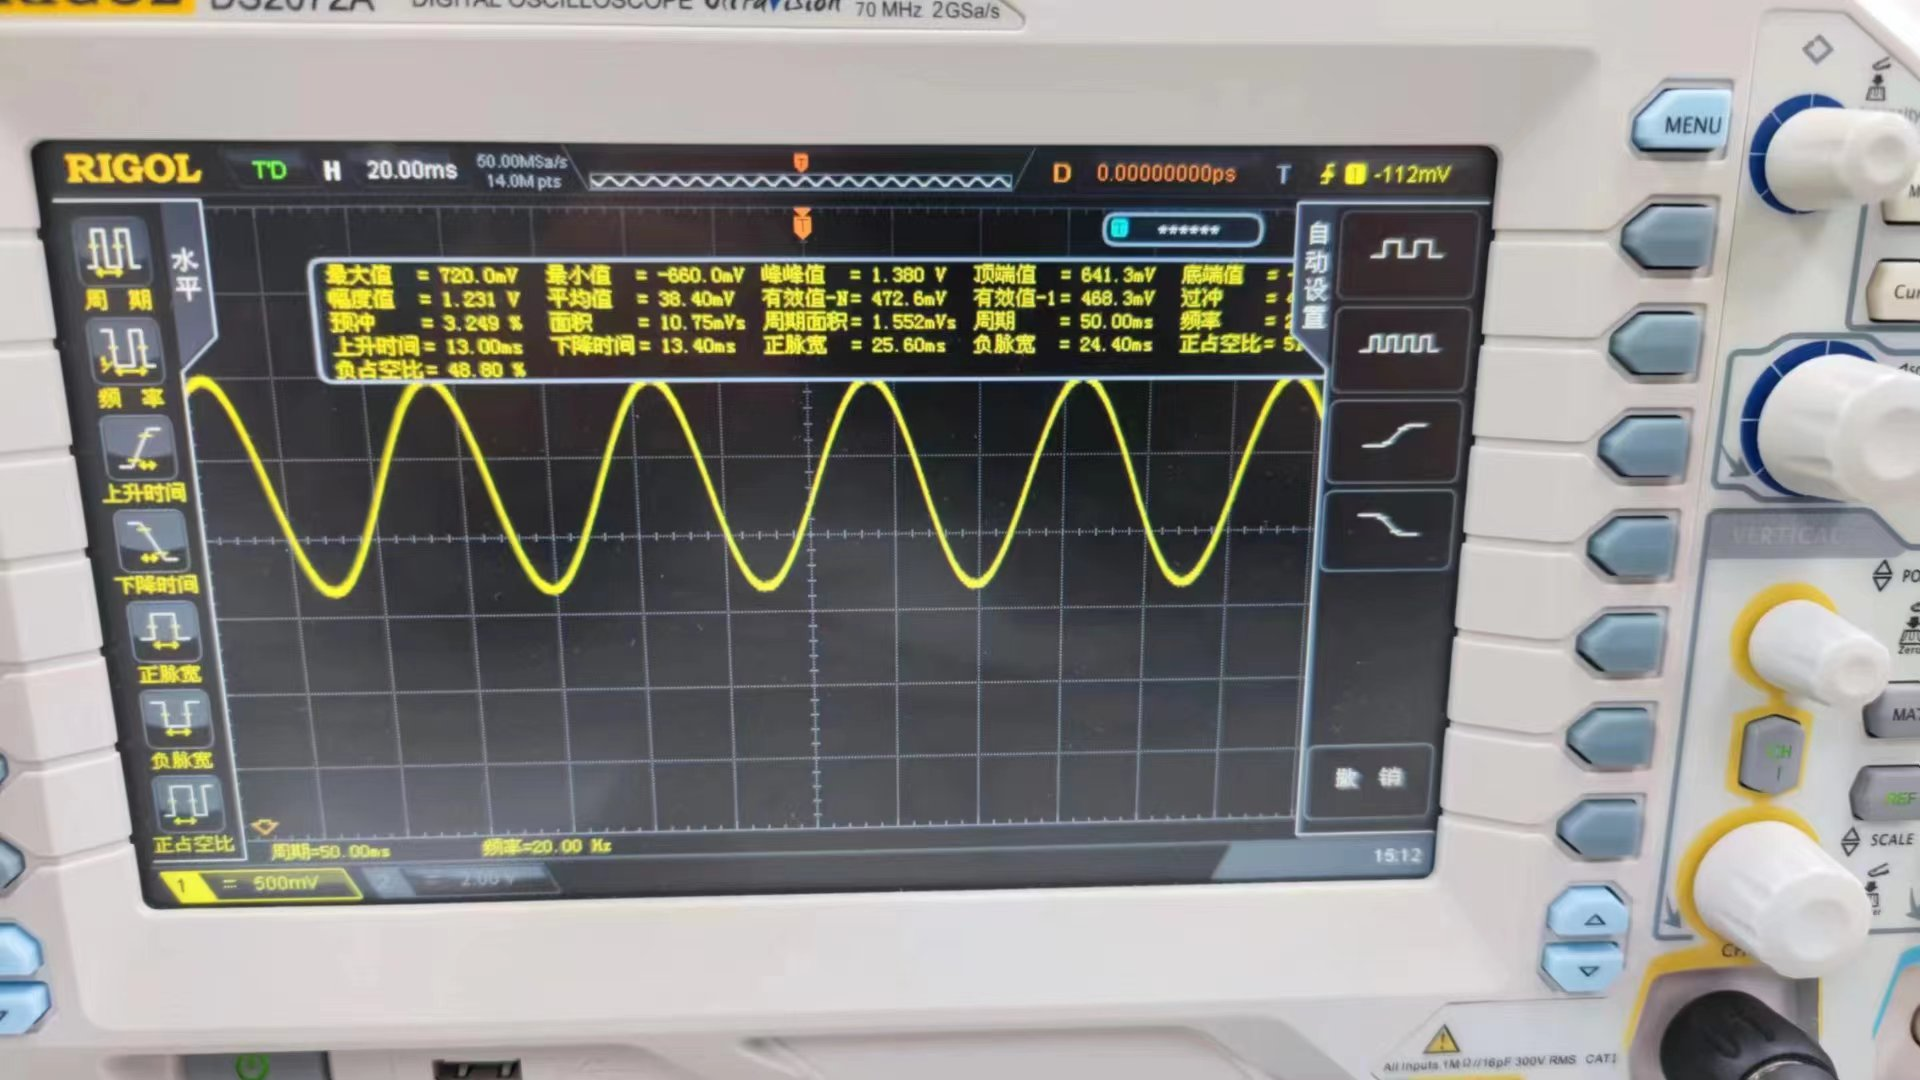
\includegraphics[width=0.9\linewidth]{低通滤波20Hz}%%%%%%%%%note3
			\caption{低通滤波20Hz}
			\label{低通滤波20Hz}
		\end{minipage}%
		\begin{minipage}[t]{0.49\linewidth}
			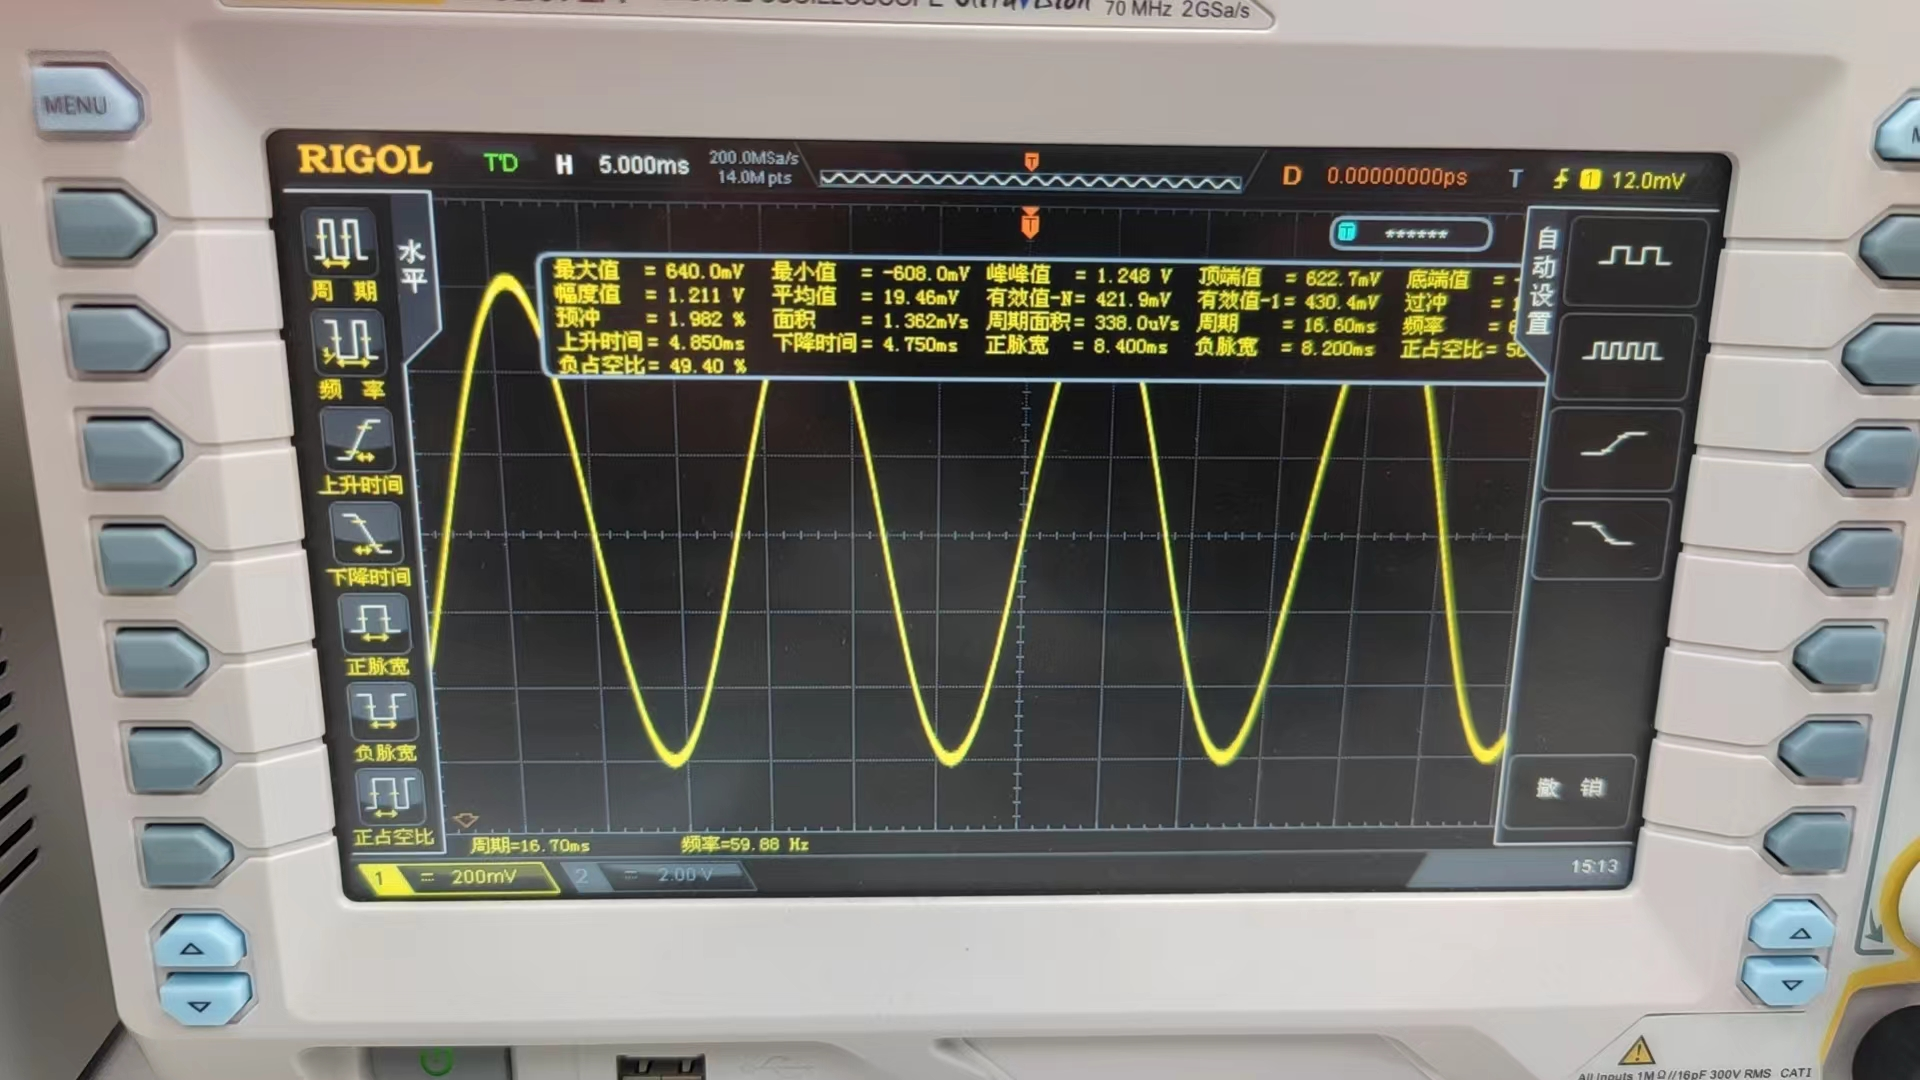
\includegraphics[width=0.9\linewidth]{低通滤波60Hz}
			\caption{低通滤波60Hz}
			\label{低通滤波60Hz}
		\end{minipage}
	
		\begin{minipage}[t]{0.49\linewidth}%%%%%%%%%note2
			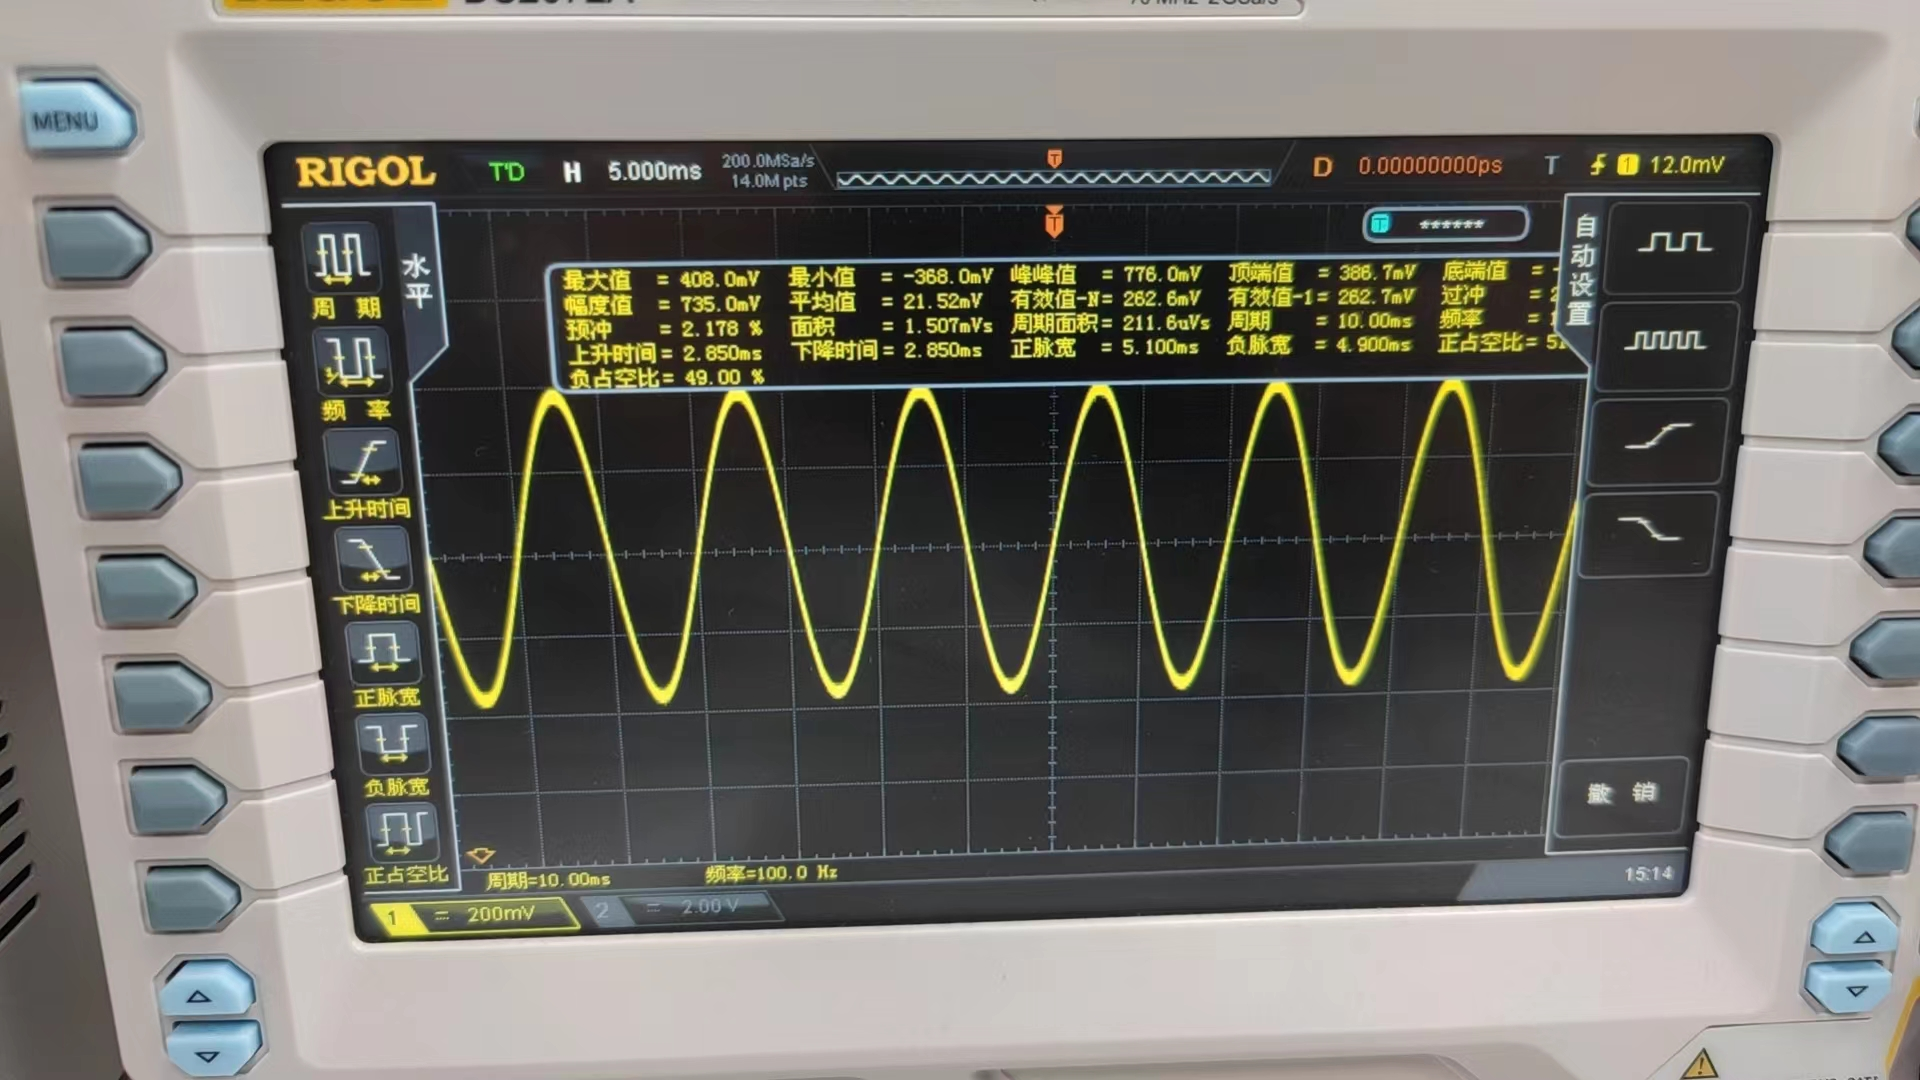
\includegraphics[width=0.9\linewidth]{低通滤波100Hz}%%%%%%%%%note3
			\caption{低通滤波100Hz}
			\label{低通滤波100Hz}
		\end{minipage}%
		\begin{minipage}[t]{0.49\linewidth}%%%%%%%%%note2
			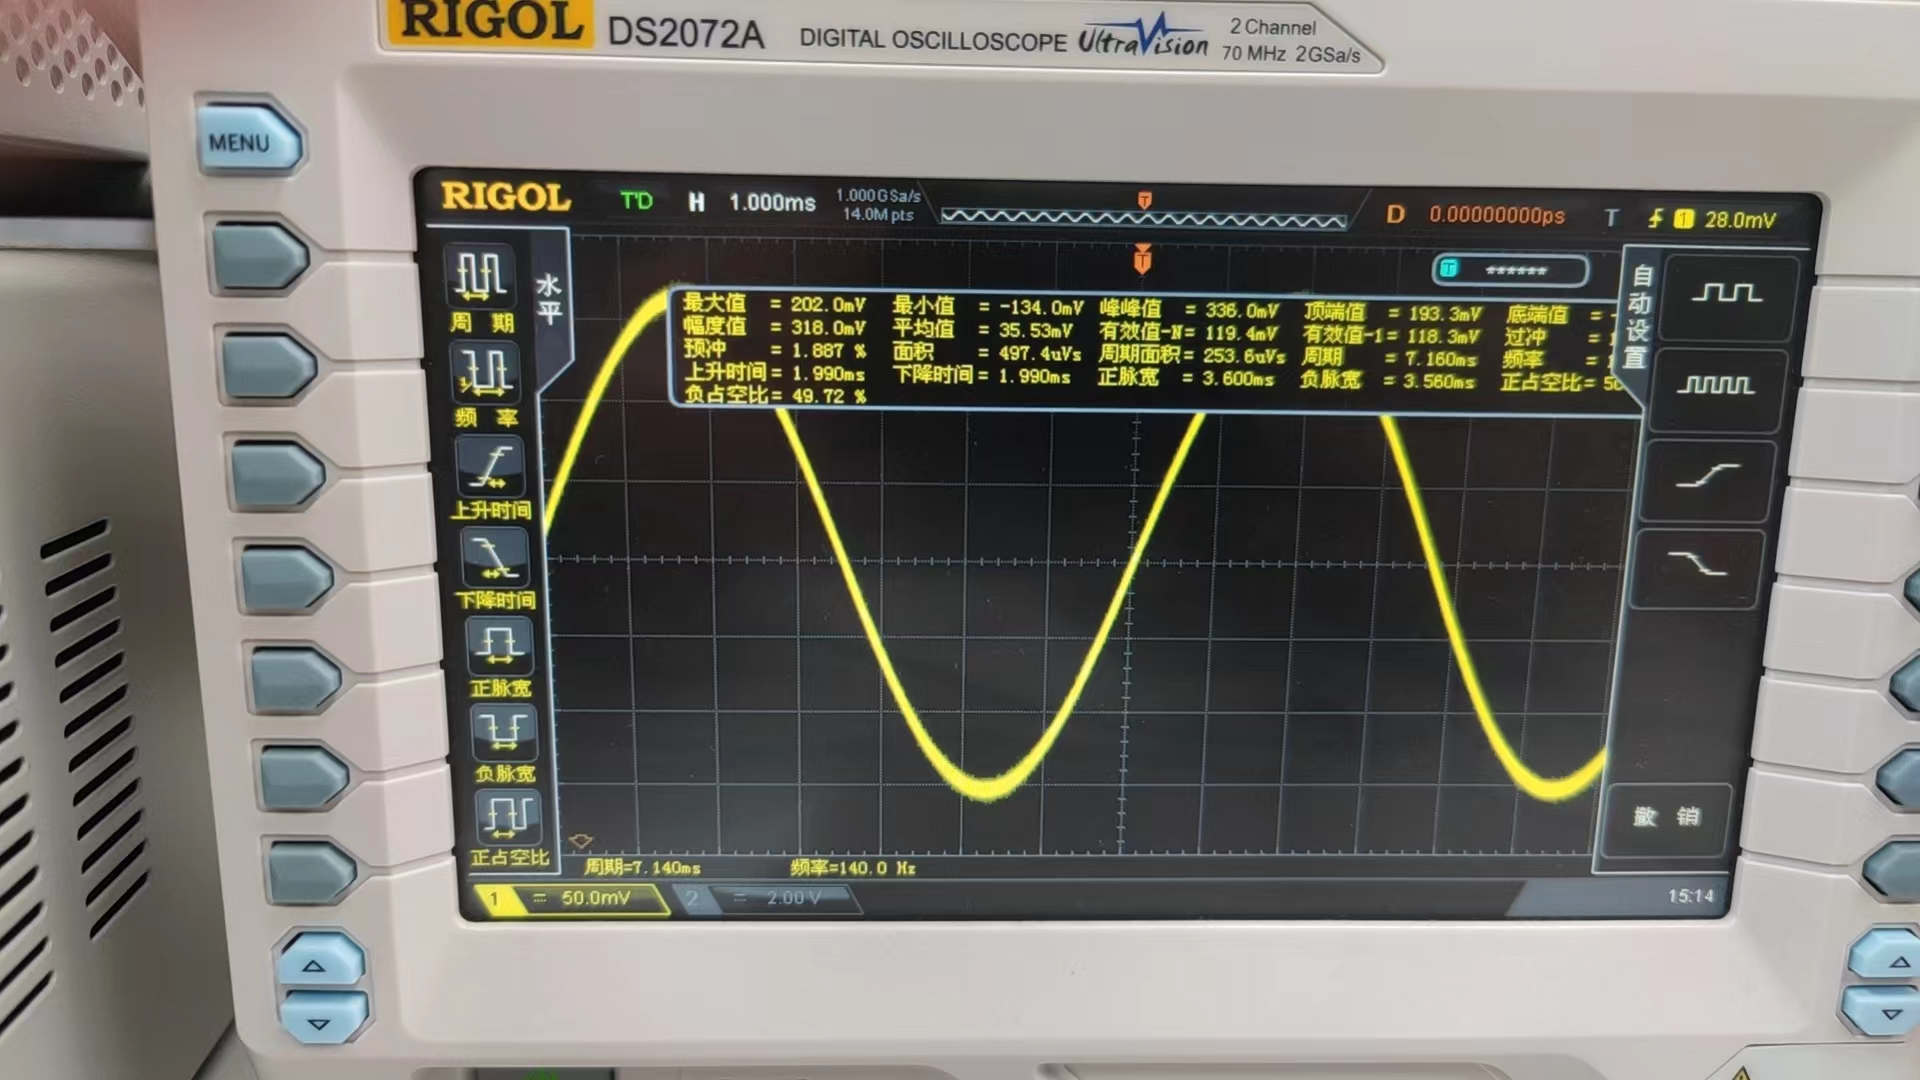
\includegraphics[width=0.9\linewidth]{低通滤波140Hz}%%%%%%%%%note3
			\caption{低通滤波140Hz}
			\label{低通滤波140Hz}
		\end{minipage}%
	\end{figure}

	\begin{table}[htbp]
		\centering
		\begin{tabular}{ c|c|c|c|c|c|c|c p{1.5cm}|}
			\hline
			频率(Hz) & 20 & 40 & 60 & 80 & 100 & 120 & 140 \\
			\hline
			峰峰值(V)  & 1.380 & 1.328 & 1.248 & 1.040 & 0.776 & 0.528 & 0.336 \\
			\hline
		\end{tabular}
		\caption{低通滤波20Hz到140Hz测量结果}\label{低通滤波20Hz到140Hz测量结果}
	\end{table}

	我们将表中的测试结果绘制成曲线图,能够更好地看出低通滤波的效果,曲线图如图\ref{低通滤波}所示。从曲线图中,我们可以看出该低通滤波器是可以正常工作、达到低通滤波的效果,并且当其峰峰值下降至-3dB时,频率为84Hz左右,所以该低通滤波器的效果还是不错的,带外的抑制效果也能达到要求。
	
	\begin{figure}[h]
		\centering%使该部分内容居中
		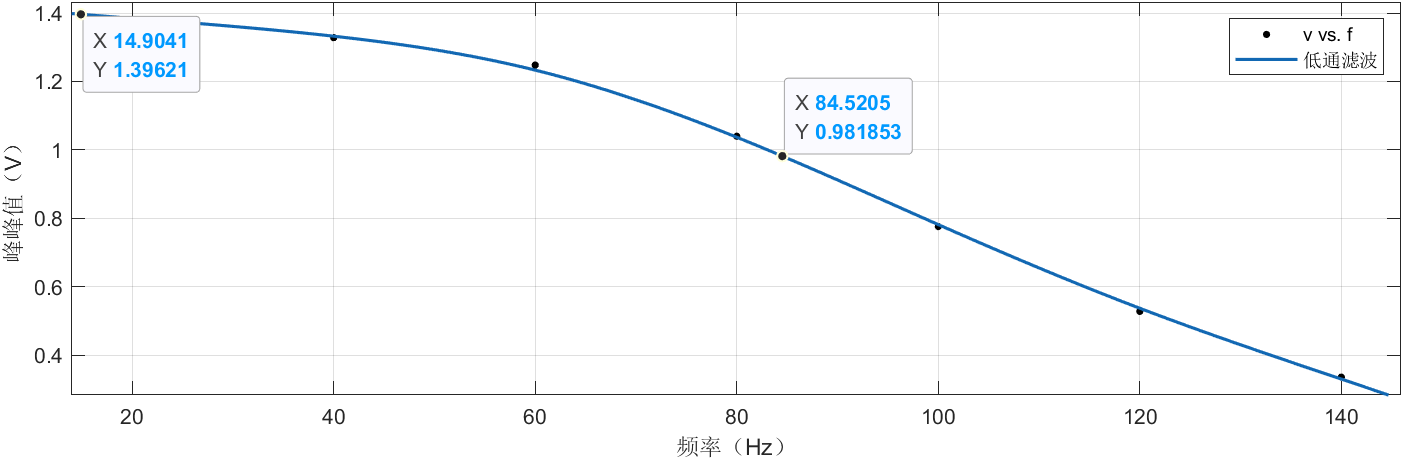
\includegraphics[width=6in]{低通滤波}
		\caption{低通滤波}%命名并编号
		\label{低通滤波}%设置标签
	\end{figure}

	
	\subsubsection{高通滤波部分}

	\begin{figure}[H]
		\centering
		\begin{minipage}[t]{0.4\linewidth}%%%%%%%%%note2
			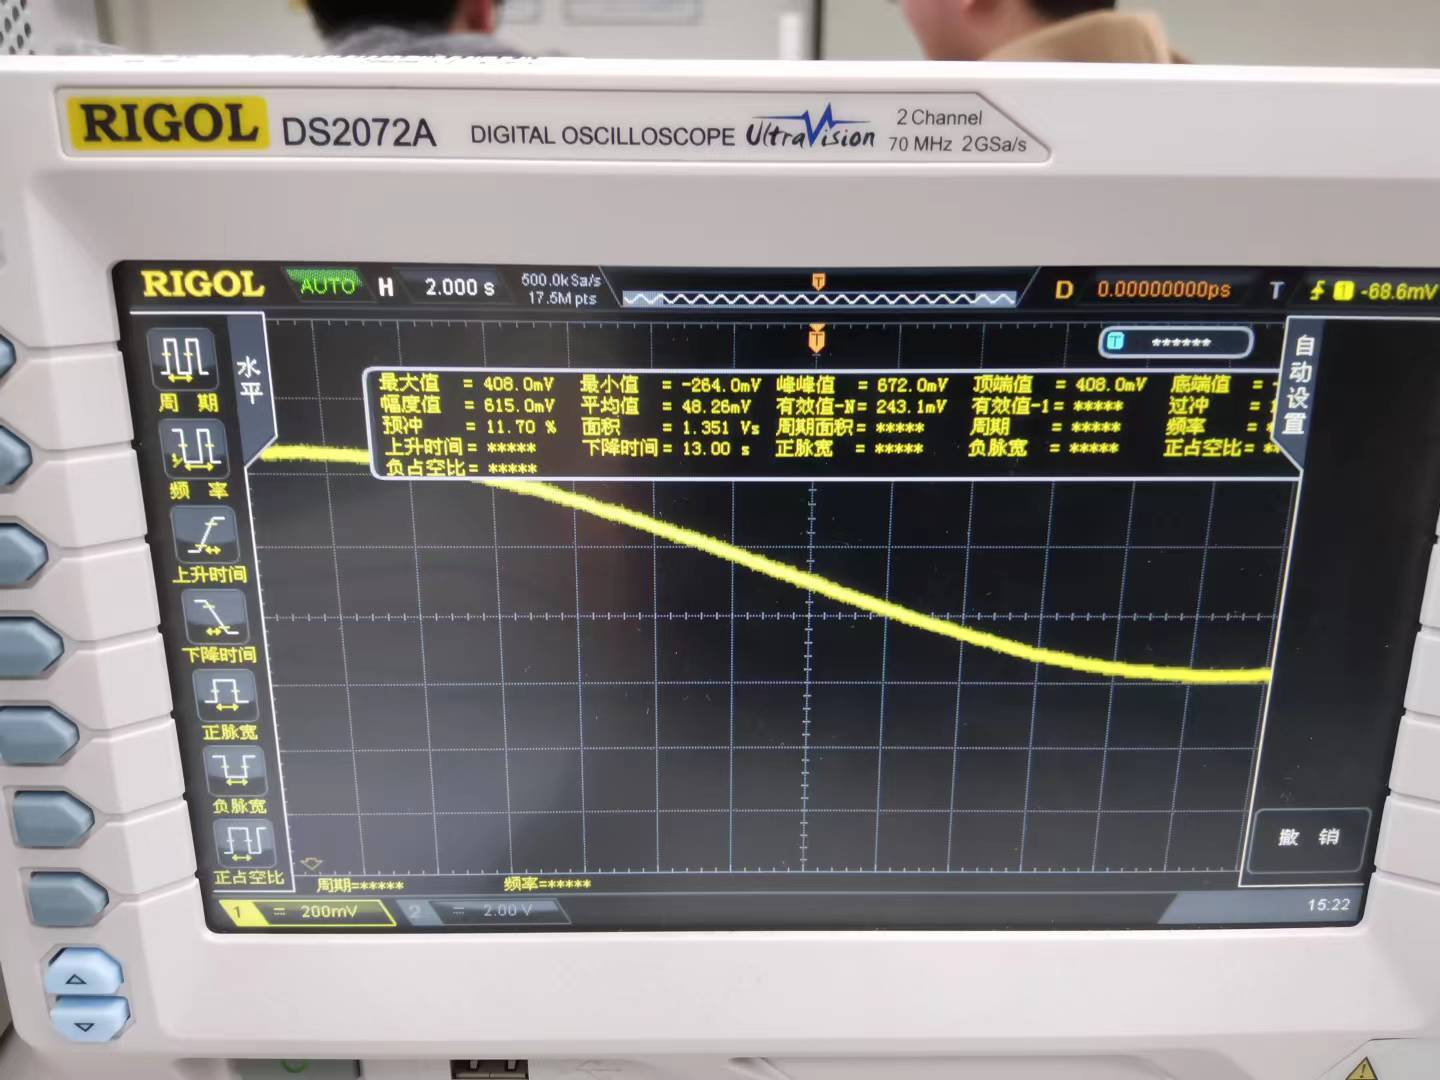
\includegraphics[width=0.9\linewidth]{高通滤波20mHz}%%%%%%%%%note3
			\caption{高通滤波20mHz}
			\label{高通滤波20mHz}
		\end{minipage}%
		\begin{minipage}[t]{0.4\linewidth}
			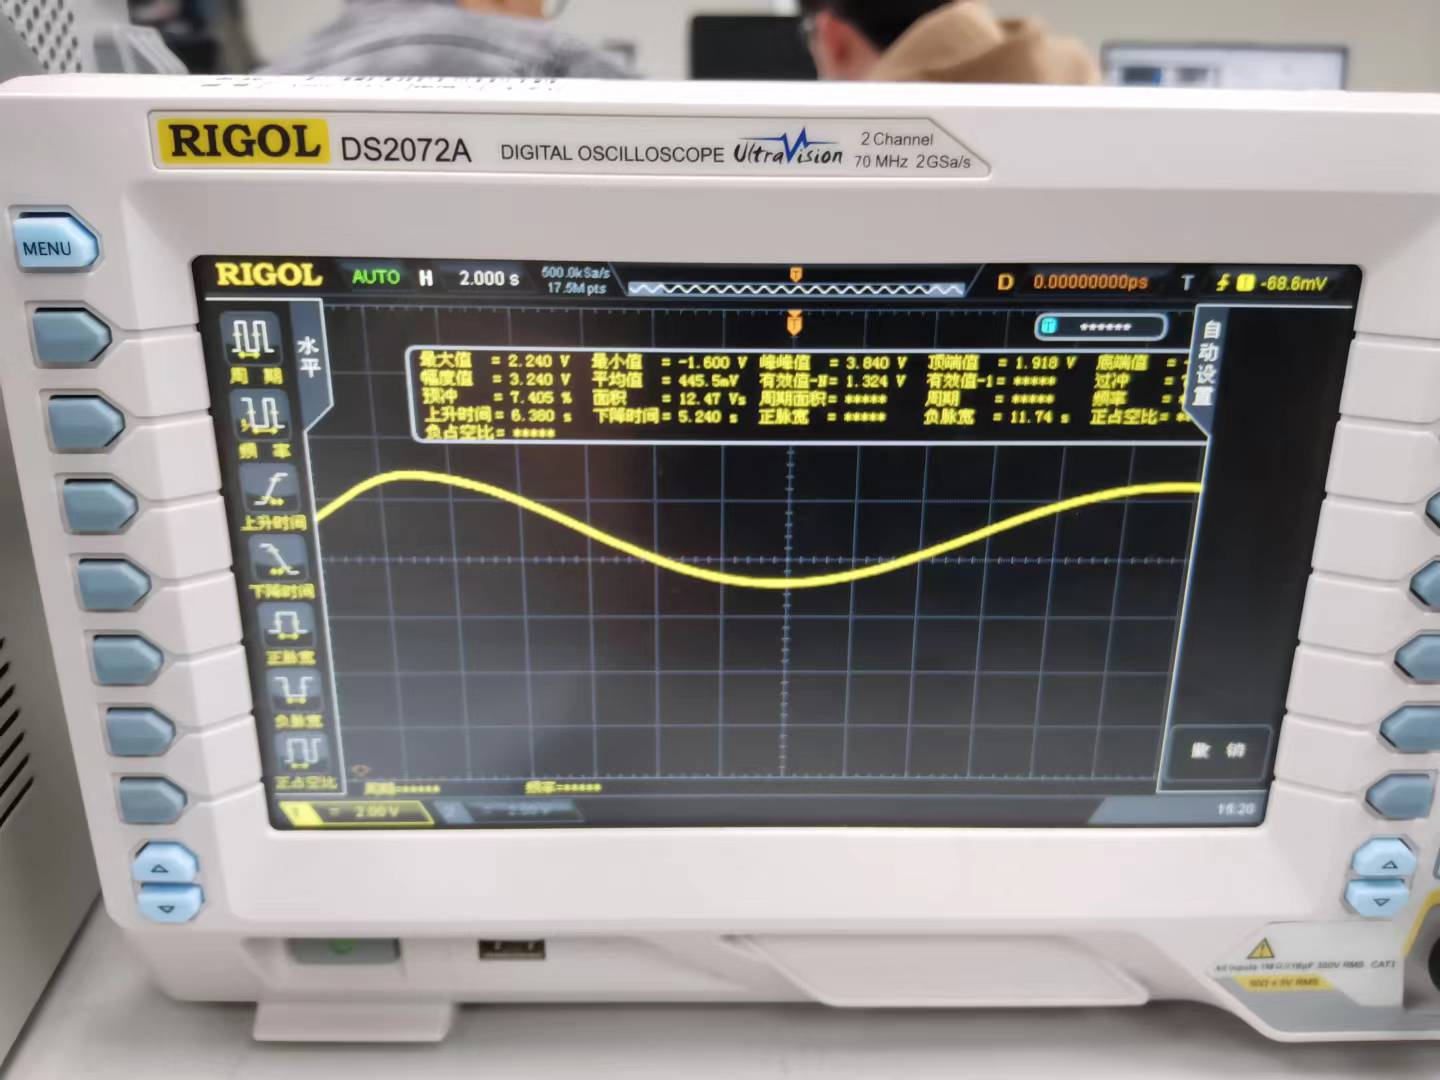
\includegraphics[width=0.9\linewidth]{高通滤波40mHz}
			\caption{高通滤波40mHz}
			\label{高通滤波40mHz}
		\end{minipage}
		
		\begin{minipage}[t]{0.4\linewidth}%%%%%%%%%note2
			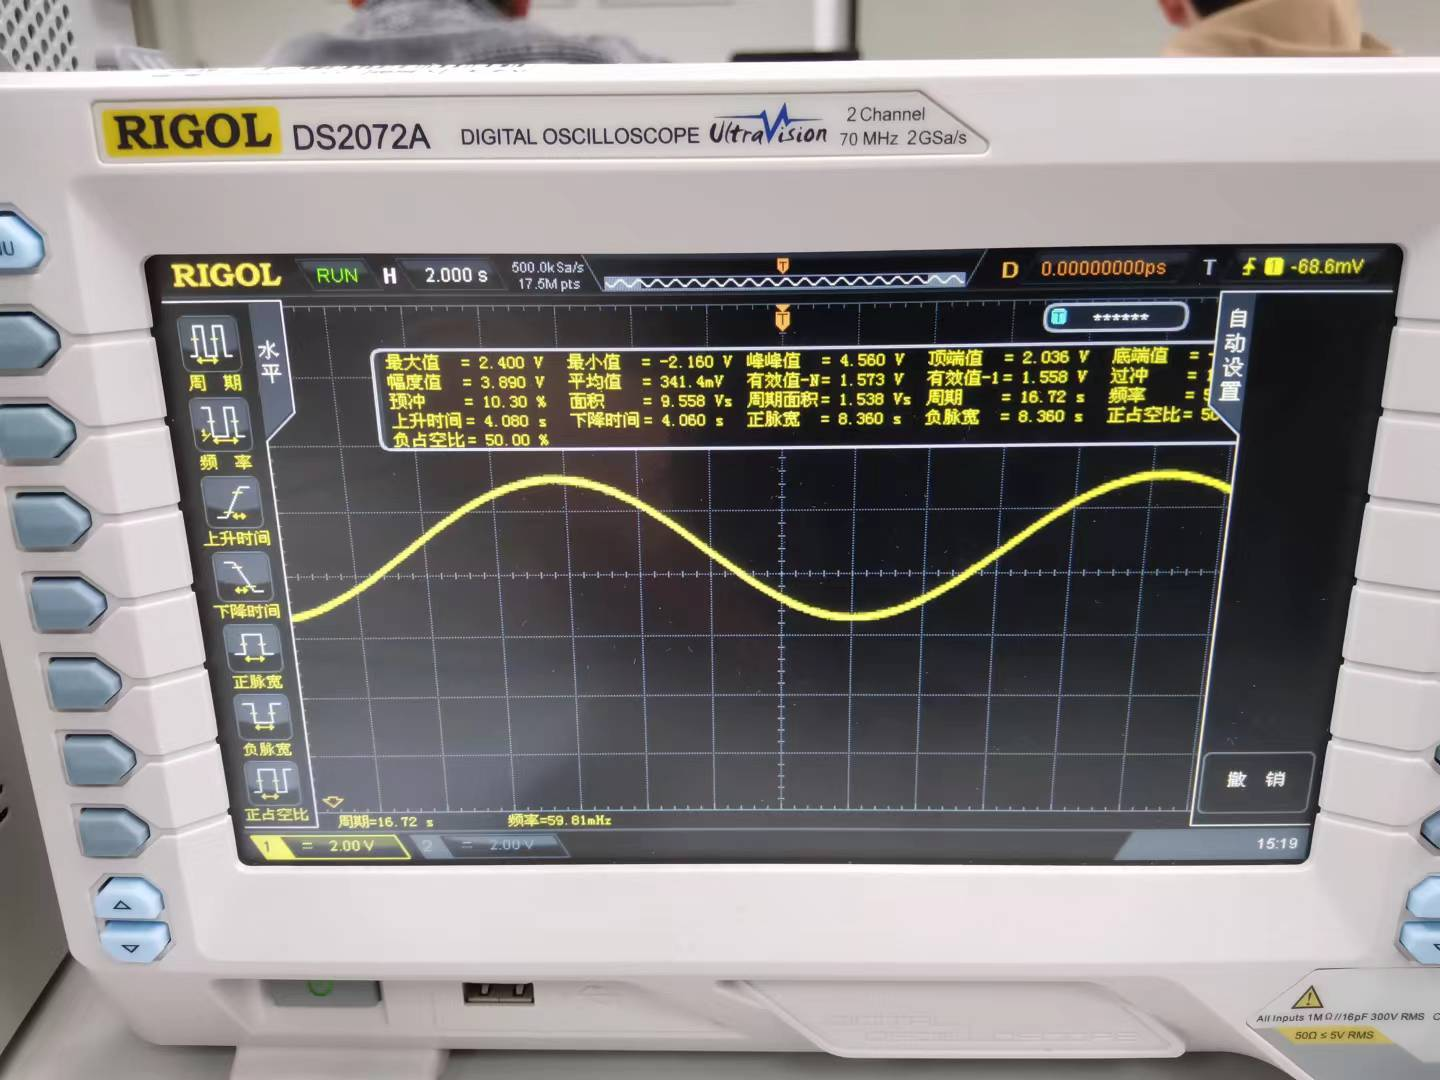
\includegraphics[width=0.9\linewidth]{高通滤波60mHz}%%%%%%%%%note3
			\caption{高通滤波60mHz}
			\label{高通滤波60mHz}
		\end{minipage}%
		\begin{minipage}[t]{0.4\linewidth}%%%%%%%%%note2
			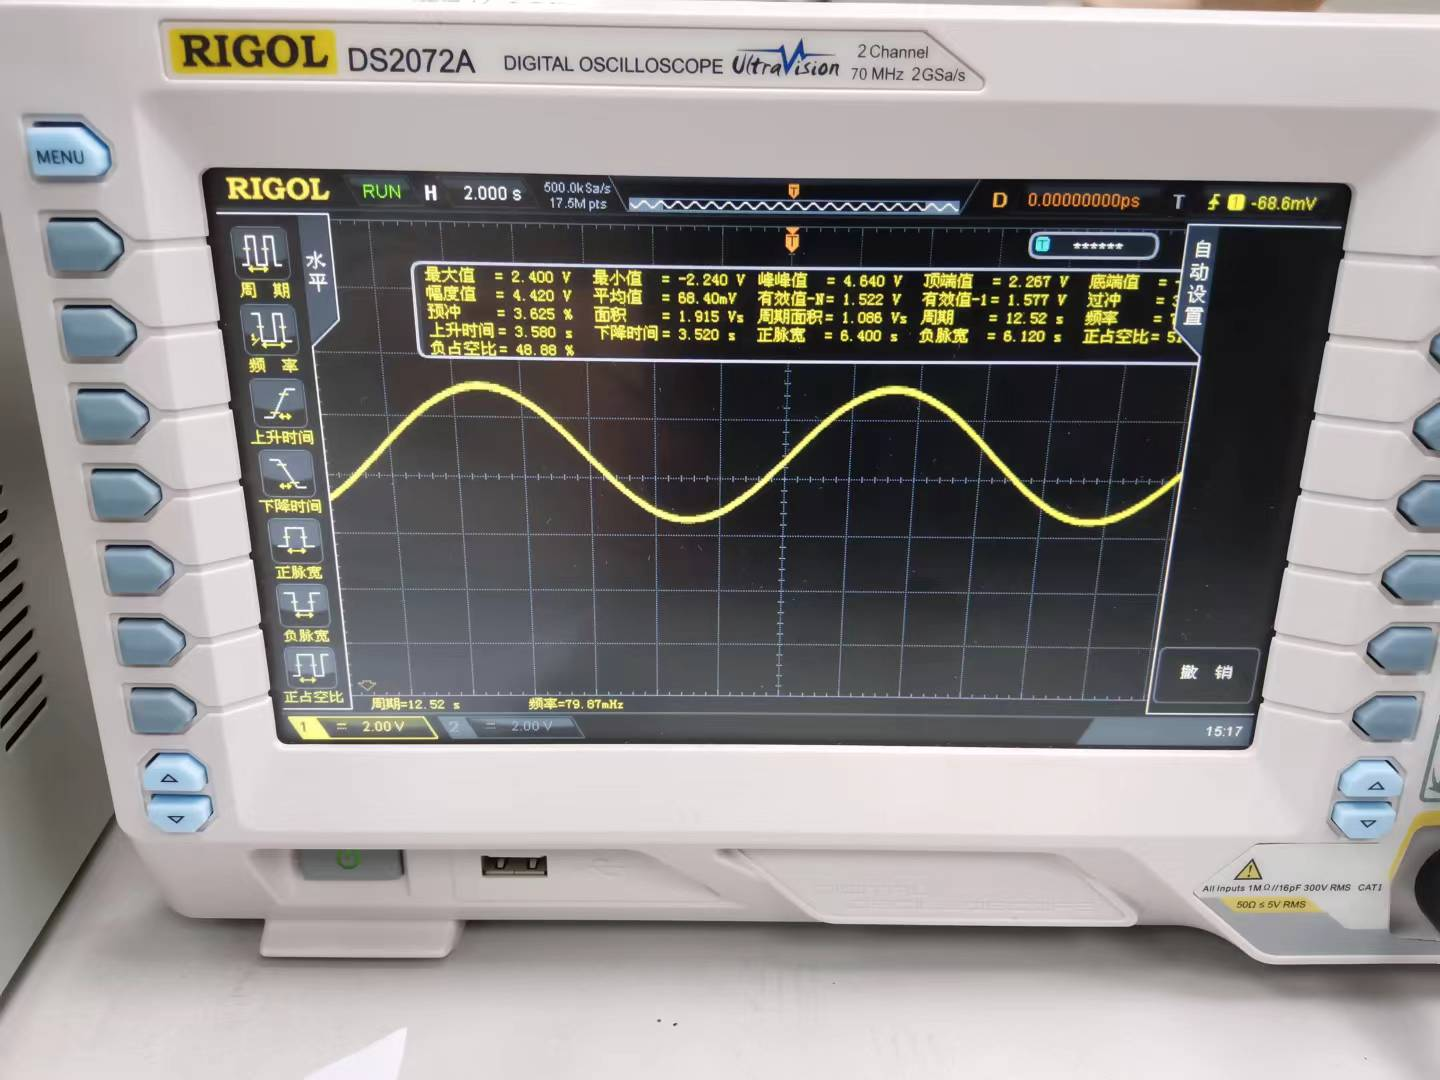
\includegraphics[width=0.9\linewidth]{高通滤波80mHz}%%%%%%%%%note3
			\caption{高通滤波80mHz}
			\label{高通滤波80mHz}
		\end{minipage}%
	\end{figure}

	在测试高通滤波部分时,主要针对20mHz到80mHz部分,测试图如图\ref{高通滤波20mHz}、\ref{高通滤波40mHz}、\ref{高通滤波60mHz}、\ref{高通滤波80mHz}所示,测试的数据如表\ref{高通滤波20mHz到100mHz测量结果}所示。将测试数据绘制成图像,能得到如图\ref{高通滤波}所示的曲线图。
	
	\begin{table}[htbp]
		\centering
		\begin{tabular}{ c|c|c|c|c p{1.5cm}}
			\hline
			频率(mHz) & 20 & 40 & 60 & 80  \\
			\hline
			峰峰值(V)  & 0.672 & 3.840 & 4.560 & 4.640 \\
			\hline
		\end{tabular}
		\caption{高通滤波20mHz到100mHz测量结果}\label{高通滤波20mHz到100mHz测量结果}
	\end{table}
	
	\begin{figure}[h]
		\centering%使该部分内容居中
		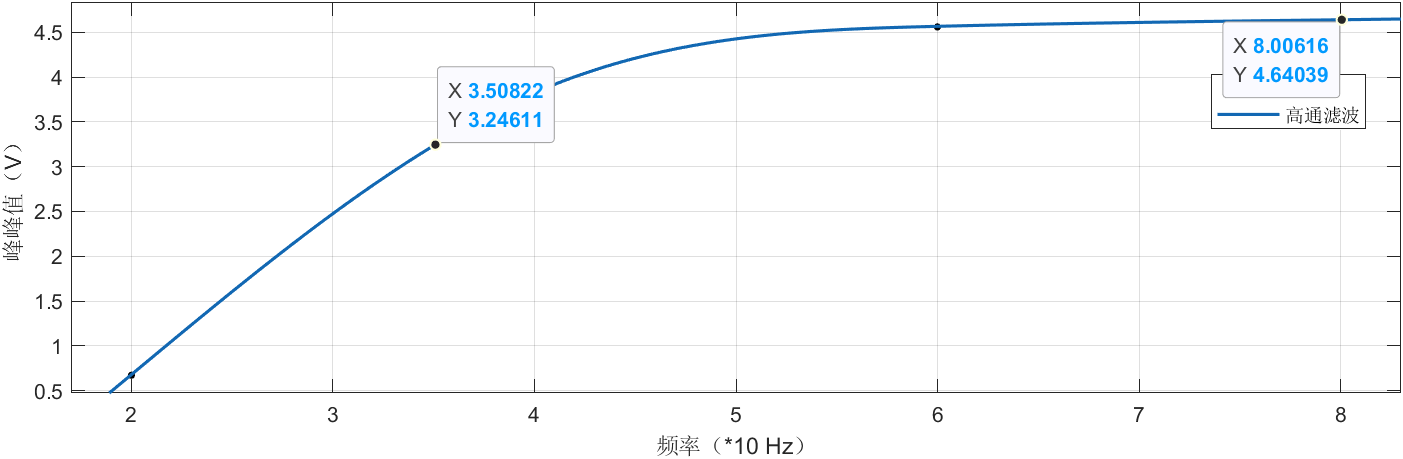
\includegraphics[width=6in]{高通滤波}
		\caption{高通滤波}%命名并编号
		\label{高通滤波}%设置标签
	\end{figure}

	从图中,我们能看出,高通滤波器能够正常工作并起到滤波的效果,当其峰峰值下降为-3dB时,频率约为35mHz,基本满足需求,同时带外抑制的效果也比较好。
	
	\subsubsection{陷波部分}
	
	在陷波部分,我们为得到陷波的频率,设置了从50Hz到35Hz的测试范围,如图\ref{陷波最低点}所示是测试时峰峰值最低点的图像。最终得到的测试数据如表\ref{陷波测试结果}所示。根据表中测试数据,我们绘制出陷波曲线,如图所示,能够更好地看出陷波地效果。
	
	\begin{figure}[H]
		\centering%使该部分内容居中
		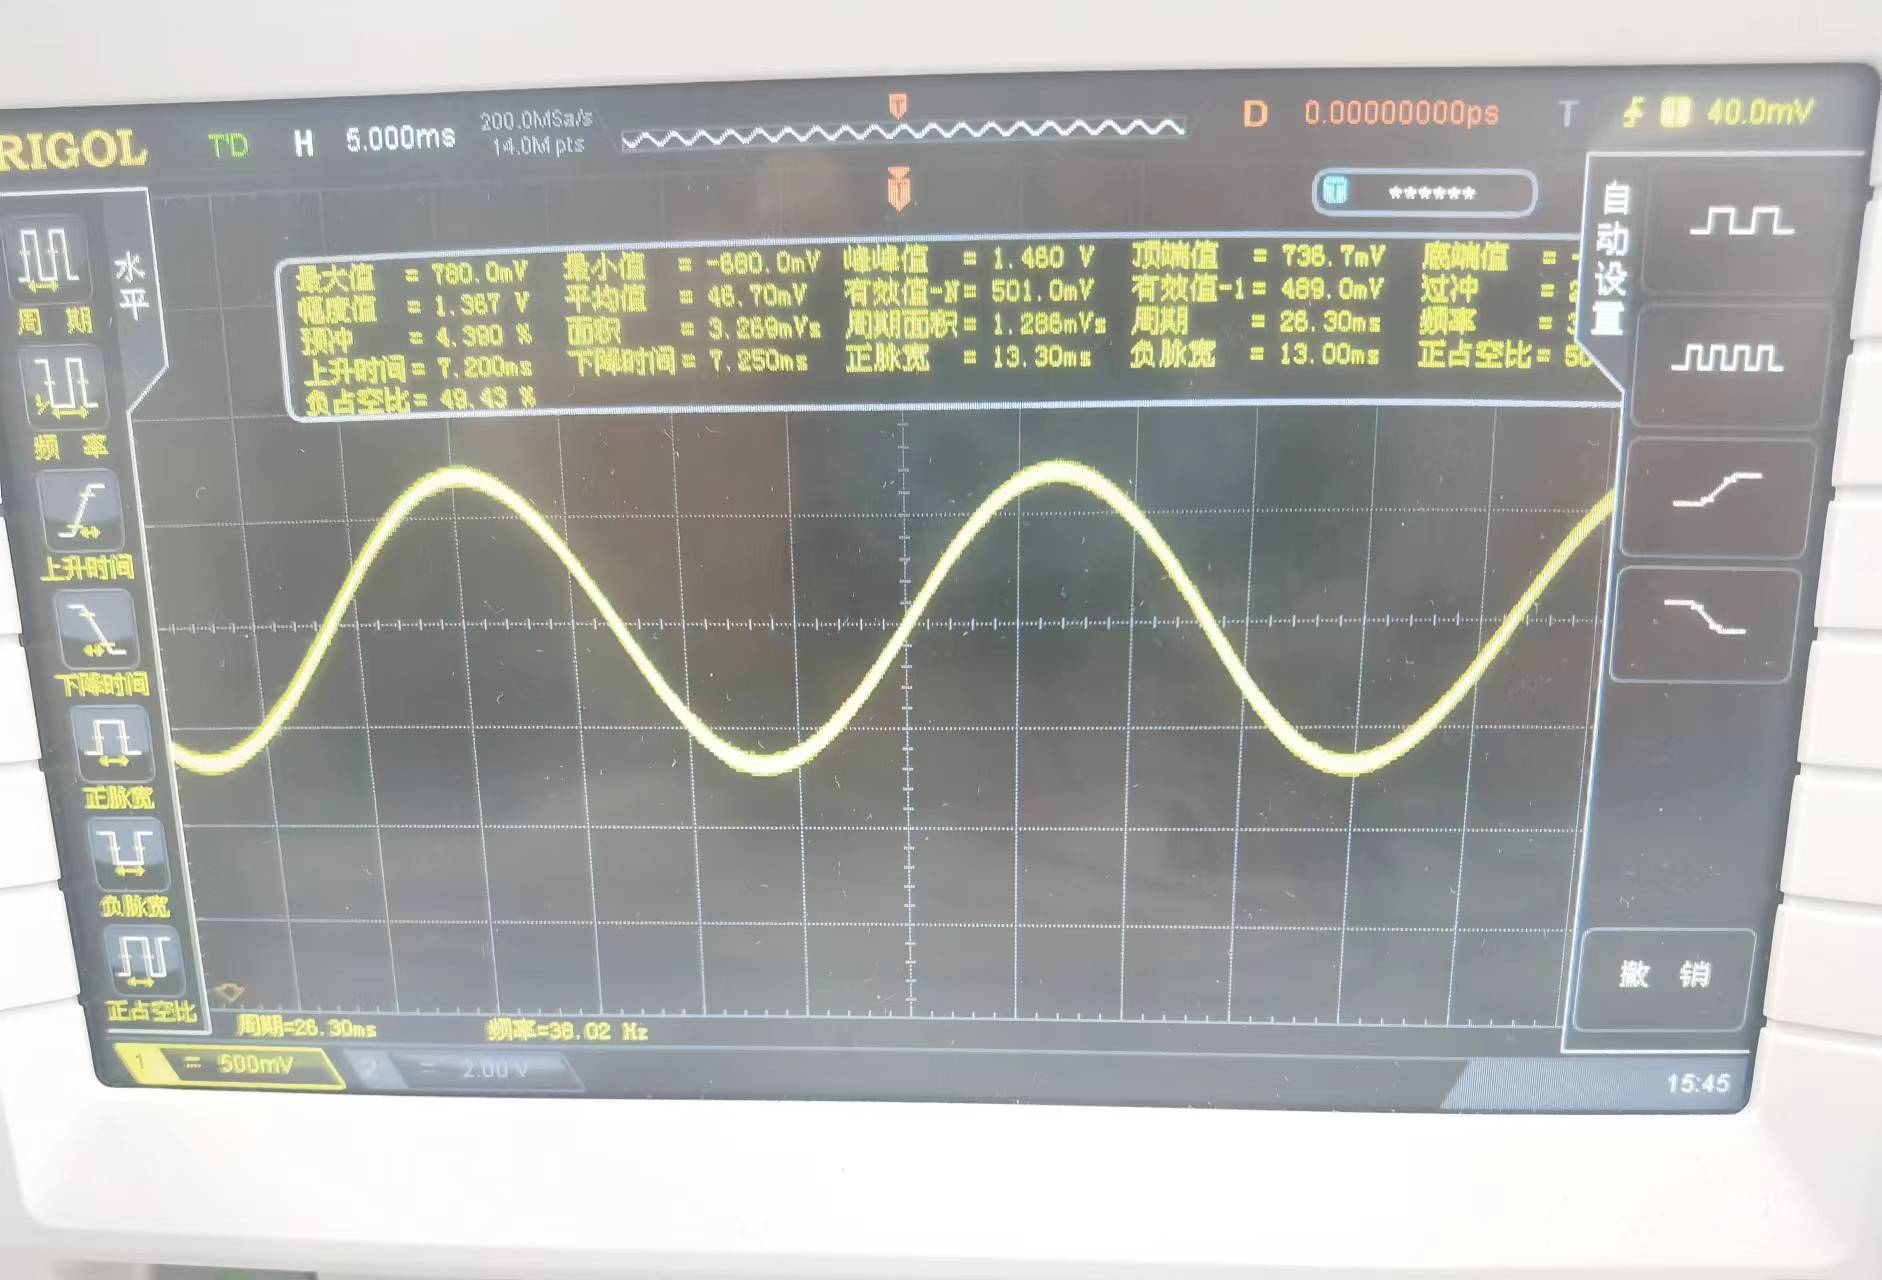
\includegraphics[width=3in]{陷波最低点}
		\caption{陷波最低点}%命名并编号
		\label{陷波最低点}%设置标签
	\end{figure}
	
	\begin{table}[htbp]
		\centering
		\begin{tabular}{ c|c|c|c|c|c|c|c|c p{1.5cm}}
			\hline
			频率(Hz) & 50 & 49 & 48 & 47 & 46 & 45 & 44 & 43  \\
			\hline
			峰峰值(V)  & 3.040 & 2.960 & 2.840 & 2.720 & 2.600 & 2.480 & 2.300 & 2.140 \\
			\hline
		\end{tabular}
	\end{table}

	\begin{table}[H]
		\centering
		\begin{tabular}{ c|c|c|c|c|c|c|c p{1.5cm}}
			\hline
			 42 & 41 & 40 & 39 & 38 & 37 & 36 & 35  \\
			\hline
			 1.980 & 1.800 & 1.640 & 1.560 & 1.460 & 1.520 & 1.640 & 1.880 \\
			\hline
		\end{tabular}
		\caption{陷波测试结果}\label{陷波测试结果}
	\end{table}

	\begin{figure}[H]
		\centering%使该部分内容居中
		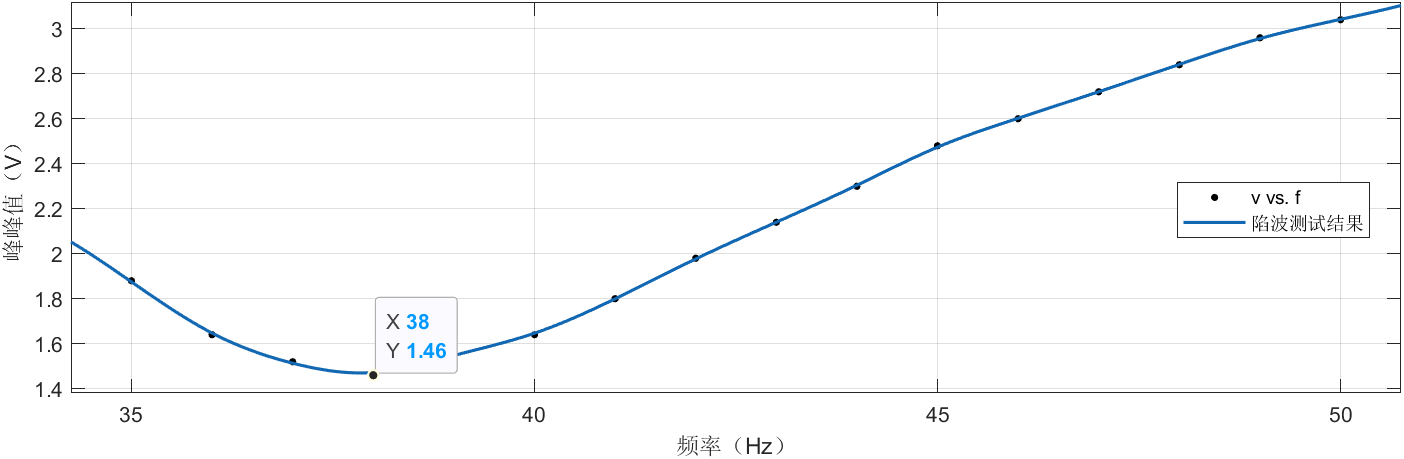
\includegraphics[width=6.5in]{陷波测试结果}
		\caption{陷波测试结果}%命名并编号
		\label{陷波测试结果图}%设置标签
	\end{figure}

	从图中,我们可以看出,陷波的中心位置为38Hz,更细致应该是在37到38Hz之间,而我们希望的陷波位置应该为40到50Hz之间,且该滤波测试结果中,陷波地带宽比较大,合格的陷波器的陷波位置应该是比较窄的,因此,陷波部分地效果并不理想。效果不理想的原因,最主要的应该是焊接使用的电容的电容值偏离指定值,导致陷波位置发生了偏移。
	
	\subsubsection{总体放大性能}
	
	在心电信号处理电路各个单独部分测试完成后,我们进行电路总体放大性能的测试,设置了20Hz到140Hz的测试范围,其测试结果如表\ref{总体性能测试结果}所示。根据表中数据,绘制得到如图\ref{总体放大性能}所示的曲线。
	
	\begin{table}[htbp]
		\centering
		\begin{tabular}{ c|c|c|c|c|c|c|c|c|c|c|c|c|c p{1.5cm}}
			\hline
			频率(Hz) & 20 & 30 & 40 &50 & 60 &70 & 80 &90 & 100 & 110 & 120 &130 & 140 \\
			\hline
			峰峰值(V)  & 2.580 & 2.120 & 0.900 & 1.780 & 2.160 & 2.200 & 2.060 & 1.840 & 1.580 & 1.380 & 1.140 & 0.960 & 0.752 \\
			\hline
		\end{tabular}
		\caption{总体性能测试结果}\label{总体性能测试结果}
	\end{table}

	\begin{figure}[H]
		\centering%使该部分内容居中
		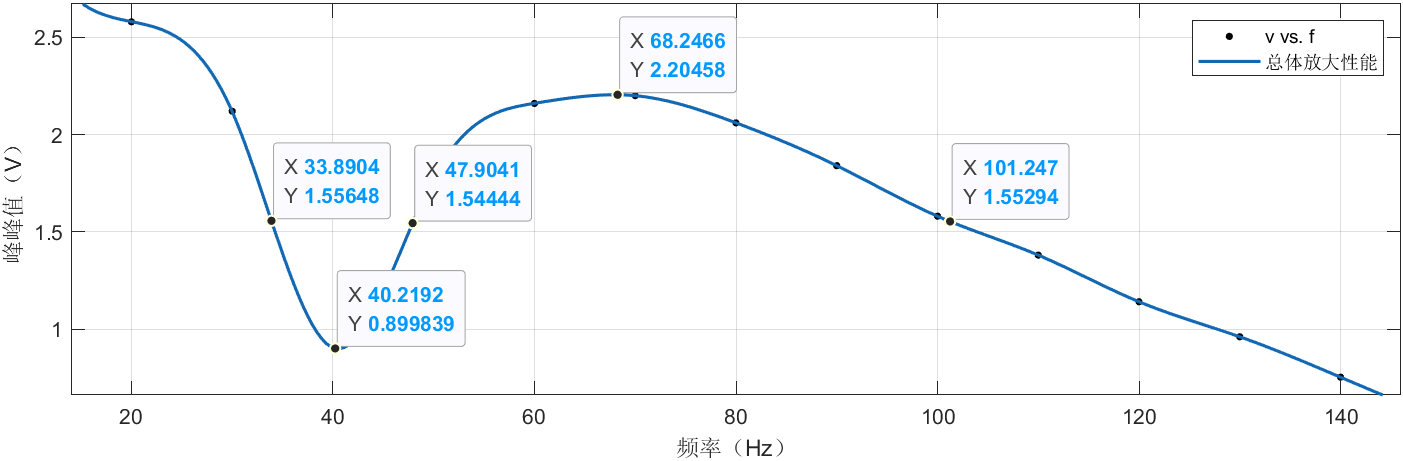
\includegraphics[width=6.5in]{总体放大性能}
		\caption{总体放大性能}%命名并编号
		\label{总体放大性能}%设置标签
	\end{figure}

	从图中可以看出,在40Hz左右发生陷波,在30Hz之前和45到101Hz之间增益较高,其余位置的抑制都较为明显,基本符合我们设计的初衷,能够起到总体处理和放大心电信号的作用。
	
	\subsubsection{人体测试}
	
	在测试完ECG信号检测调理电路的各类参数性能之后,我们进行人体测试,观察该电路实际能否起到处理心电信号,最终输出合格波形的作用。测试结果如图\ref{ECG信号检测调理电路_人体测试}所示。
	
	\begin{figure}[H]
		\centering%使该部分内容居中
		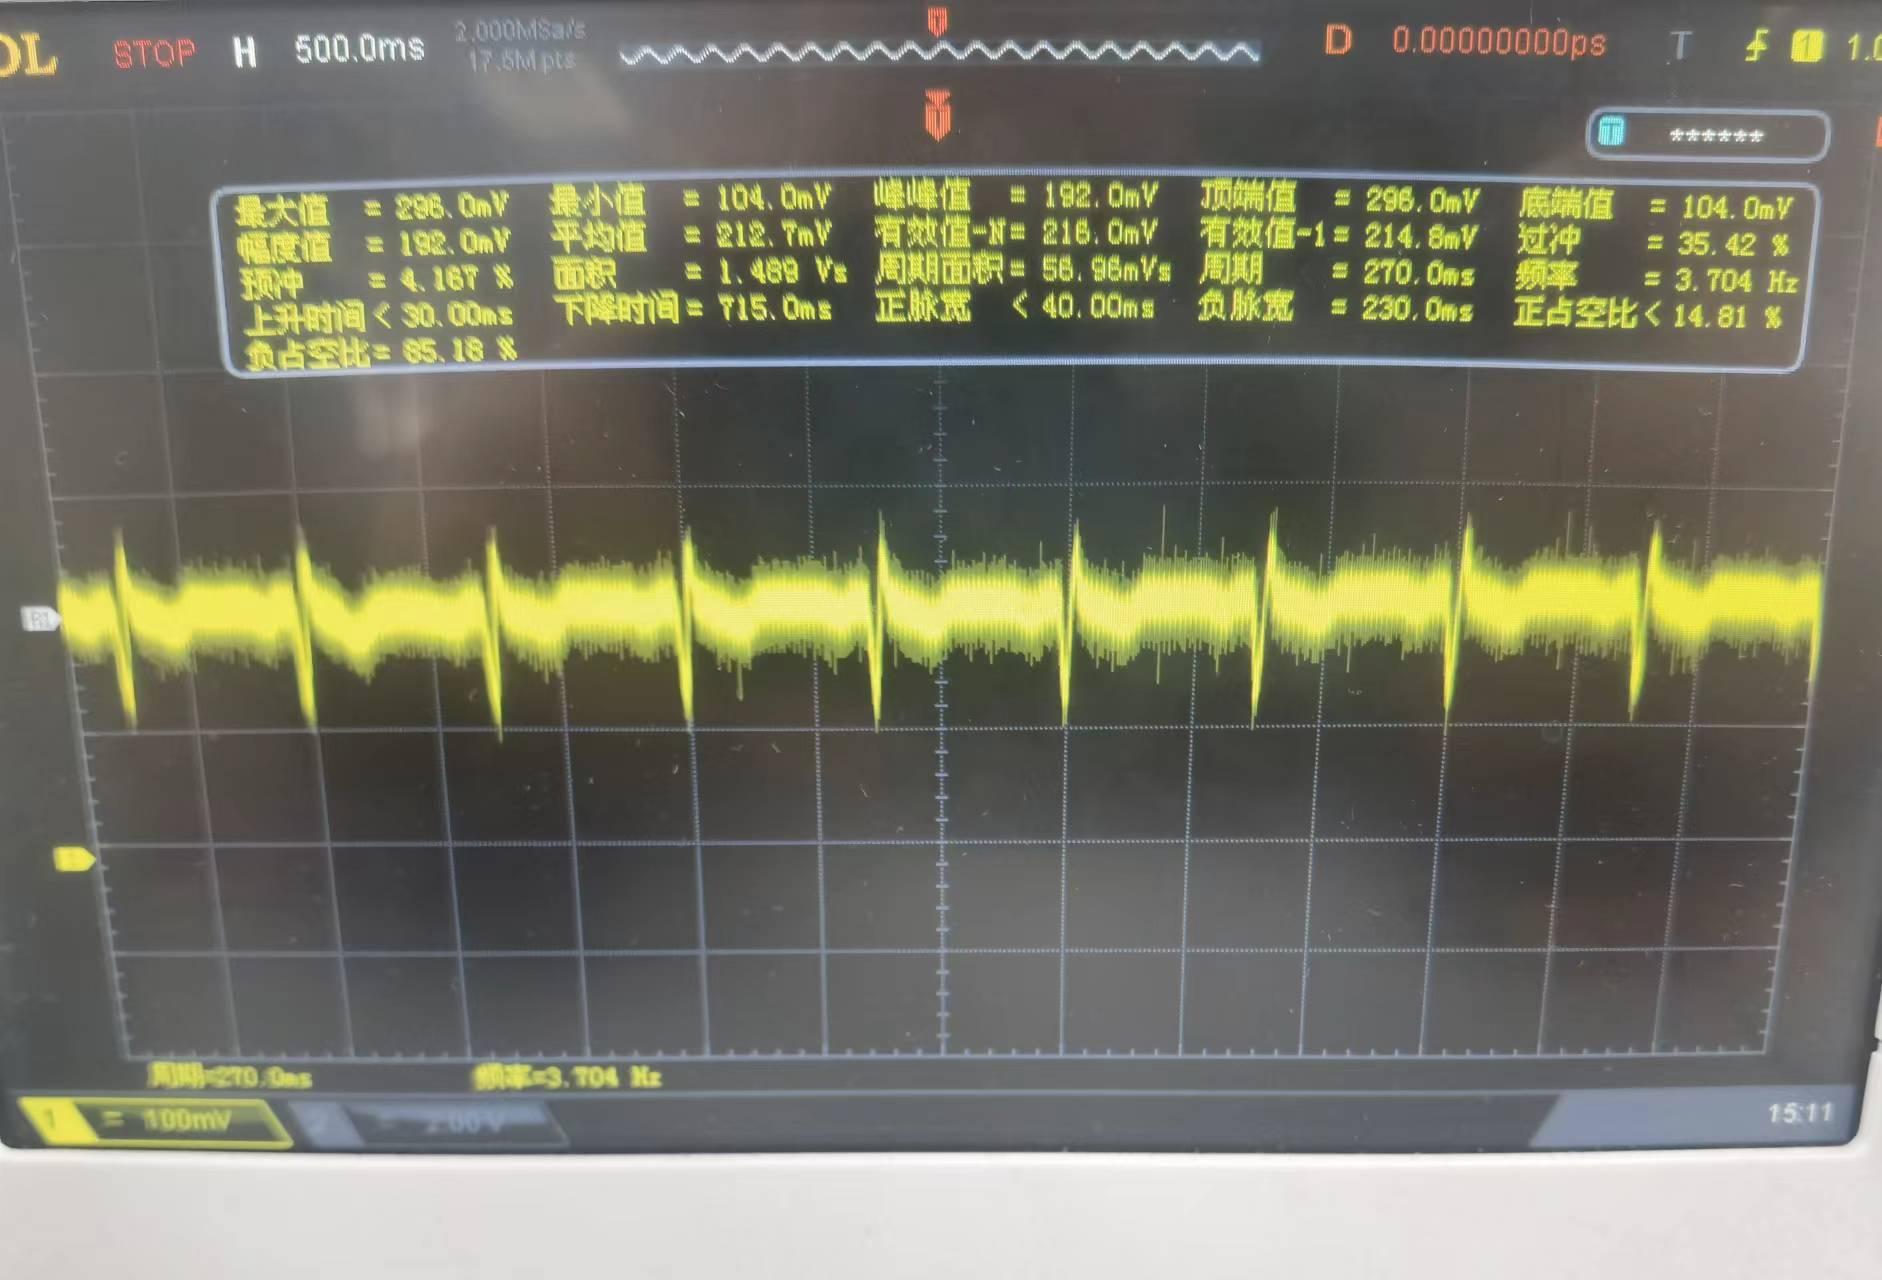
\includegraphics[width=4in]{ECG信号检测调理电路_人体测试}
		\caption{ECG信号检测调理电路-人体测试}%命名并编号
		\label{ECG信号检测调理电路_人体测试}%设置标签
	\end{figure}

	在示波器上,我们已经可以看出心电信号的波形,但同时,也发现其中混叠的杂波较多,心跳与心跳之间干扰明显,心电信号的增益还不够大,容易和杂波混在一起。
	
	\newpage
	
	\section{ECG心电监测系统}
	
	\subsection{总体目标}
	
	\subsubsection{系统框图及功能说明}
	
	ECG心电检测系统是由ECG信号检测调理电路同通信模块集成而成,主要用于实时检测人体心电信号,并发送到监测端,从而达到远程的心电监测。该ECG心电监测系统的系统框图及功能说明如图\ref{ECG系统框图}所示。
	
	\begin{figure}[H]
		\centering%使该部分内容居中
		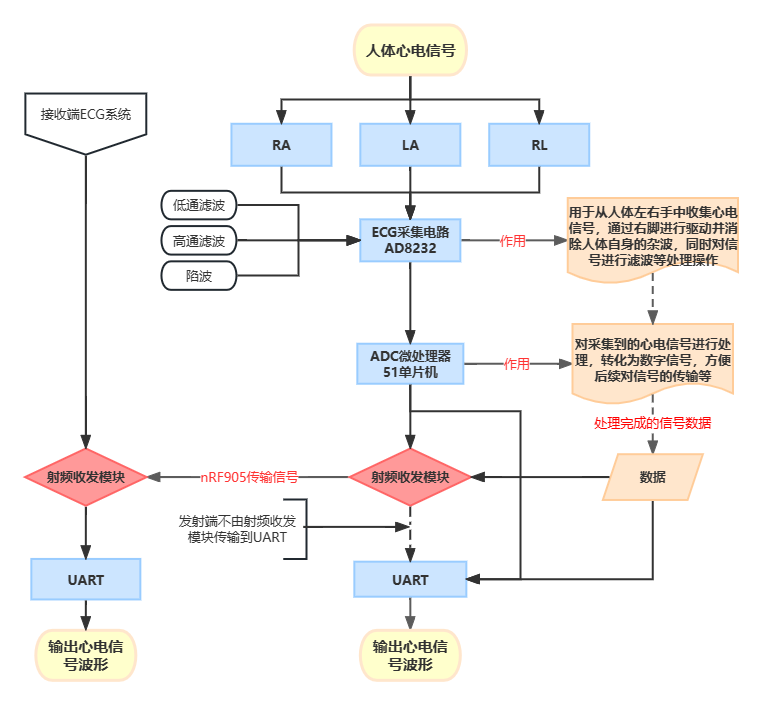
\includegraphics[width=6.5in]{ECG系统框图}
		\caption{ECG系统框图}%命名并编号
		\label{ECG系统框图}%设置标签
	\end{figure}
	
	\newpage
	
	\subsection{硬件设计}
	
	\subsubsection{原理图设计}
	
	根据ECG心电监测系统的系统框图,我们也可以将系统设计大体分为三个部分,其具体设计及电路连接如图\ref{ECG电路原理图_前端信号接收处理部分}、\ref{ECG电路原理图_中间ADC处理部分}、\ref{ECG电路原理图_后端通信与输出部分}所示。
	
	\begin{figure}[H]
		\centering
		\begin{minipage}[t]{0.49\linewidth}%%%%%%%%%note2
			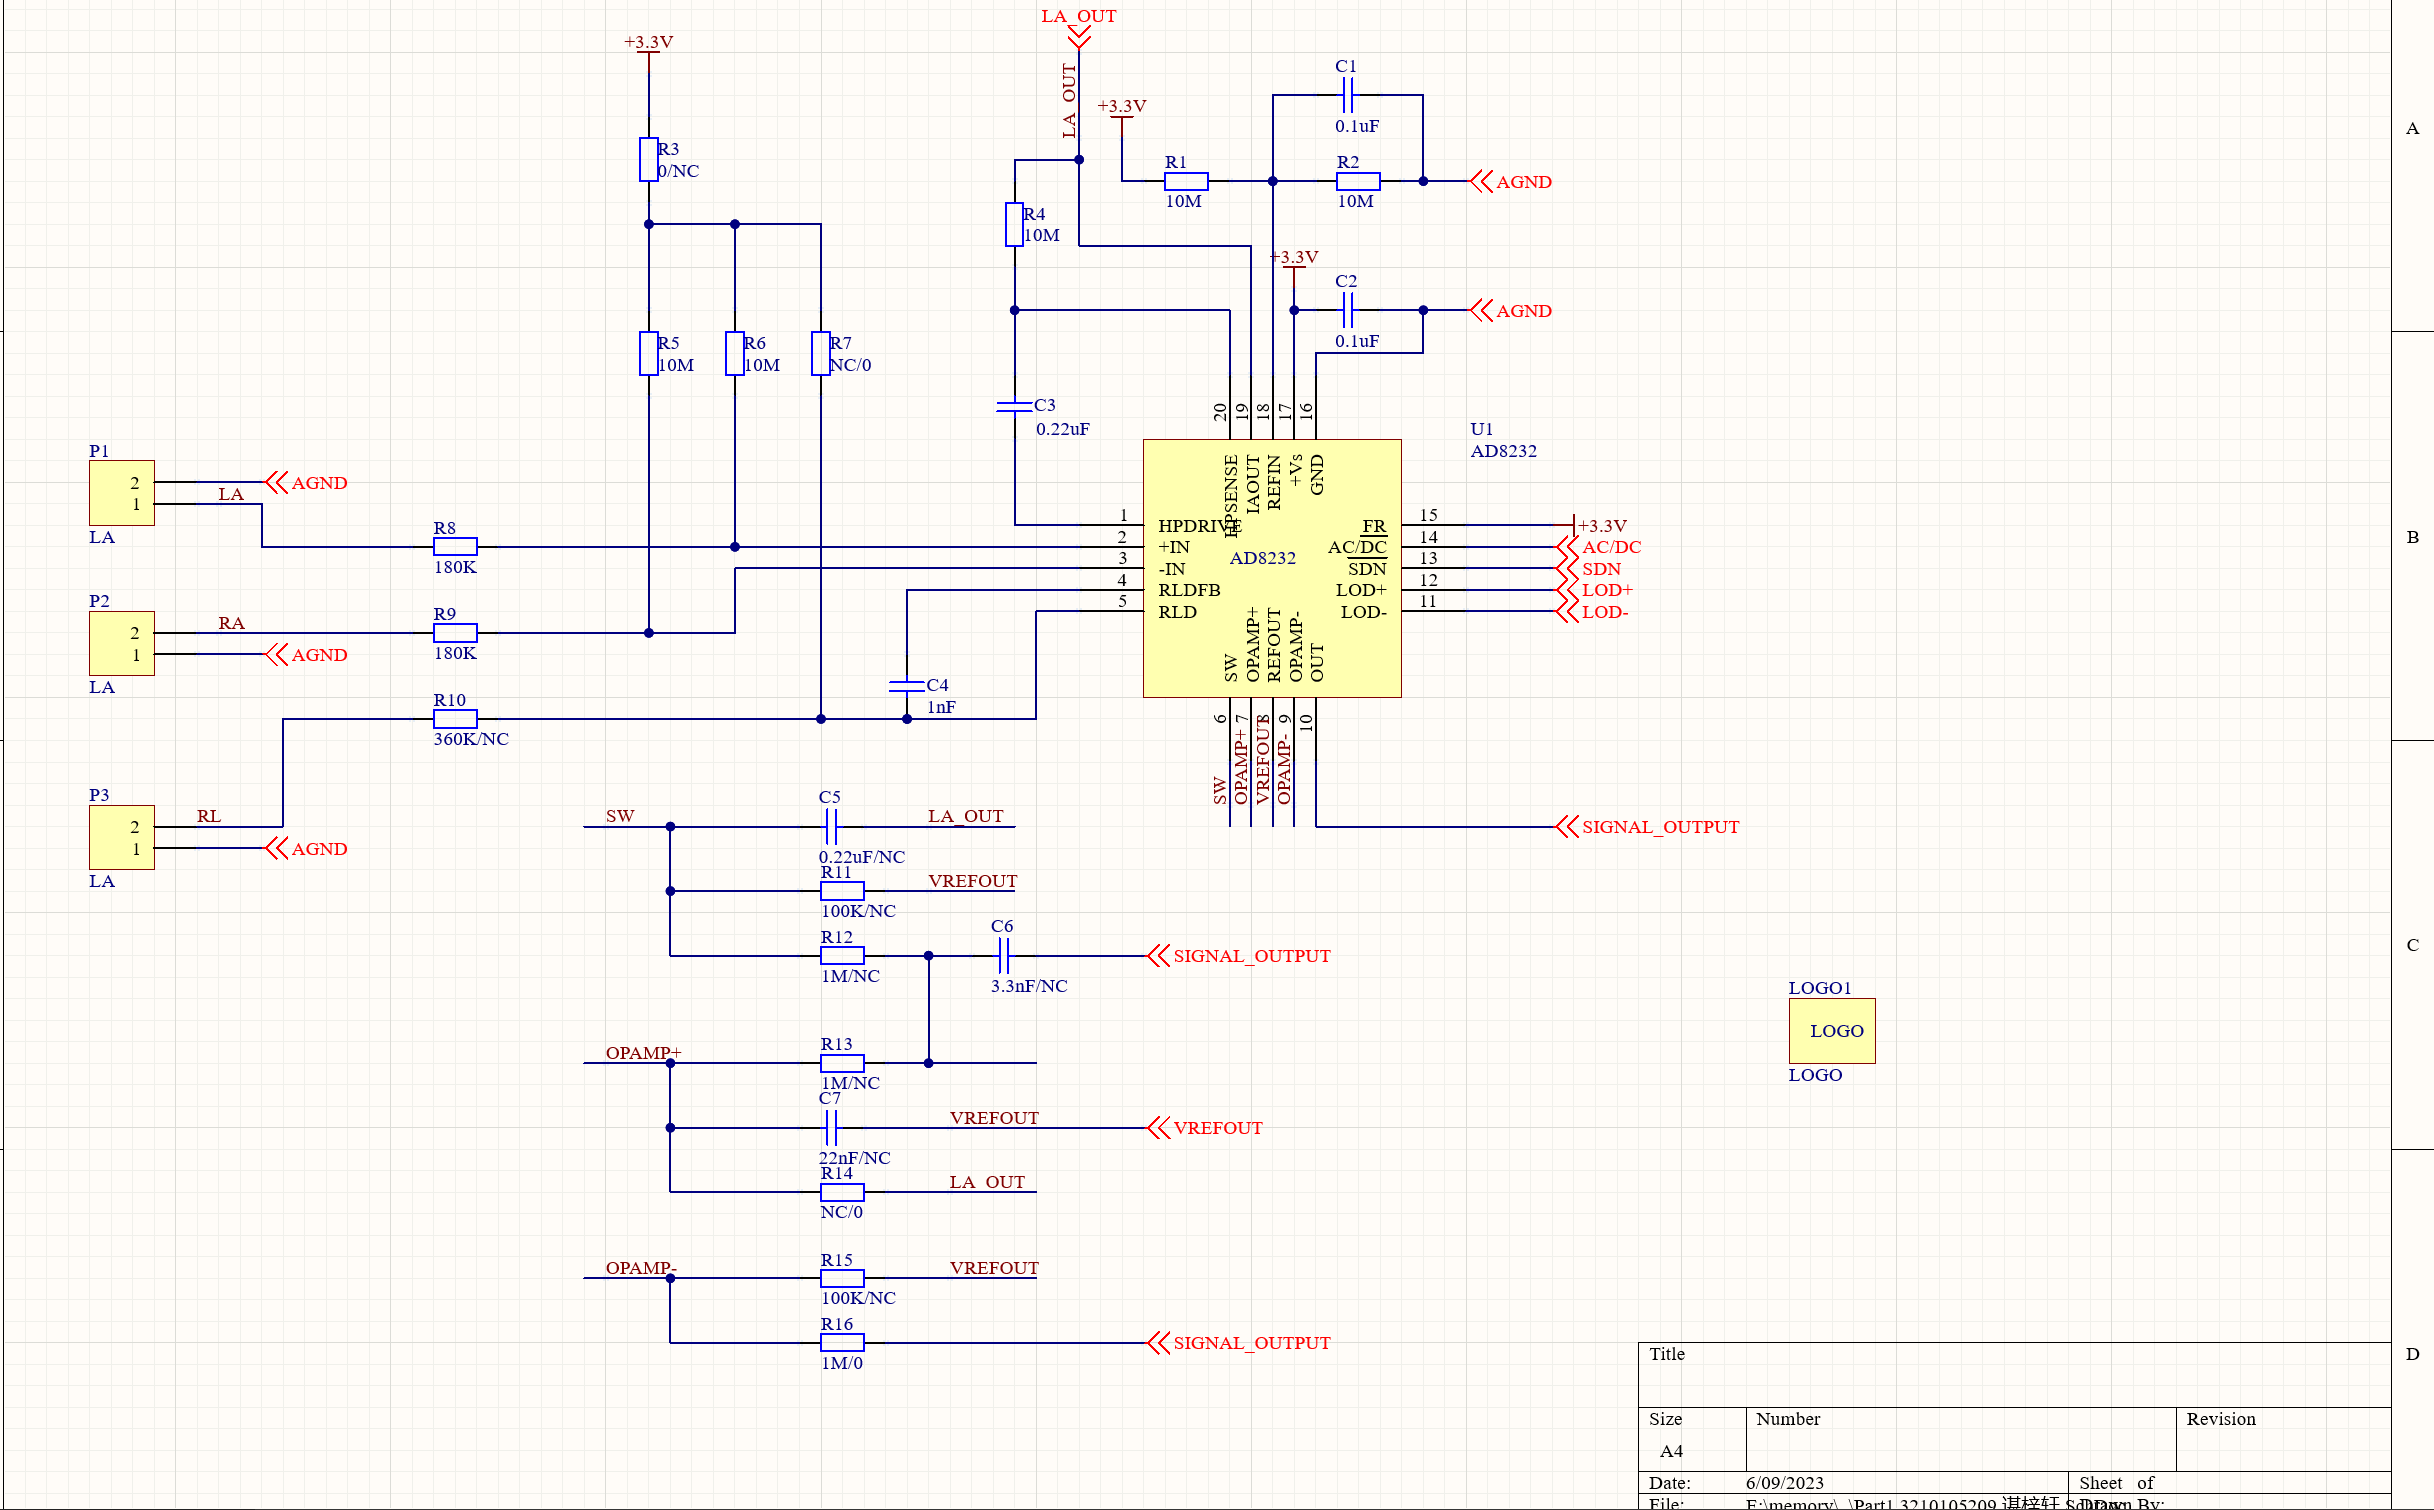
\includegraphics[width=0.9\linewidth]{ECG电路原理图_前端信号接收处理部分}%%%%%%%%%note3
			\caption{ECG电路原理图-前端信号接收处理部分}
			\label{ECG电路原理图_前端信号接收处理部分}
		\end{minipage}%
		\begin{minipage}[t]{0.49\linewidth}
			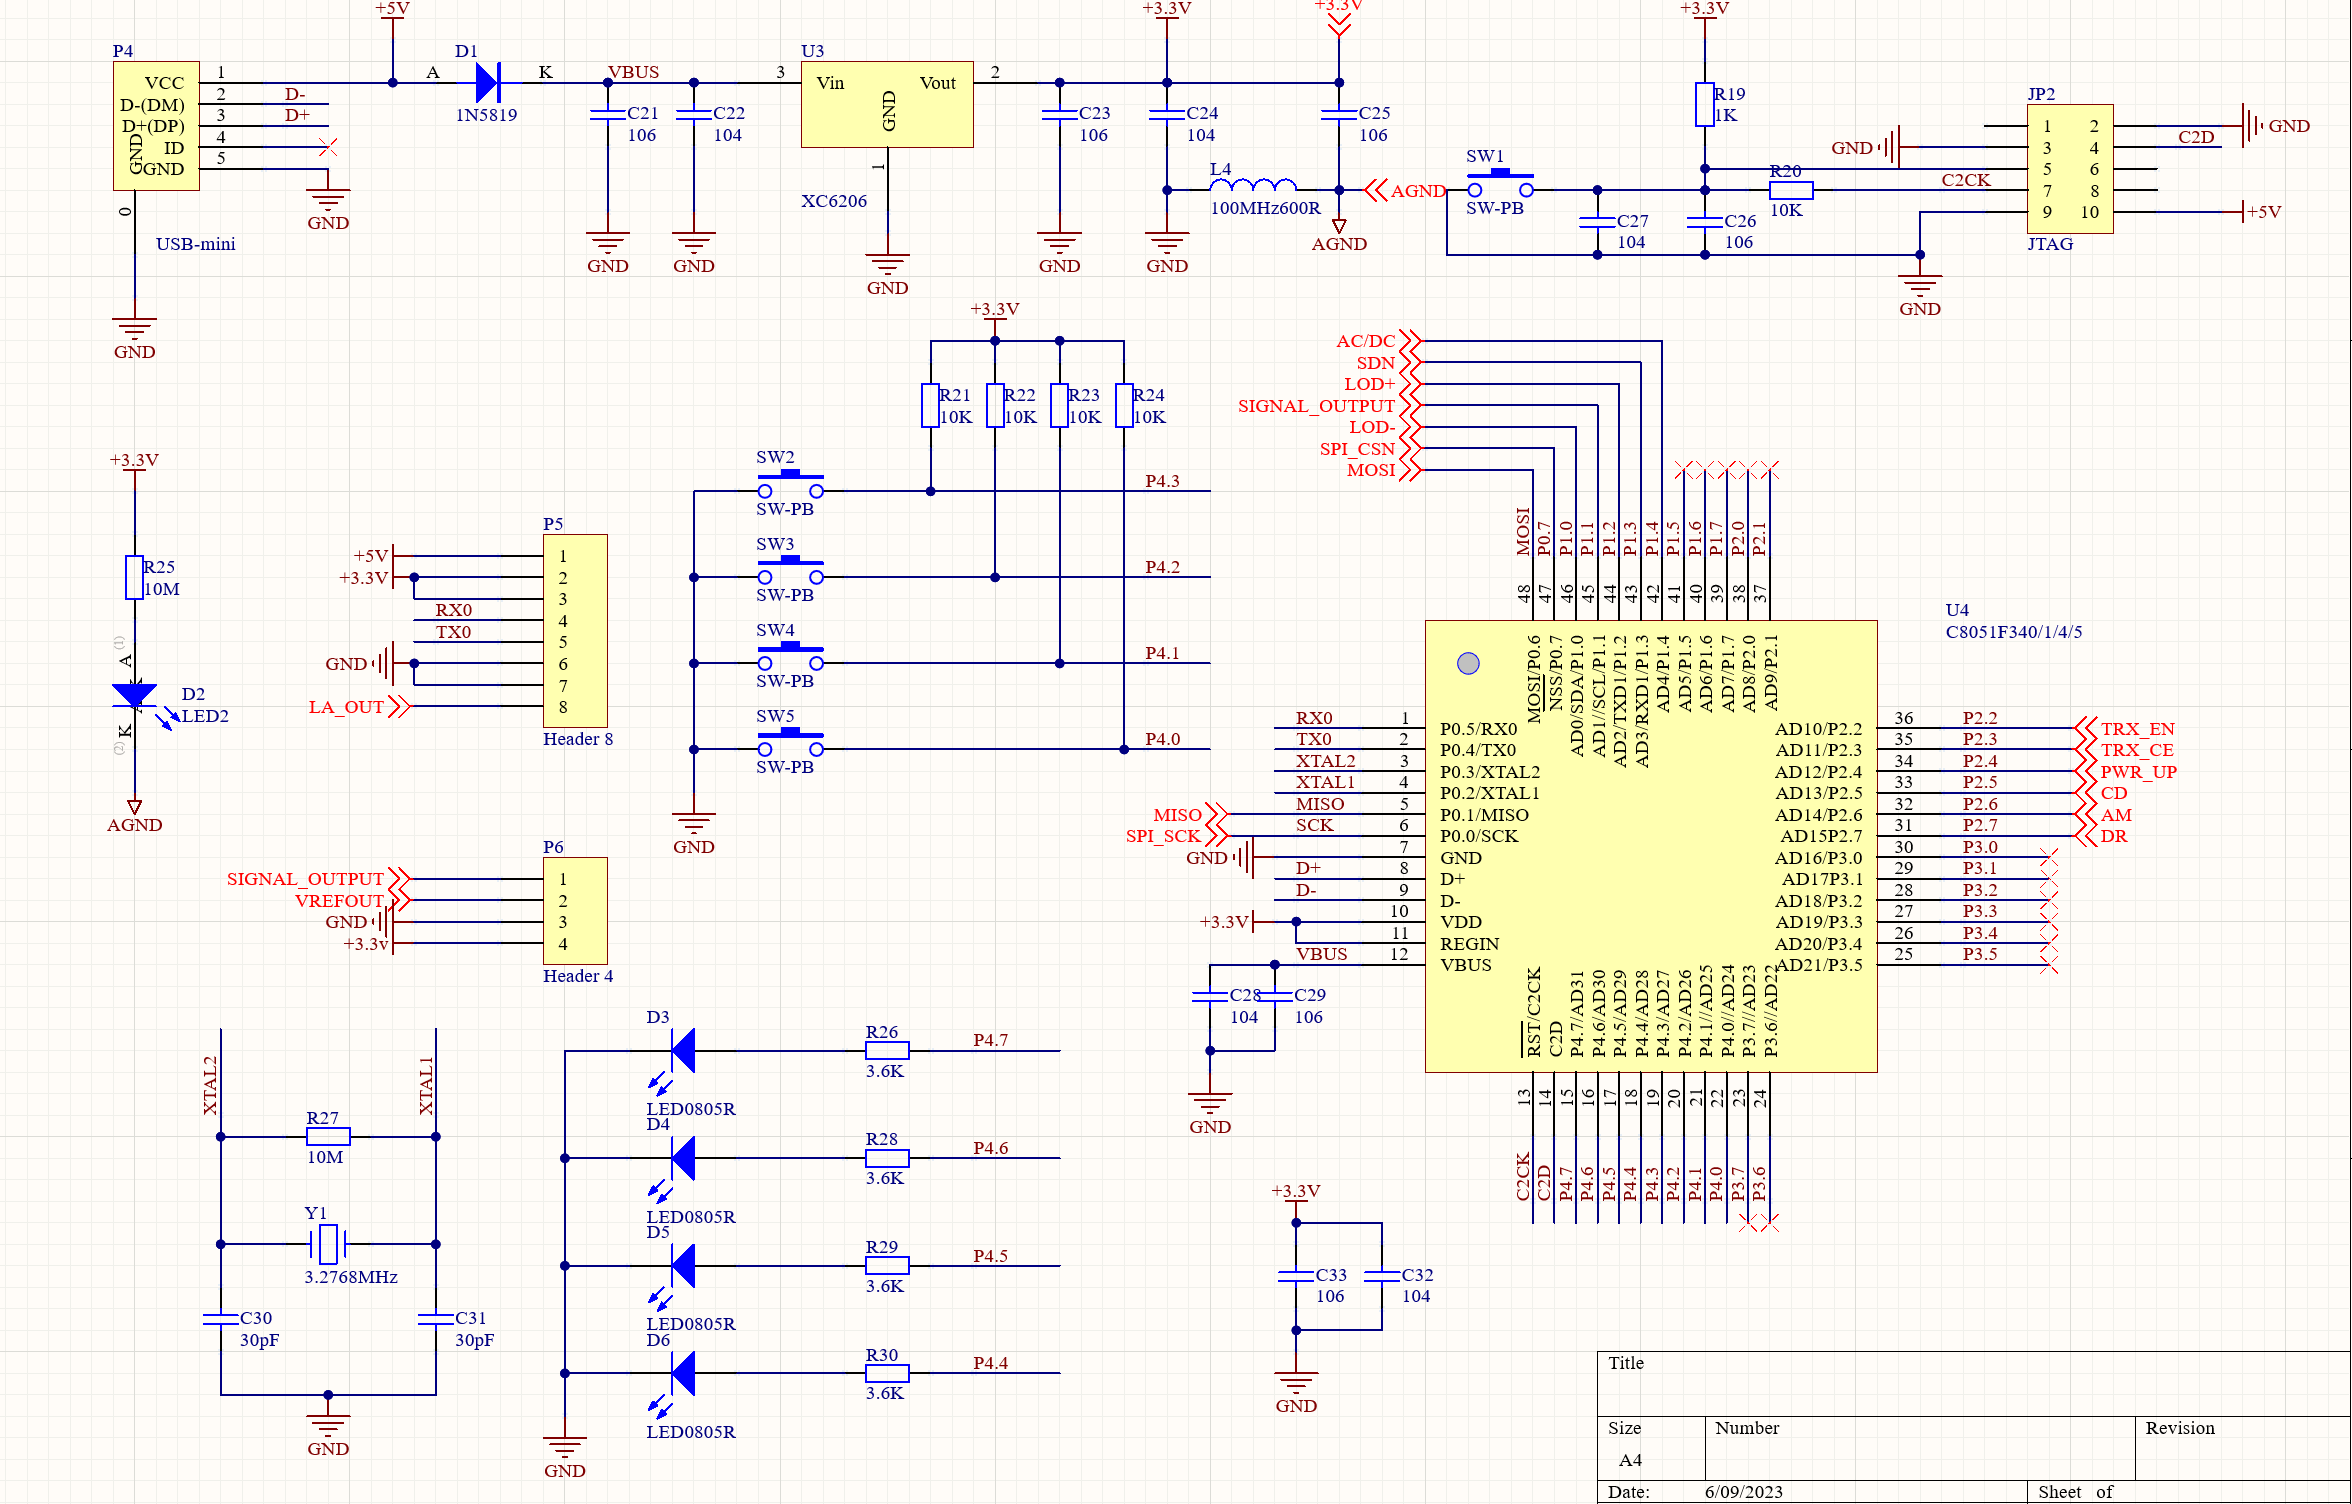
\includegraphics[width=0.9\linewidth]{ECG电路原理图_中间ADC处理部分}
			\caption{ECG电路原理图-中间ADC处理部分}
			\label{ECG电路原理图_中间ADC处理部分}
		\end{minipage}
		
		\begin{minipage}[t]{0.49\linewidth}%%%%%%%%%note2
			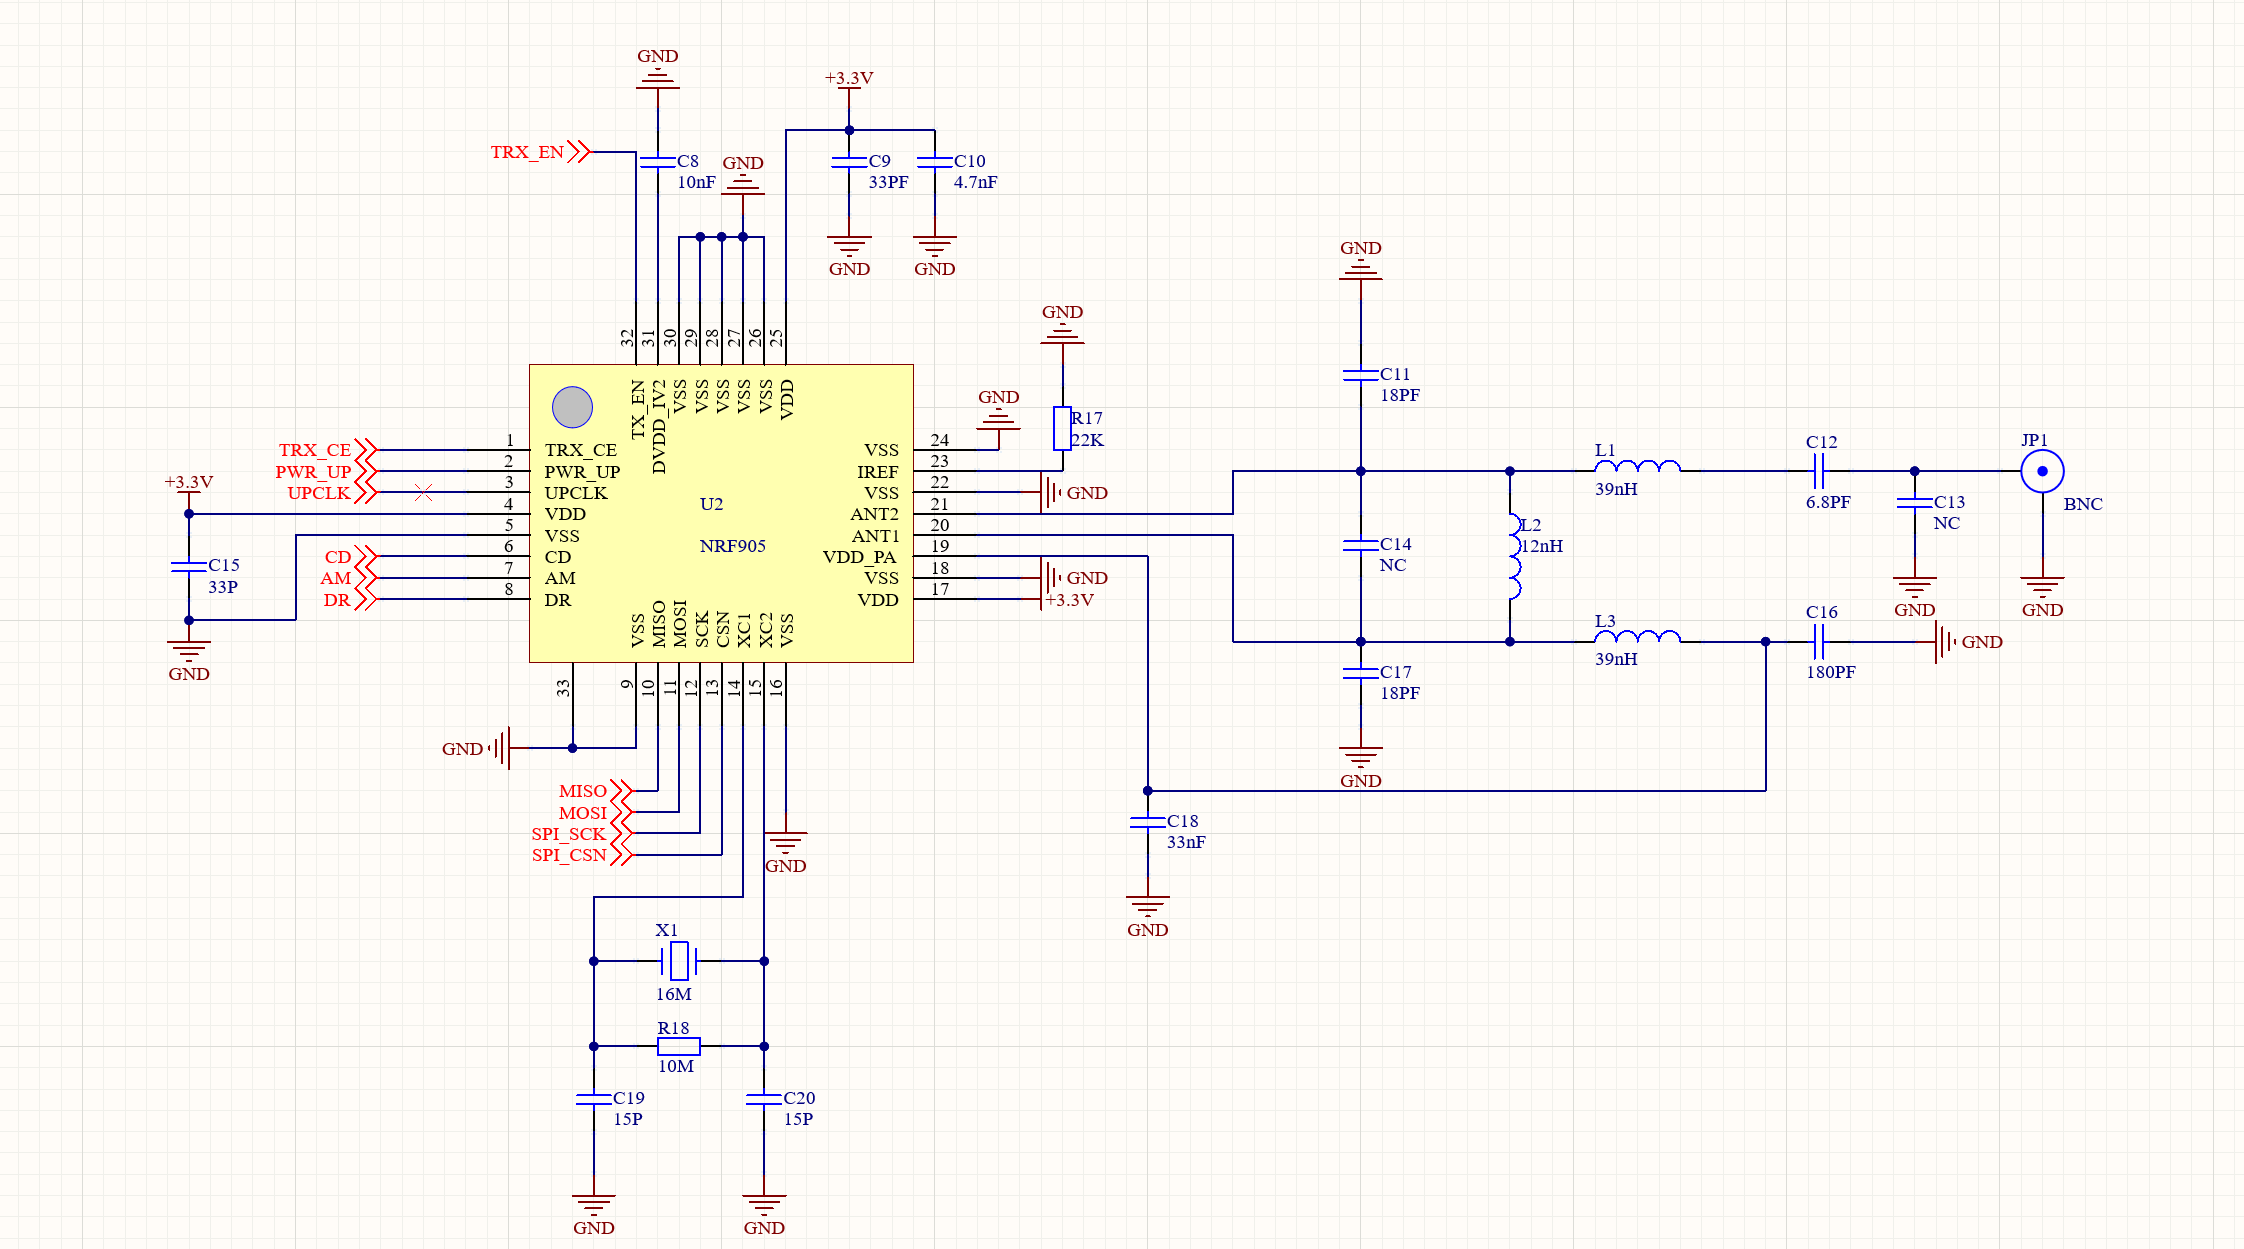
\includegraphics[width=0.9\linewidth]{ECG电路原理图_后端通信与输出部分}%%%%%%%%%note3
			\caption{ECG电路原理图-后端通信与输出部分}
			\label{ECG电路原理图_后端通信与输出部分}
		\end{minipage}%
	\end{figure}
	
	从原理图中,我们可以看出,每一个模块都集成了一块芯片分别负责不同的功能:AD8232主要用于采集人体心电信号,并对其进行滤波、放大等操作;中间部分的51单片机主要负责将处理的信号进行ADC转换;NRF905主要用于射频收发,进行信号的远程传输。
	
	\subsubsection{PCB设计}
	
	\begin{figure}[H]
		\centering%使该部分内容居中
		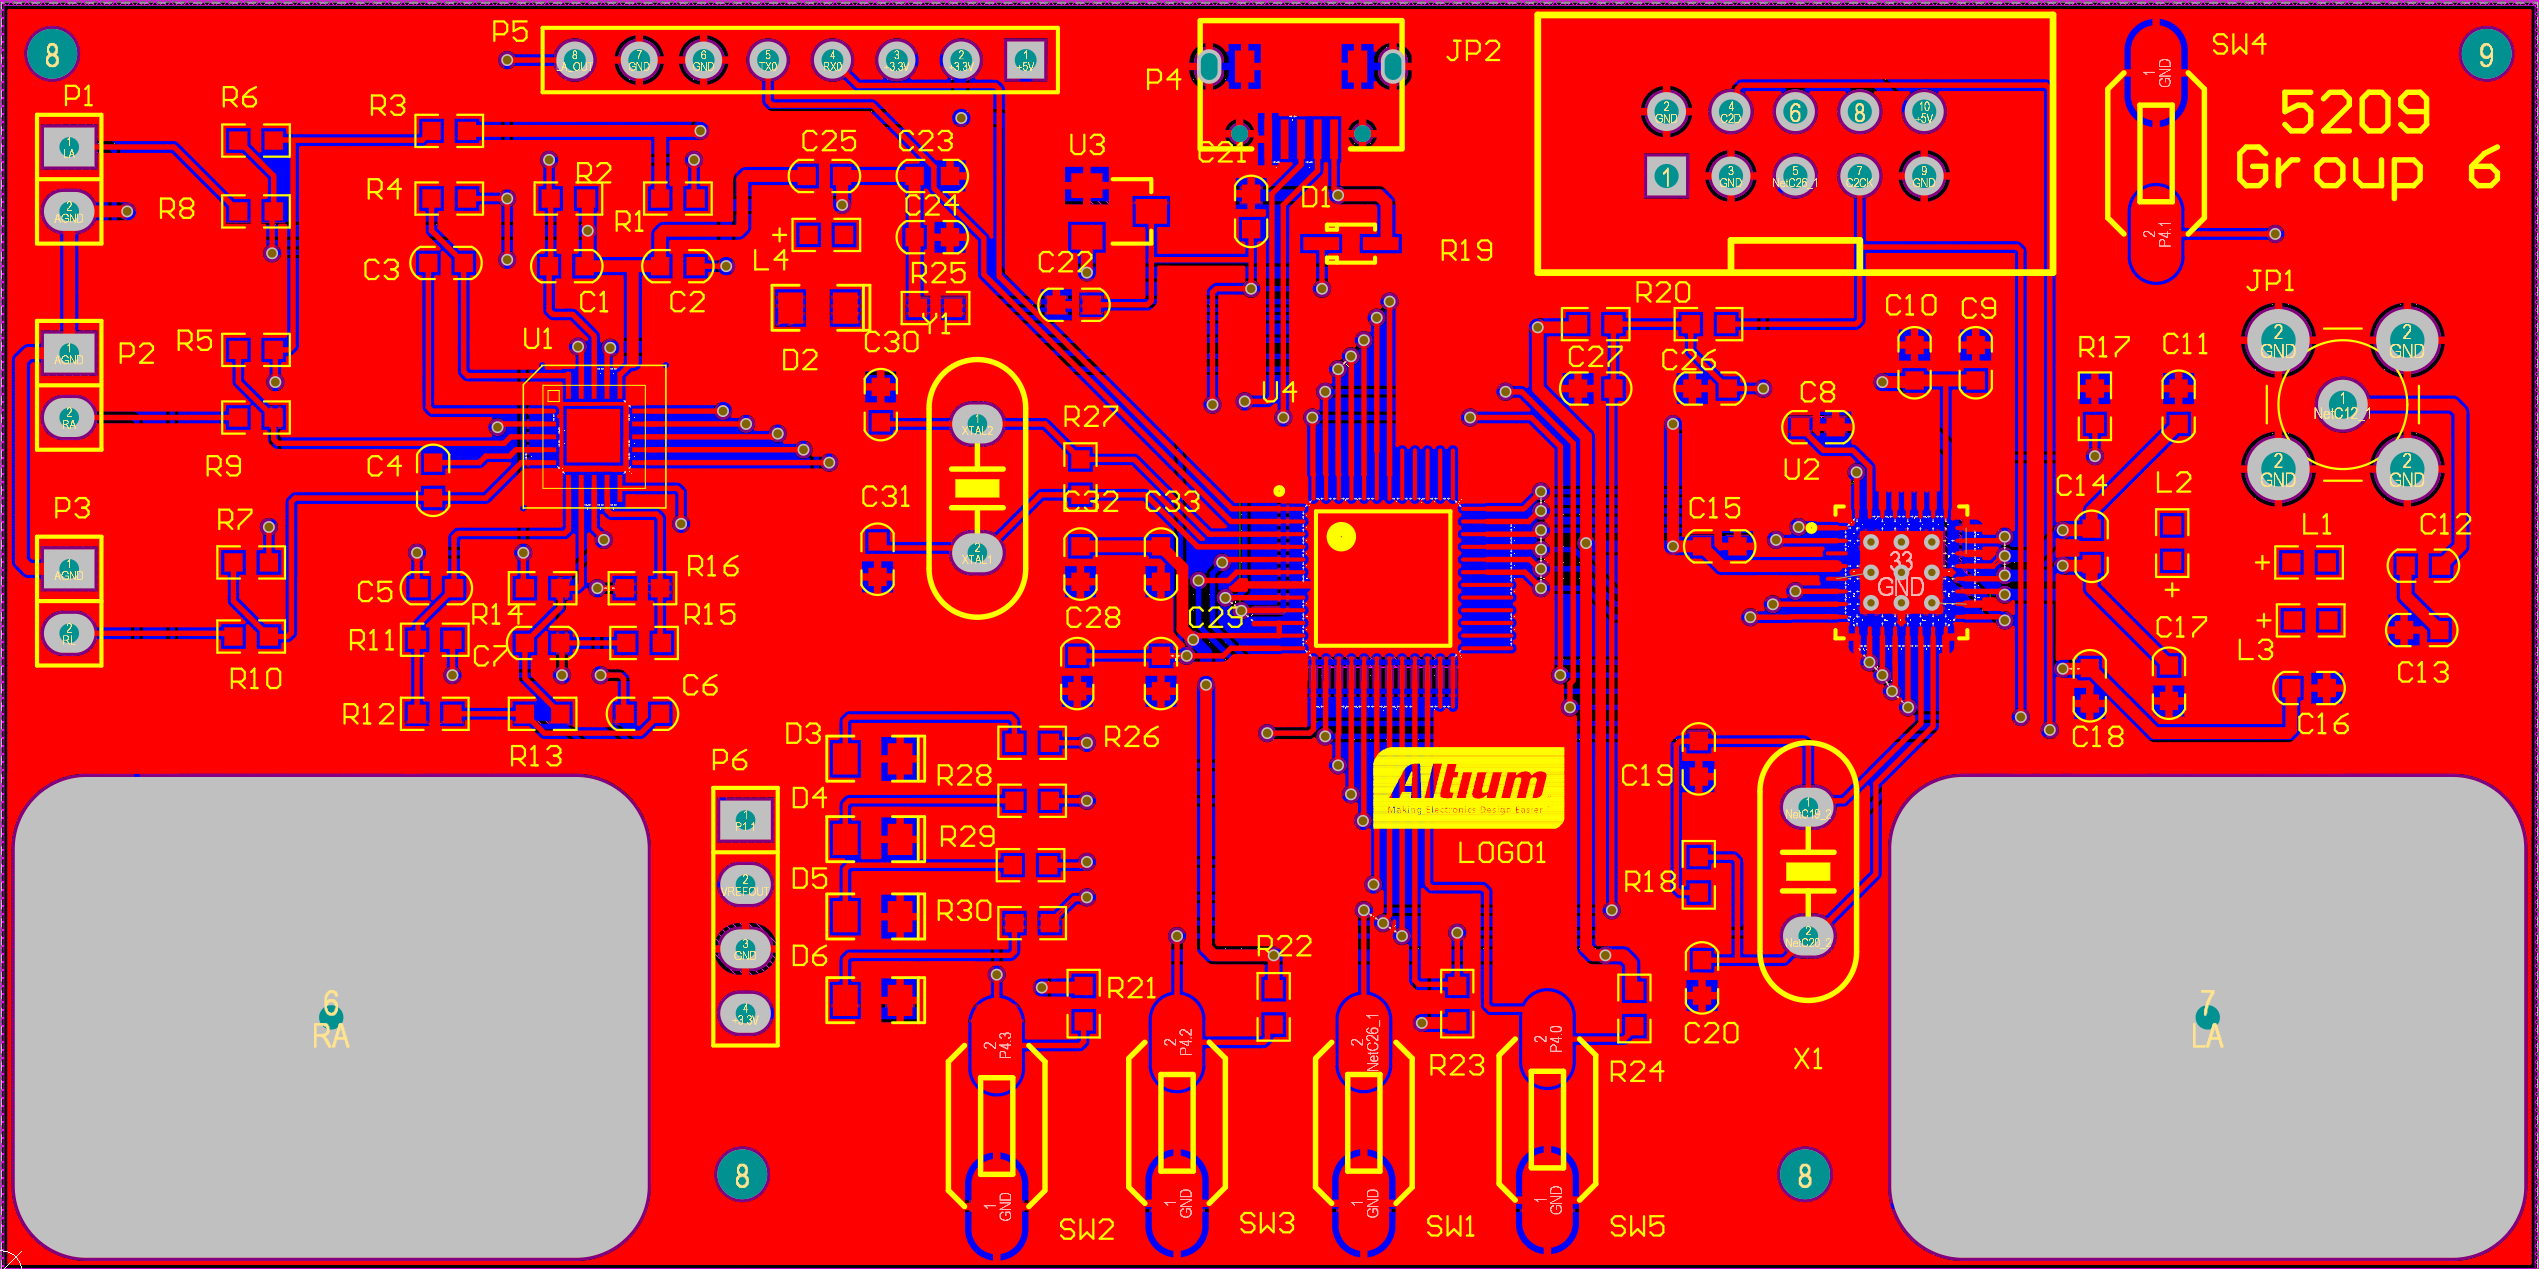
\includegraphics[width=3.5in]{ECG电路PCB图}
		\caption{ECG电路PCB图}%命名并编号
		\label{ECG电路PCB图}%设置标签
	\end{figure}
	
	根据原理图,借助$Altium \quad Designer$软件,生成PCB图,并将元件进行排布、连接和敷铜等操作,最终形成PCB设计图,如图所示。
	
	\subsection{硬件调试}
	
	\subsubsection{共模抑制比}

将信号以差模和共模连接方式分别输入,频率为20Hz,差模信号输入幅度为5mVp-p,共模信号输入幅度为1000mVp-p,右脚驱动作为公共端,将输出信号接到示波器上,可以得到如图\ref{共模输入}、\ref{差模输入}所示的波形结果。

\begin{figure}[H]
	\centering
	\begin{minipage}[t]{0.49\linewidth}%%%%%%%%%note2
		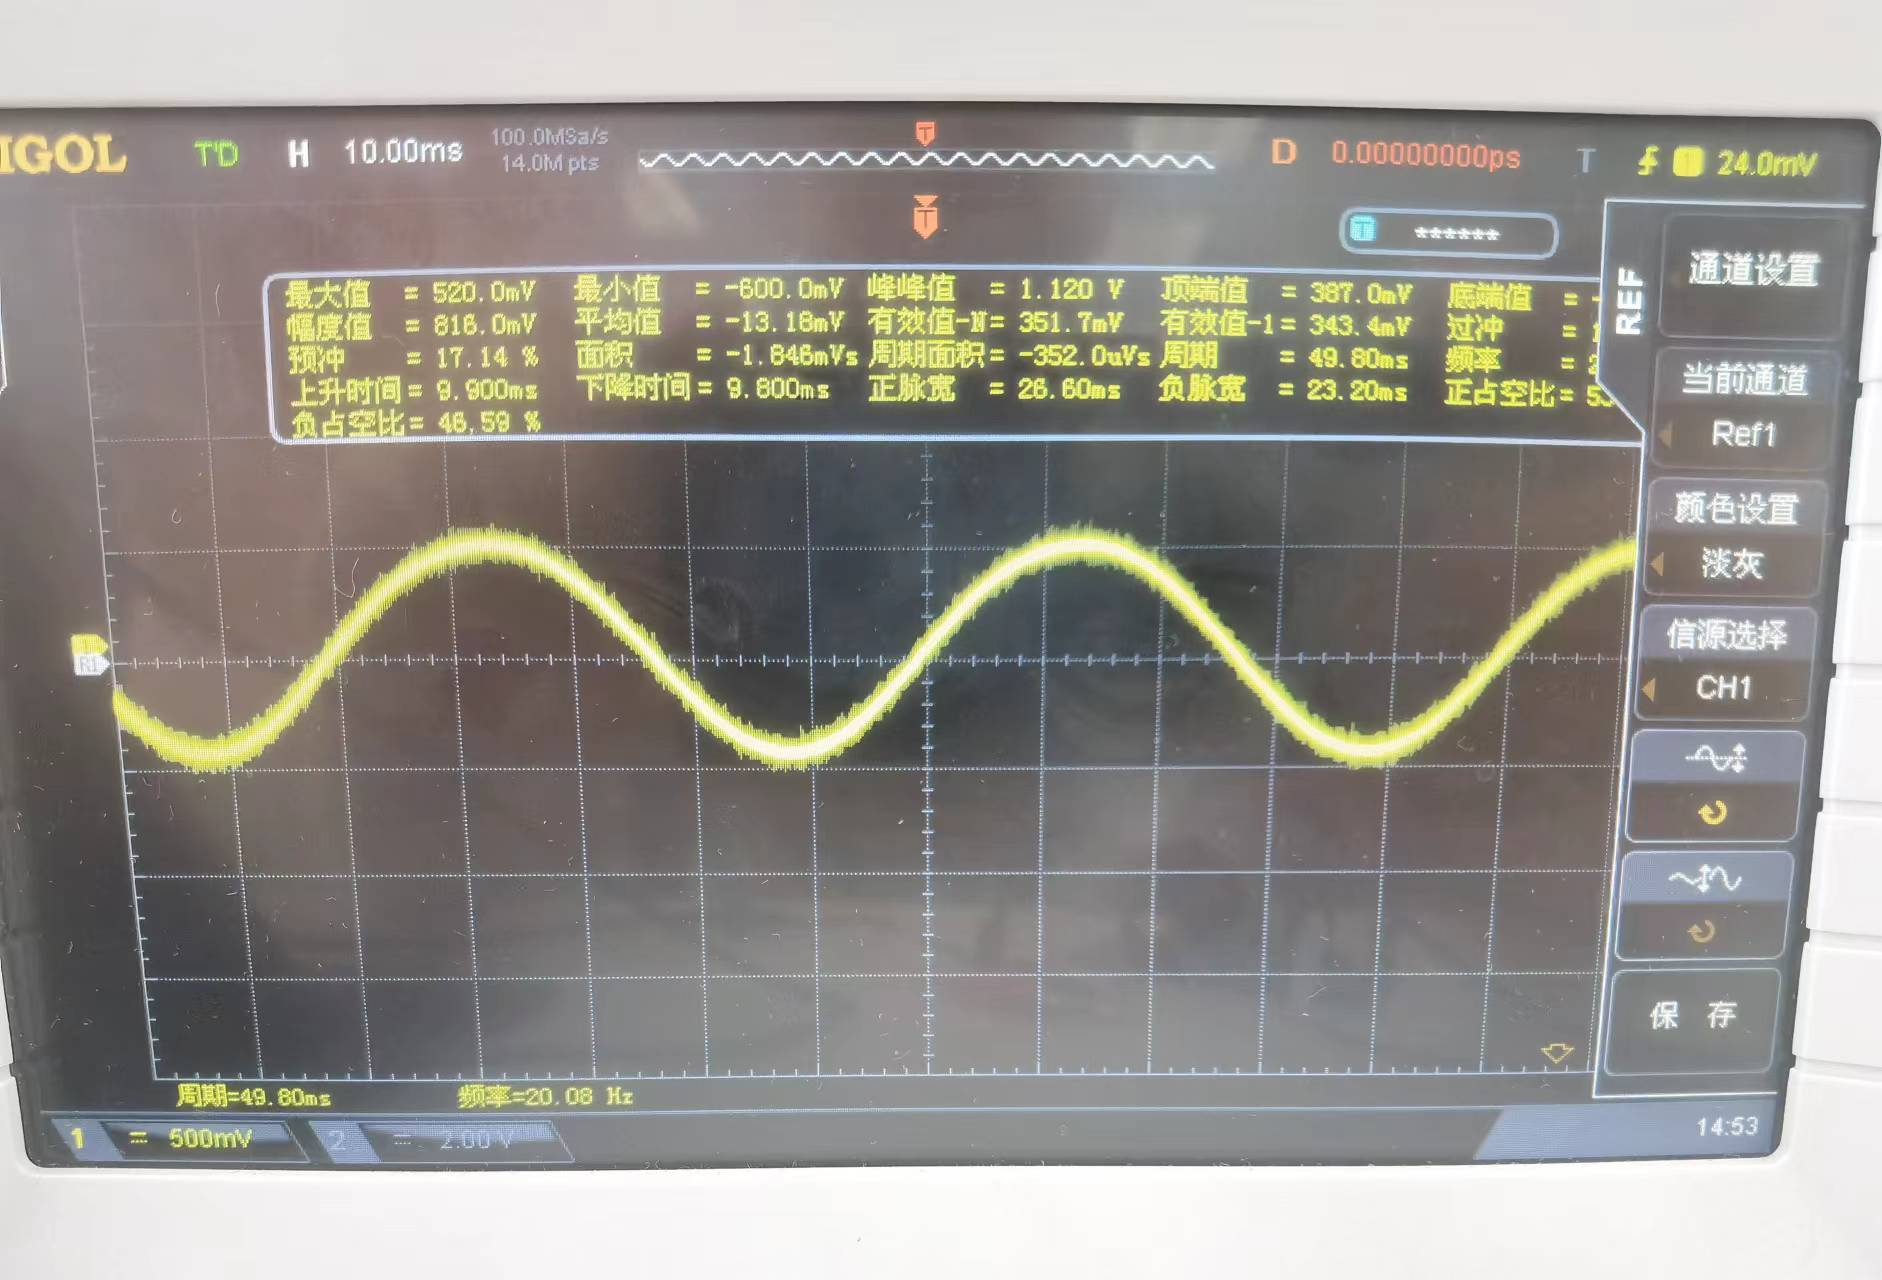
\includegraphics[width=0.9\linewidth]{共模输入}%%%%%%%%%note3
		\caption{共模输入}
		\label{共模输入}
	\end{minipage}%
	\begin{minipage}[t]{0.49\linewidth}
		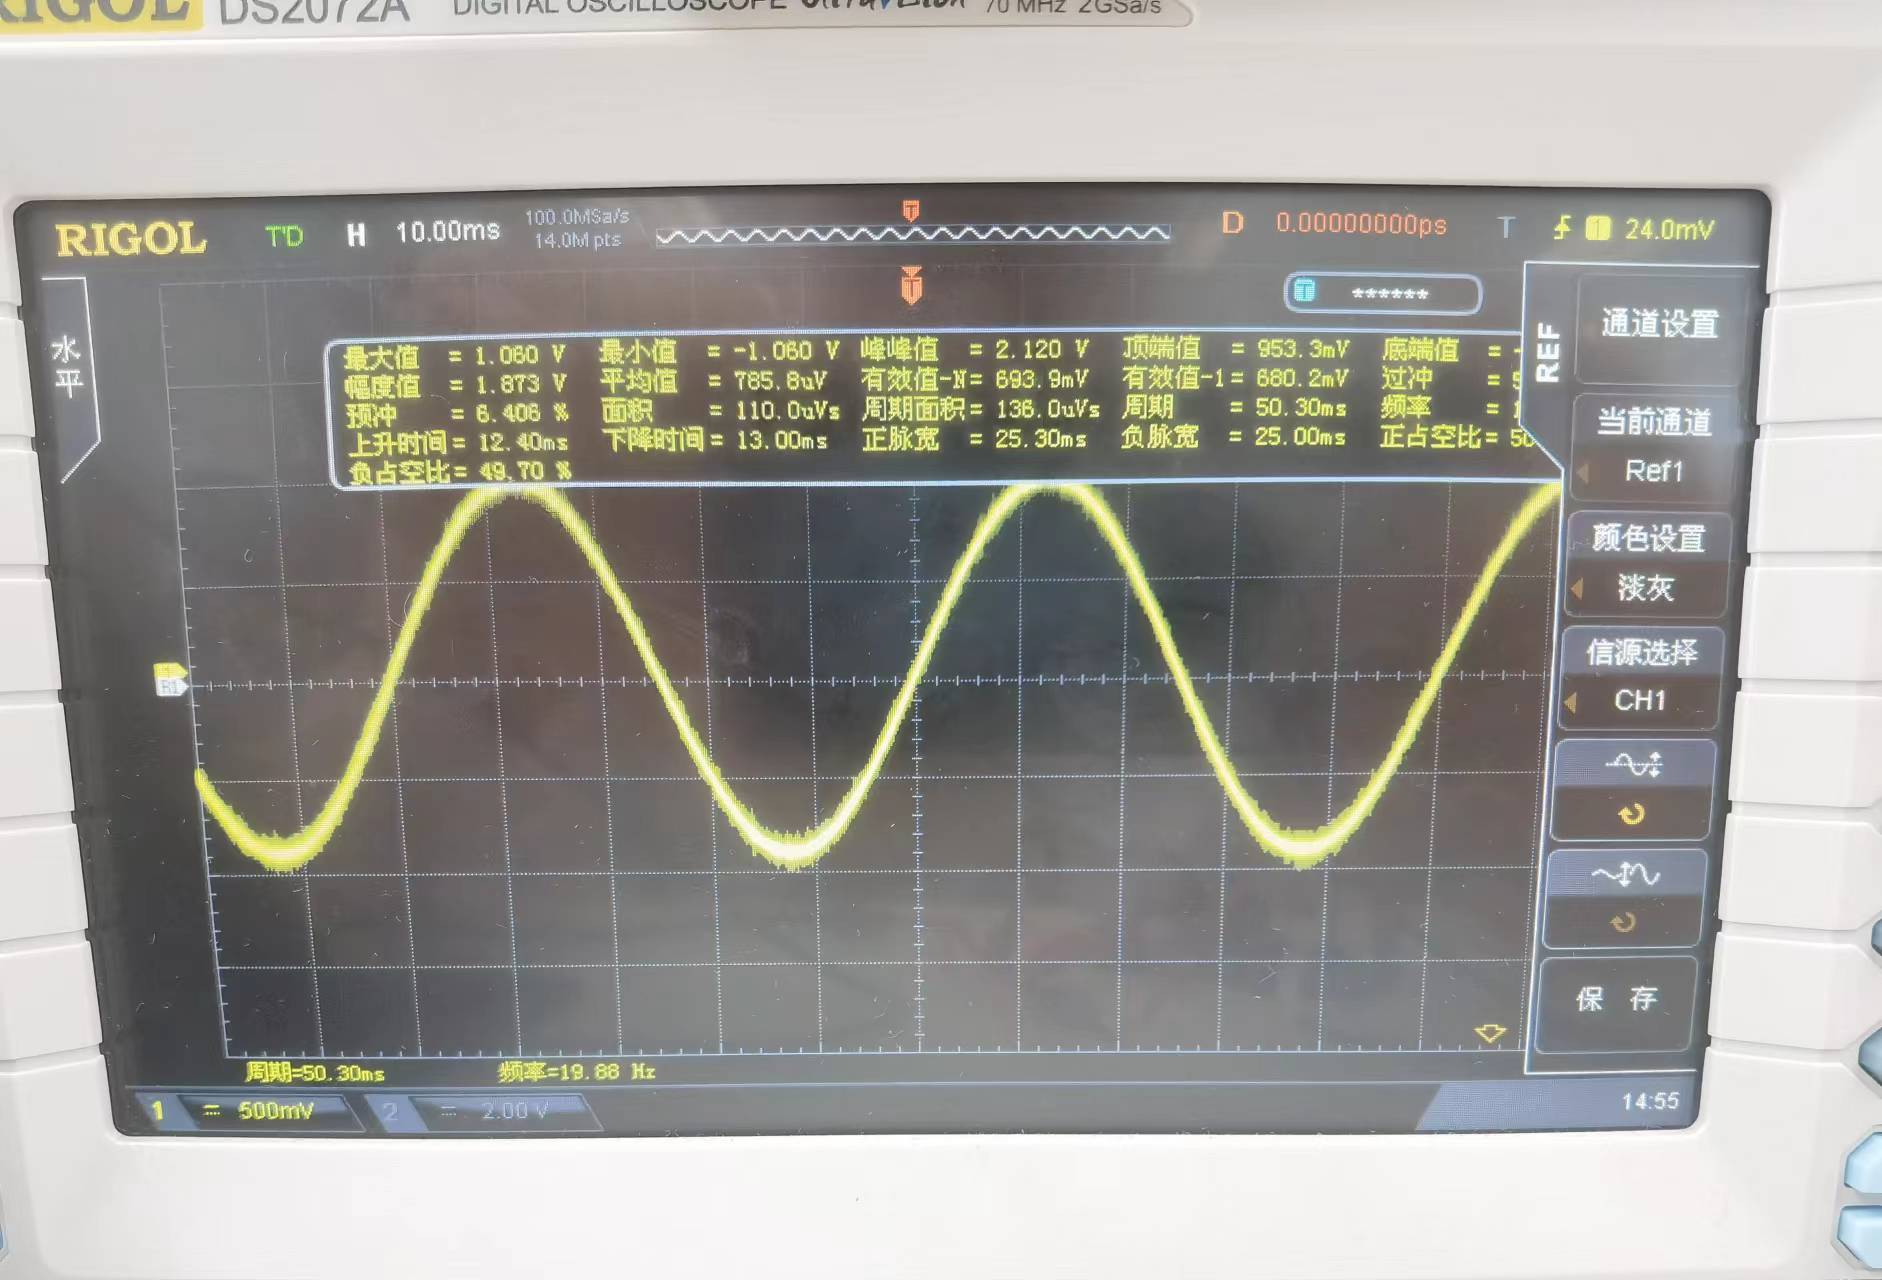
\includegraphics[width=0.9\linewidth]{差模输入}
		\caption{差模输入}
		\label{差模输入}
	\end{minipage}
\end{figure}

从图中我们可以看出,差模增益为420,共模增益为1.12,所以可以算出,共模抑制比为:
\begin{equation}
	CMRR=20\log(\frac{420}{1.12})=51.48dB
\end{equation}
但从CMRR看,共模抑制的效果是不错的,但事实上,可以发现共模部分的增益是大于1的,这主要是由于元件本身质量导致共模抑制的效果不好,且由于杂波信号的毛刺导致测量偏大,故而使得共模增益大于1.

\subsubsection{差模幅频特性}

信号差模输入并调整合适的输入信号幅度,使得输出不失真,测试频率范围:5Hz-100Hz,输出接入到示波器中,逐步调节输入频率,就可以得到差模幅频特性的大致变化,部分信号输出结果如图\ref{幅频特性40Hz}、\ref{幅频特性80Hz}所示,实验数据如表\ref{差模幅频特性数据}所示。

\begin{figure}[H]
	\centering
	\begin{minipage}[t]{0.49\linewidth}%%%%%%%%%note2
		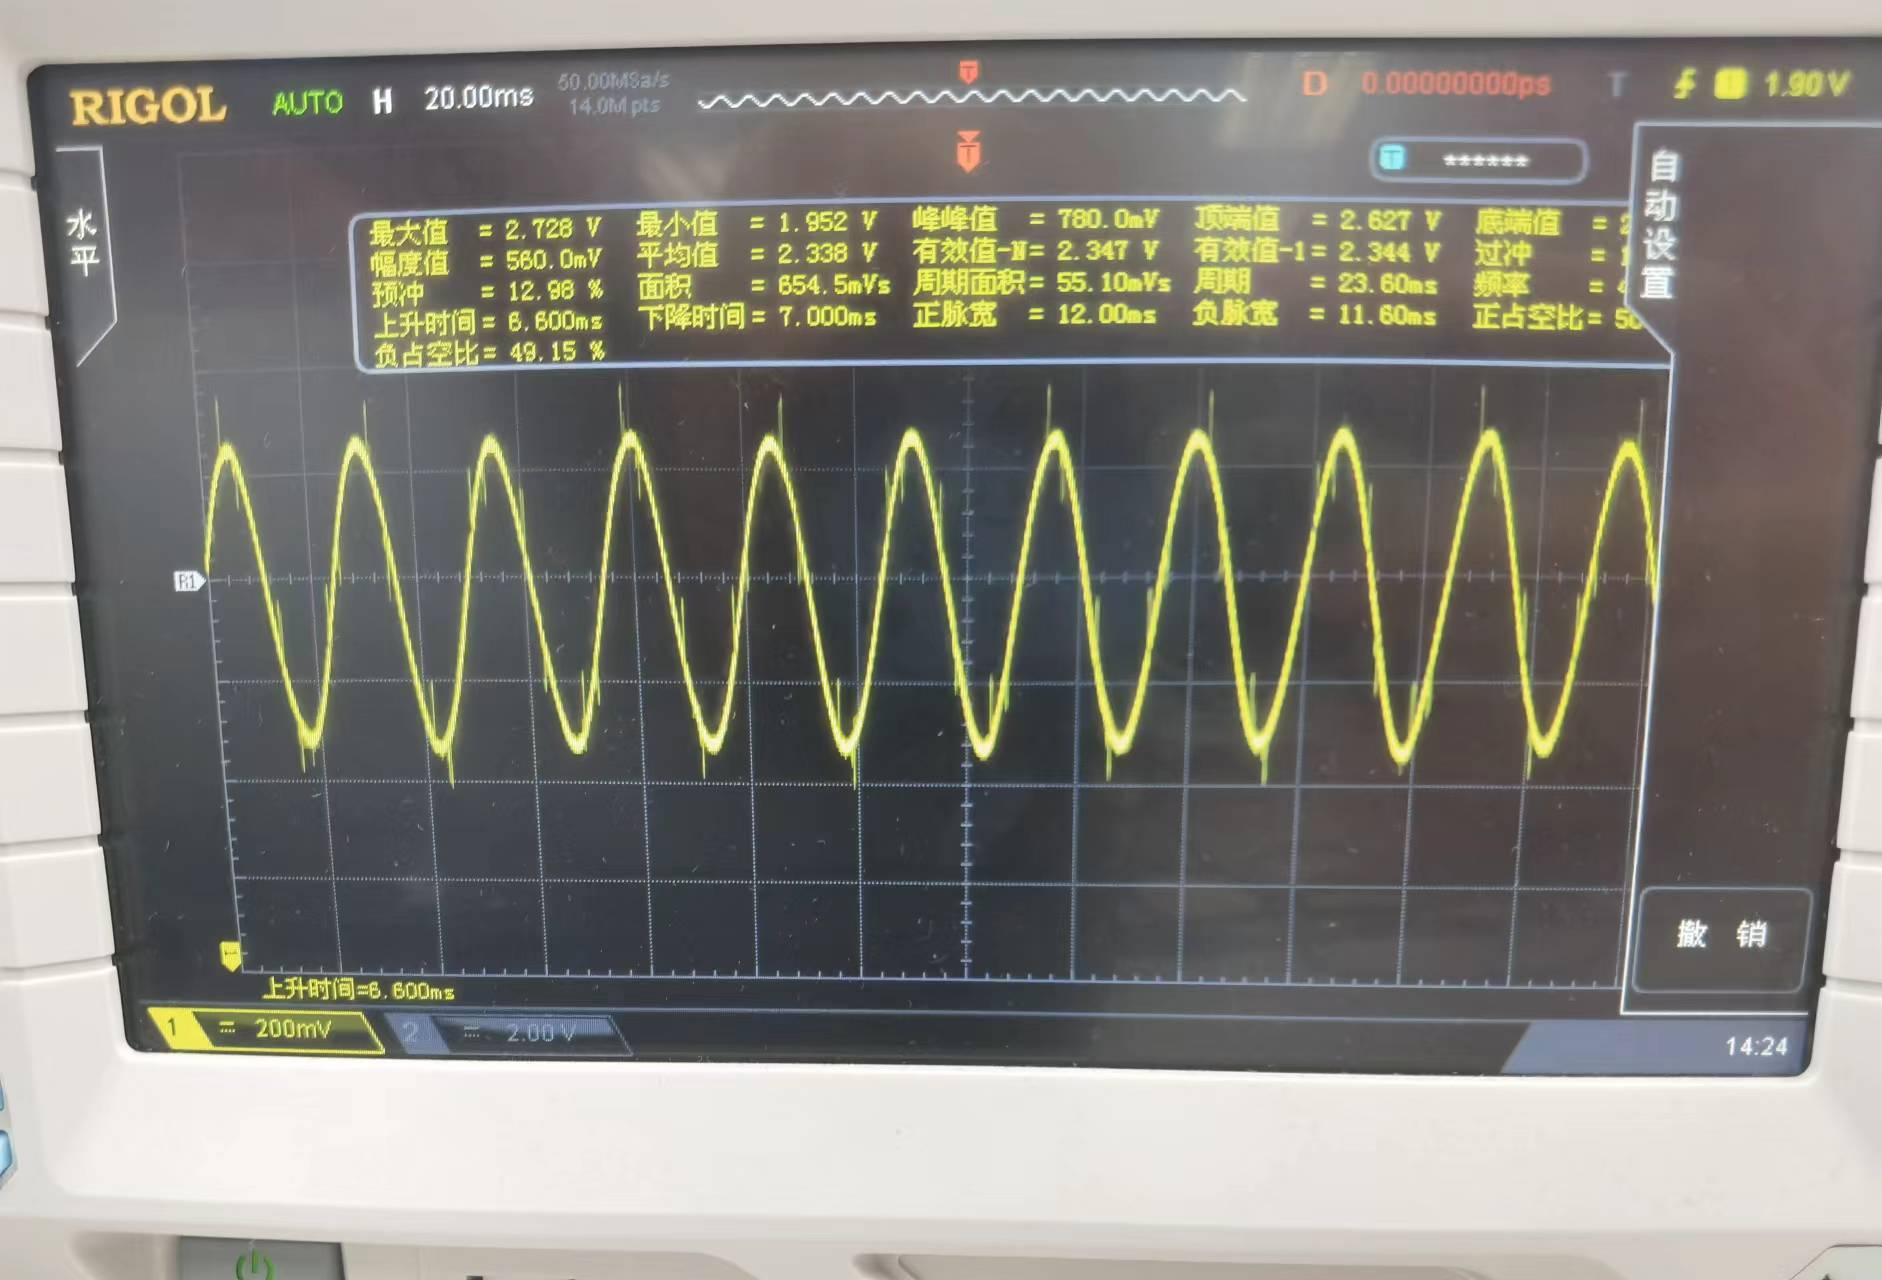
\includegraphics[width=0.9\linewidth]{幅频特性40Hz}%%%%%%%%%note3
		\caption{幅频特性40Hz}
		\label{幅频特性40Hz}
	\end{minipage}%
	\begin{minipage}[t]{0.49\linewidth}
		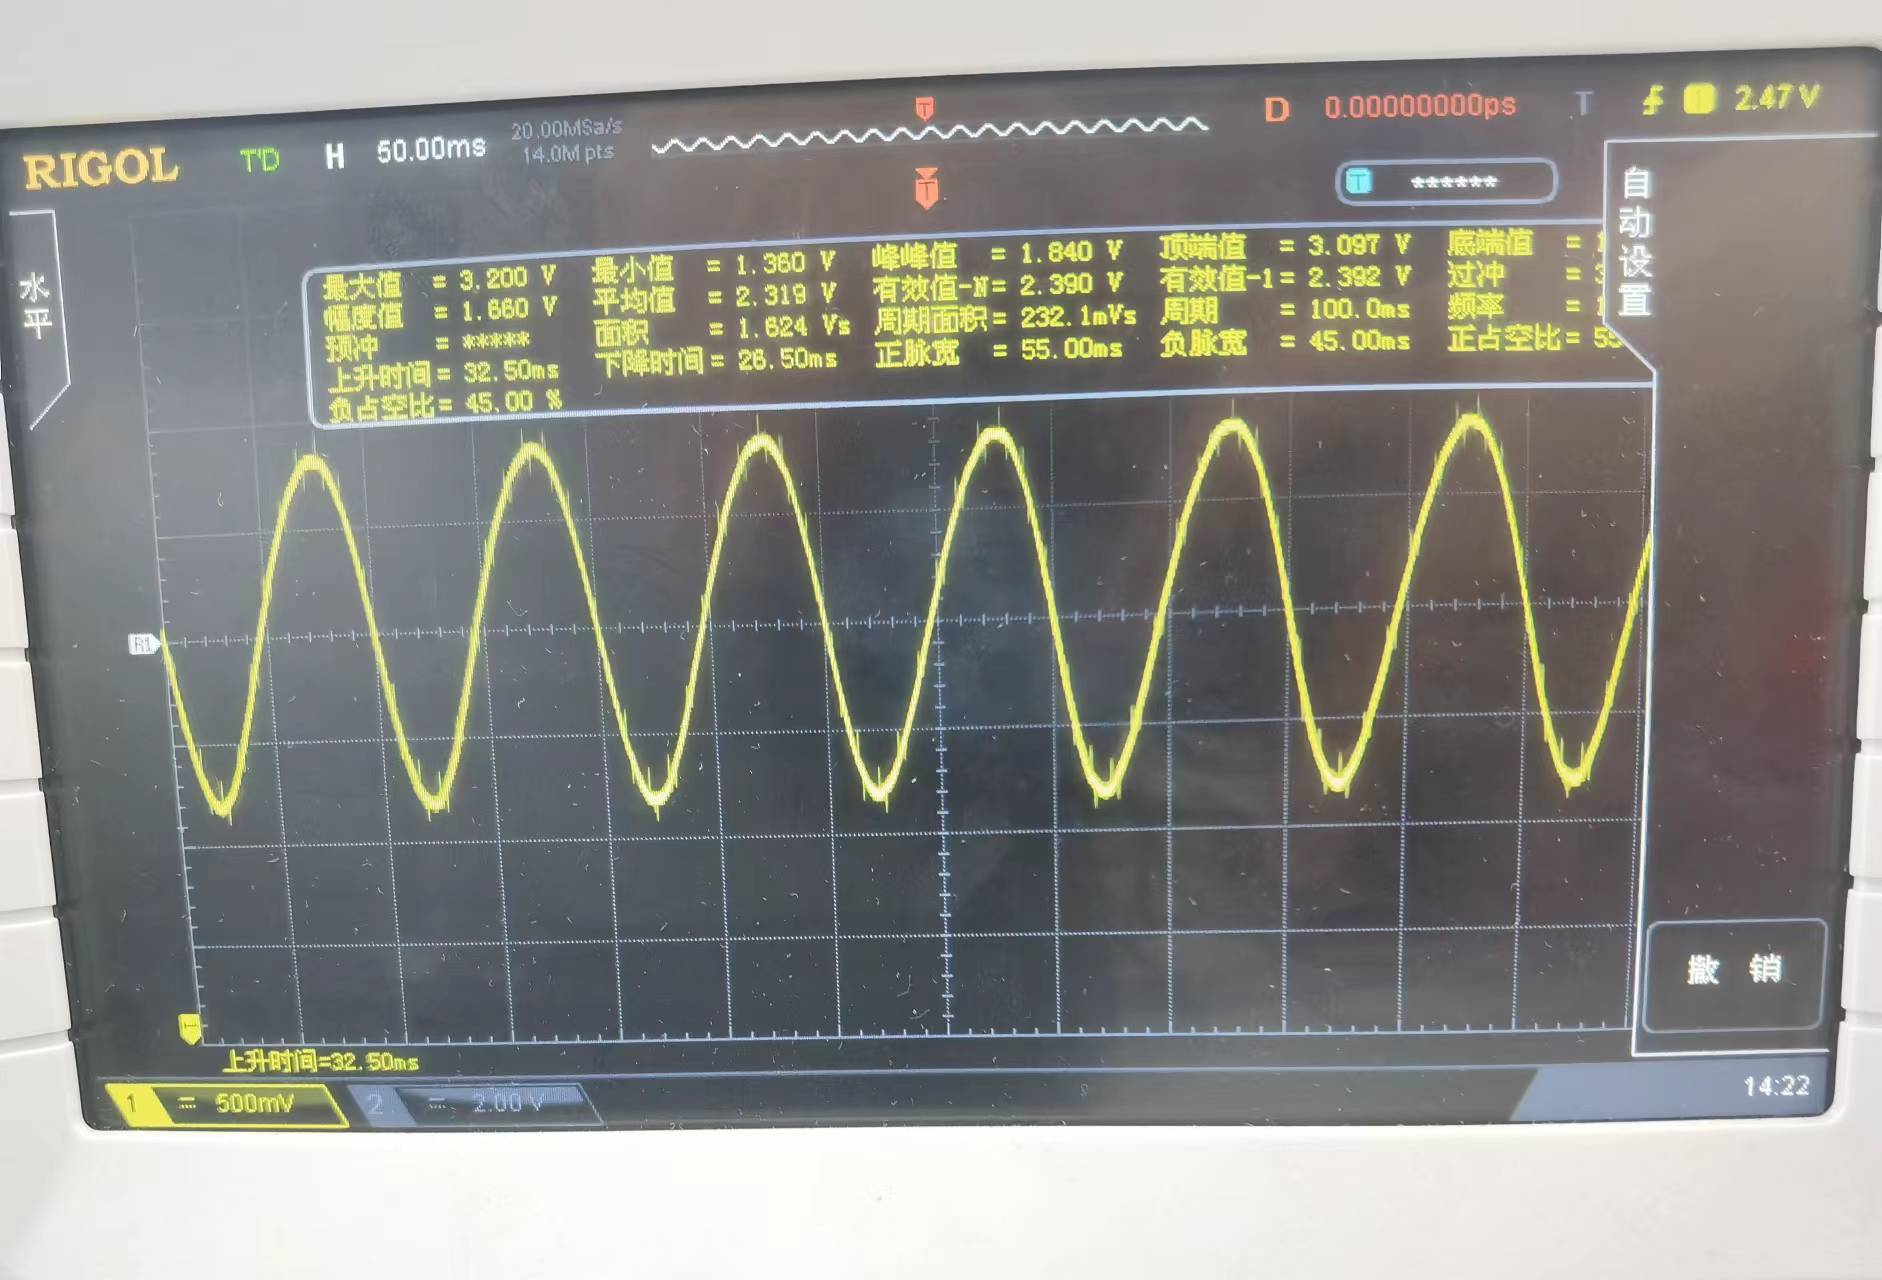
\includegraphics[width=0.9\linewidth]{幅频特性80Hz}
		\caption{幅频特性80Hz}
		\label{幅频特性80Hz}
	\end{minipage}
\end{figure}

\begin{table}[htbp]
	\centering
	\begin{tabular}{ c c c c c c c p{1.5cm}}
		\hline
		频率(mHz) & 5 & 10 & 20 & 40 & 60 & 80 & 100  \\
		\hline
		峰峰值(V)  & 0.230 & 0.350 & 0.450 & 0.780 & 2.100 & 1.840 & 0.920 \\
		\hline
	\end{tabular}
	\caption{差模幅频特性数据}\label{差模幅频特性数据}
\end{table}

根据表中数据,我们可以得到如图\ref{差模幅频特性}所示的幅频特性曲线图,可以看出,随着频率的增大,信号幅度先增大后减小。

\begin{figure}[h]
	\centering%使该部分内容居中
	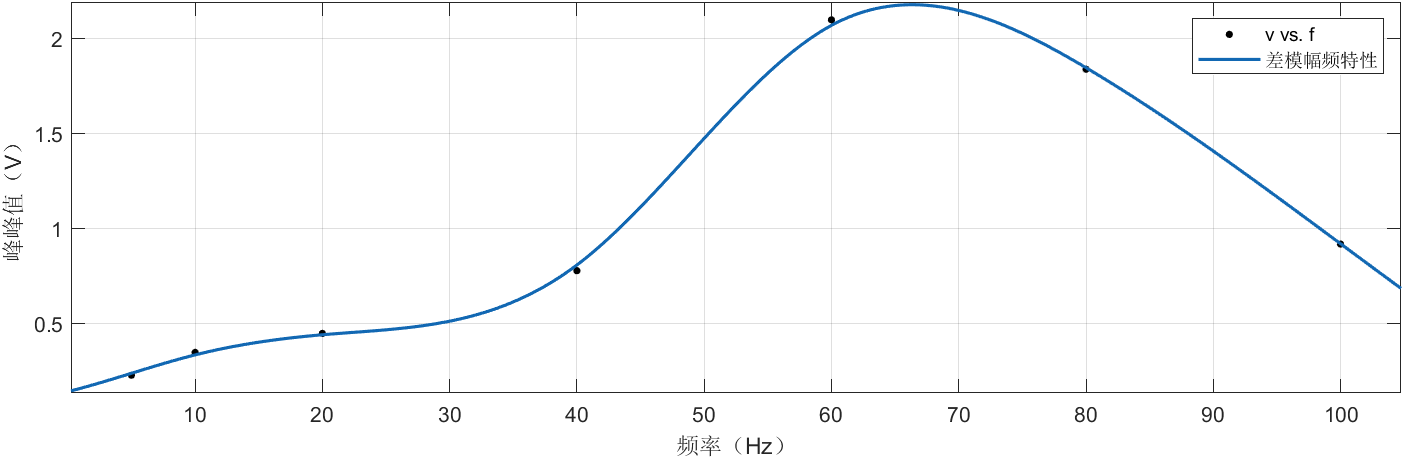
\includegraphics[width=6in]{差模幅频特性}
	\caption{差模幅频特性}%命名并编号
	\label{差模幅频特性}%设置标签
\end{figure}

\subsubsection{脉冲信号波形}

输入信号幅度为5mVp-p、频率为2Hz,占空比为50\%的脉冲波,能够在示波器上得到如图所示的脉冲波信号。

\begin{figure}[h]
	\centering%使该部分内容居中
	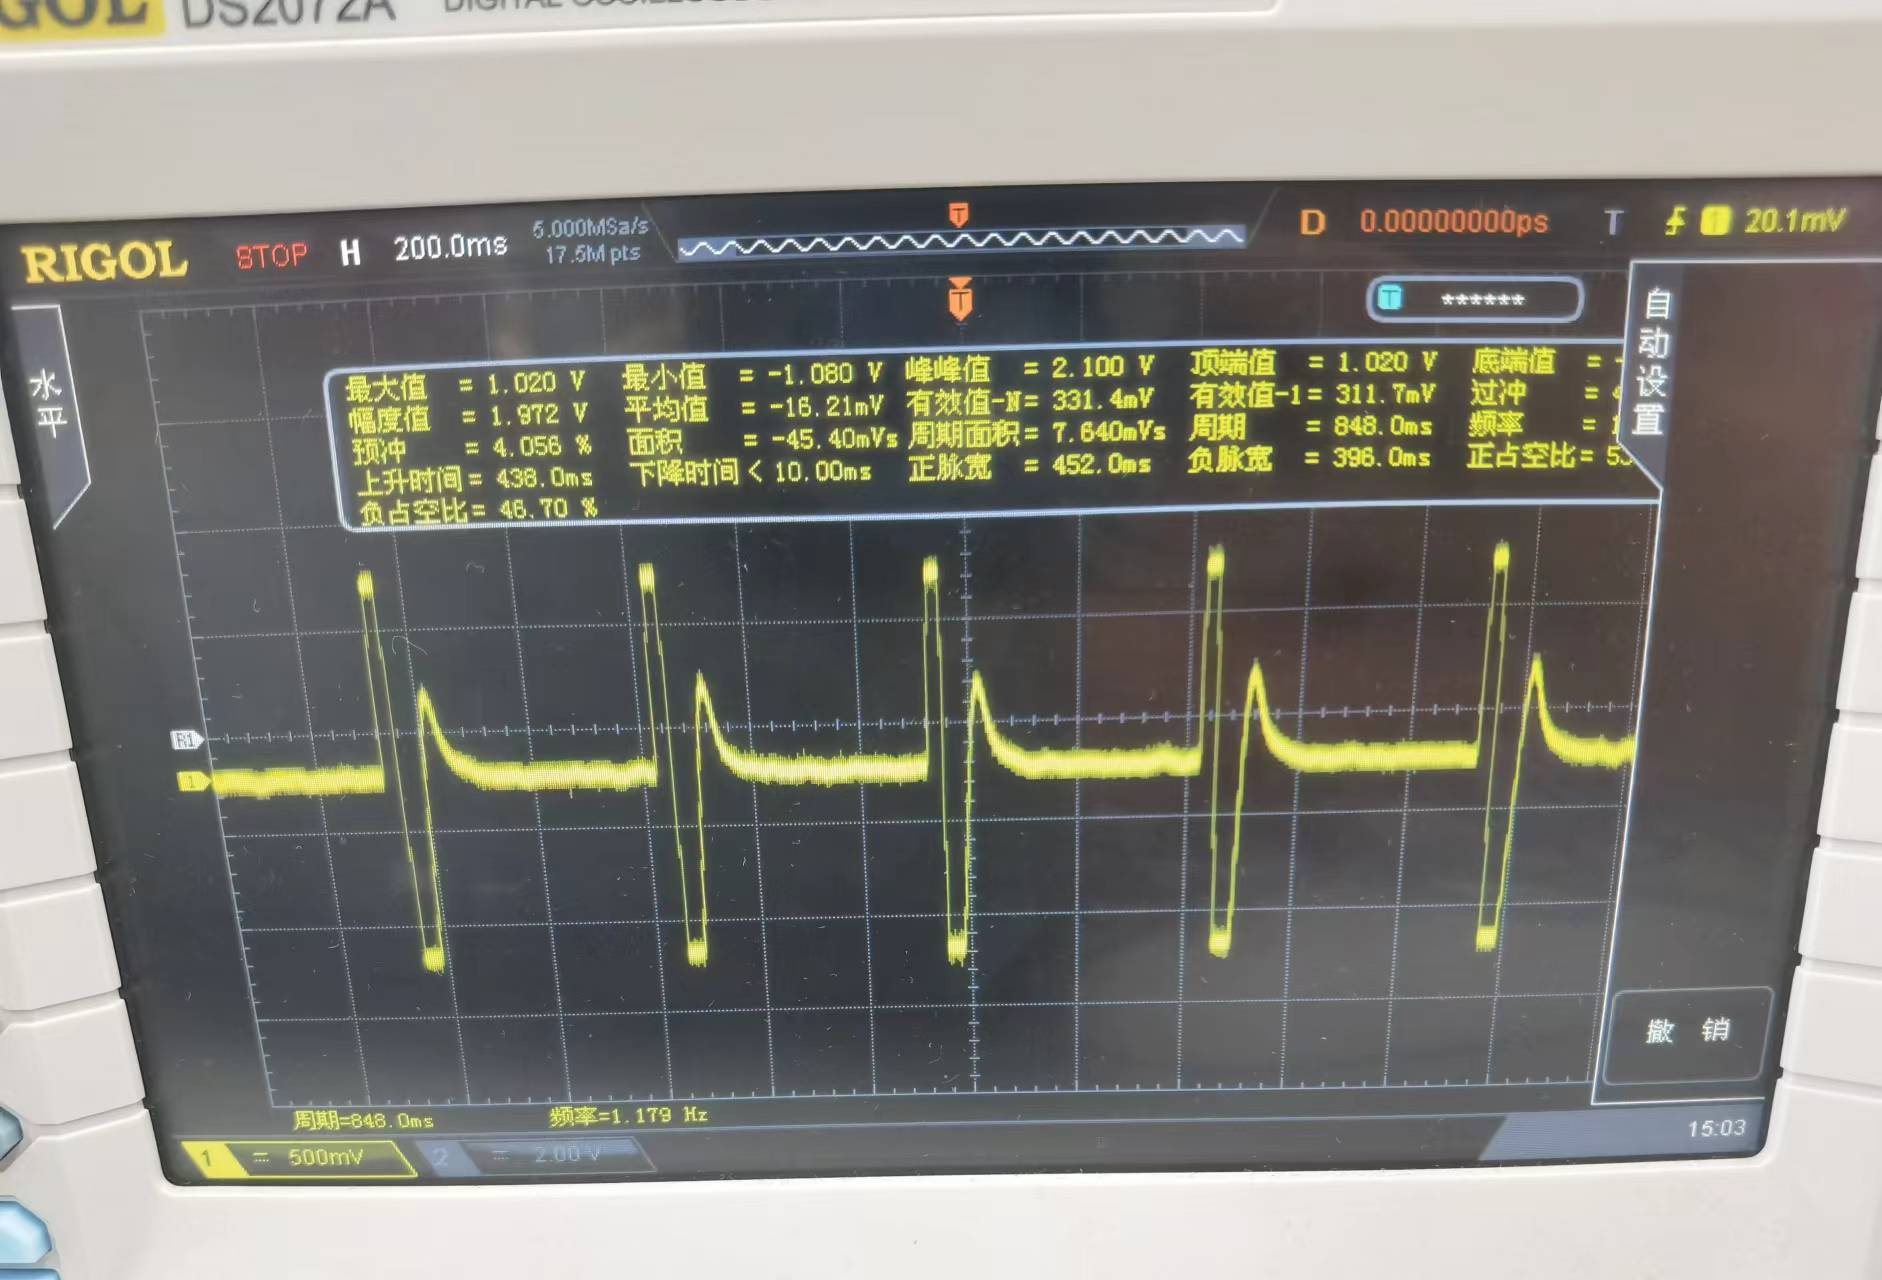
\includegraphics[width=4in]{脉冲波特性}
	\caption{脉冲波特性}%命名并编号
	\label{脉冲波特性}%设置标签
\end{figure}

可以看出,输出的脉冲信号特征明显,并且经差模增益,峰峰值变为了2.1V,说明该系统对脉冲信号的处理效果很好。

\subsubsection{生物电信号波形}

将手指搭到测试点,并增加右脚驱动后,能得到如图所示的生物电信号波形。从图上看,能够看出明显的心电信号,但同时也发现杂波较多,容易干扰心率测量。

\begin{figure}[h]
	\centering%使该部分内容居中
	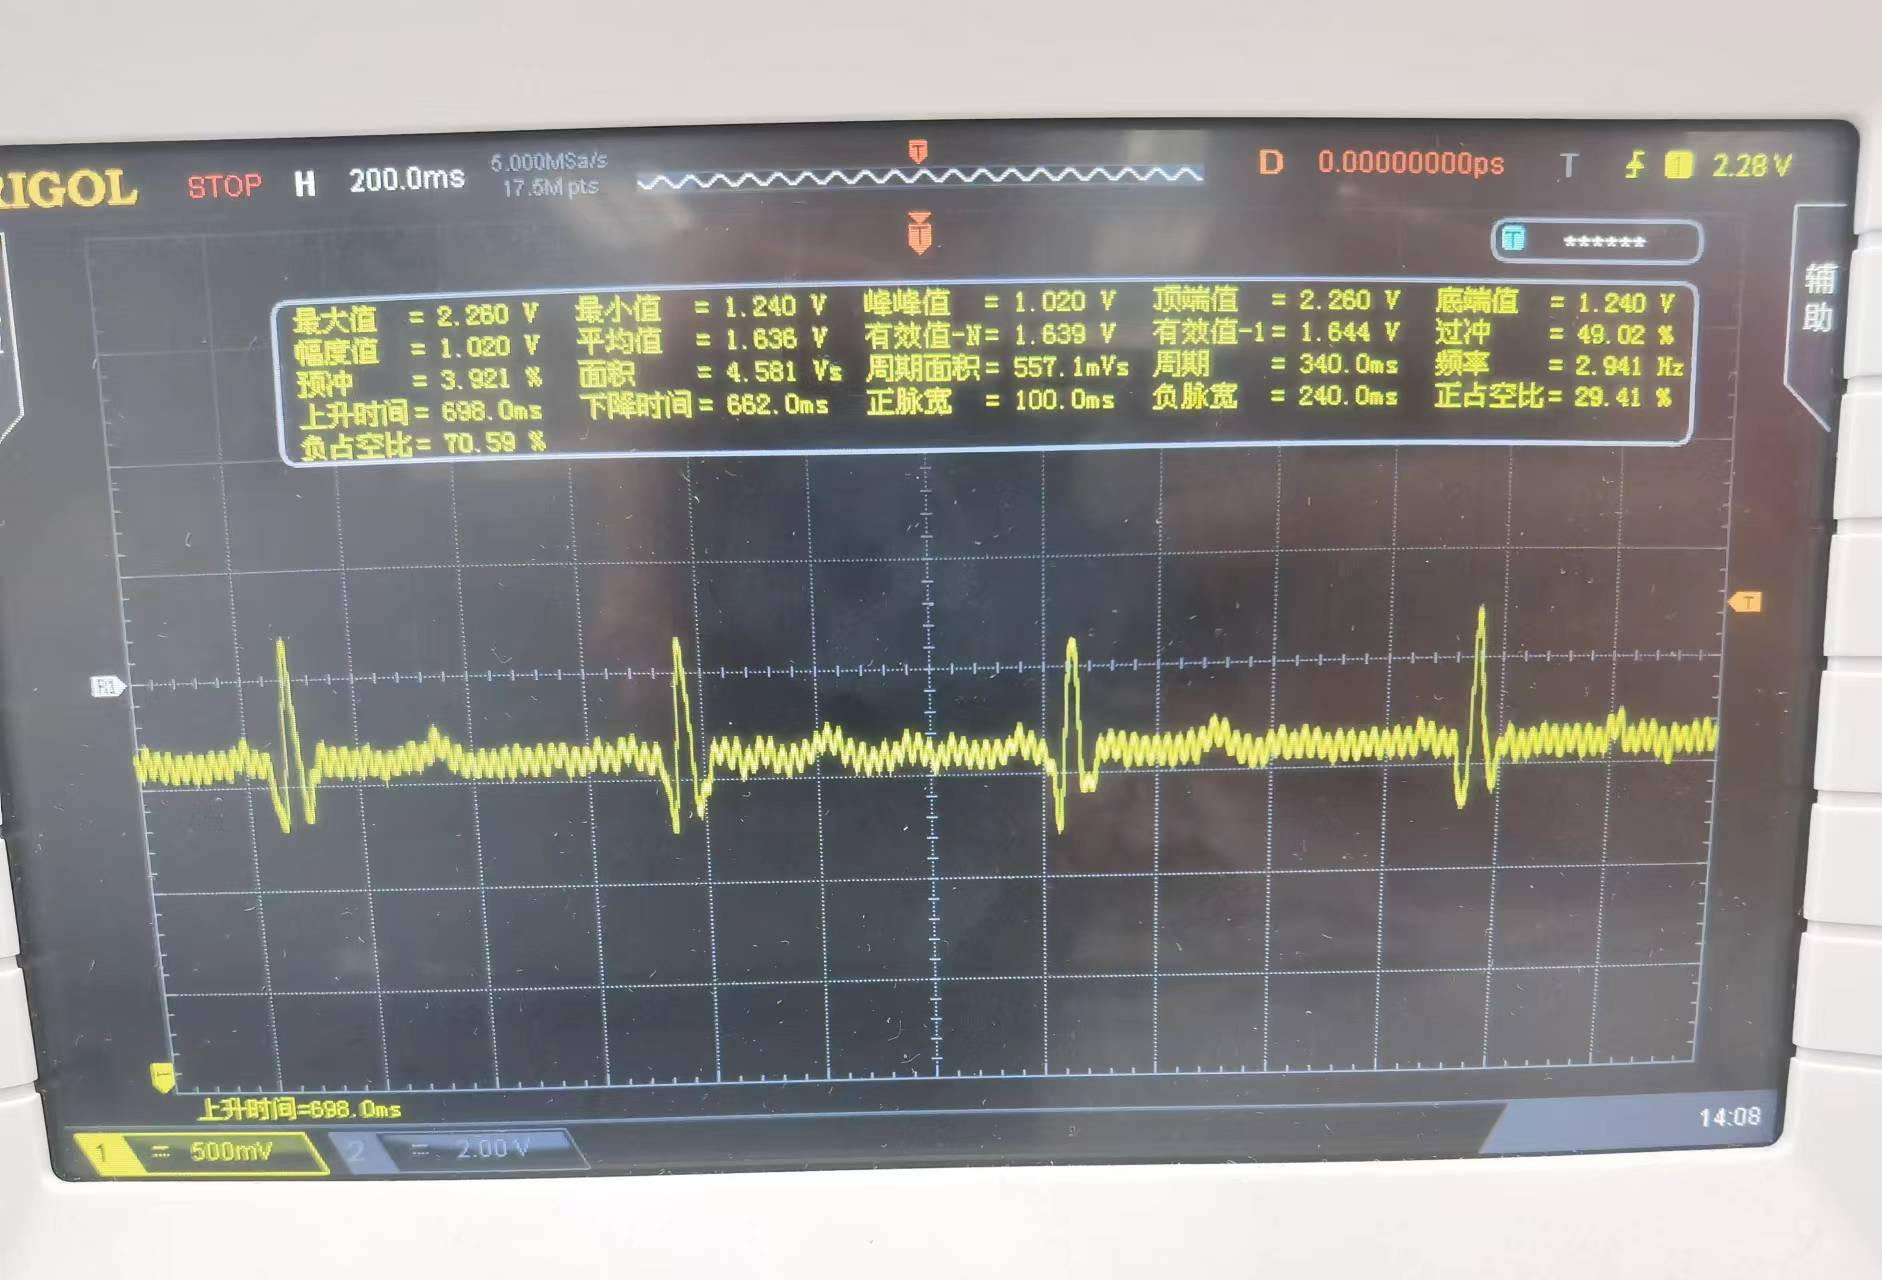
\includegraphics[width=4in]{生物电测试}
	\caption{生物电测试}%命名并编号
	\label{生物电测试}%设置标签
\end{figure}

\subsubsection{螺旋天线制作与测试}

对于工作于一定中心频率的通讯机来说,其所需绕的线
圈数N可以由下式近似算出:

\begin{equation}
	N=\frac{30}{fD}(\frac{L}{D})^(1/5)
\end{equation}
式中,f是工作的中心频率,D是螺旋天线的直径,L是螺旋天线的长度,N是螺旋的圈数。

在实验中,我们选取线径为0.6mm左右,长度为350mm的漆包线,在5mm左右的圆棒上紧密绕制,之后通过矢量网络分析仪测量天线的S11特性曲线。最终我们得到了两个中心频率为436MHz的螺旋天线,如\refeq{天线工作频率}所示。

\begin{figure}[h]
	\centering%使该部分内容居中
	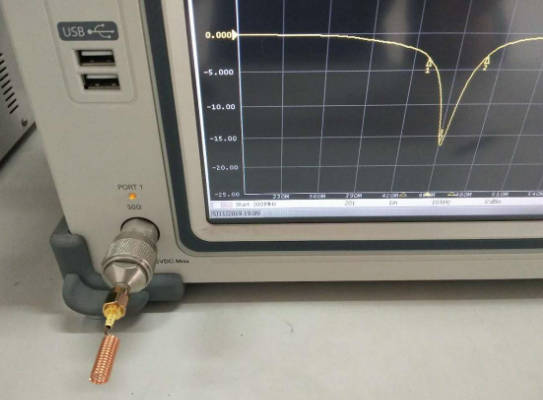
\includegraphics[width=3in]{矢量仪测试结果}
	\caption{天线工作频率}%命名并编号
	\label{天线工作频率}%设置标签
\end{figure}

在后续的测试中,我们用频谱分析仪测试了装载有天线的PCB的工作参数。如图\ref{发射信号功率与工作频率}所示,系统工作在432MHz左右,发射功率为5.02dB,是满足ECG系统设计需求的。

\begin{figure}[h]
	\centering%使该部分内容居中
	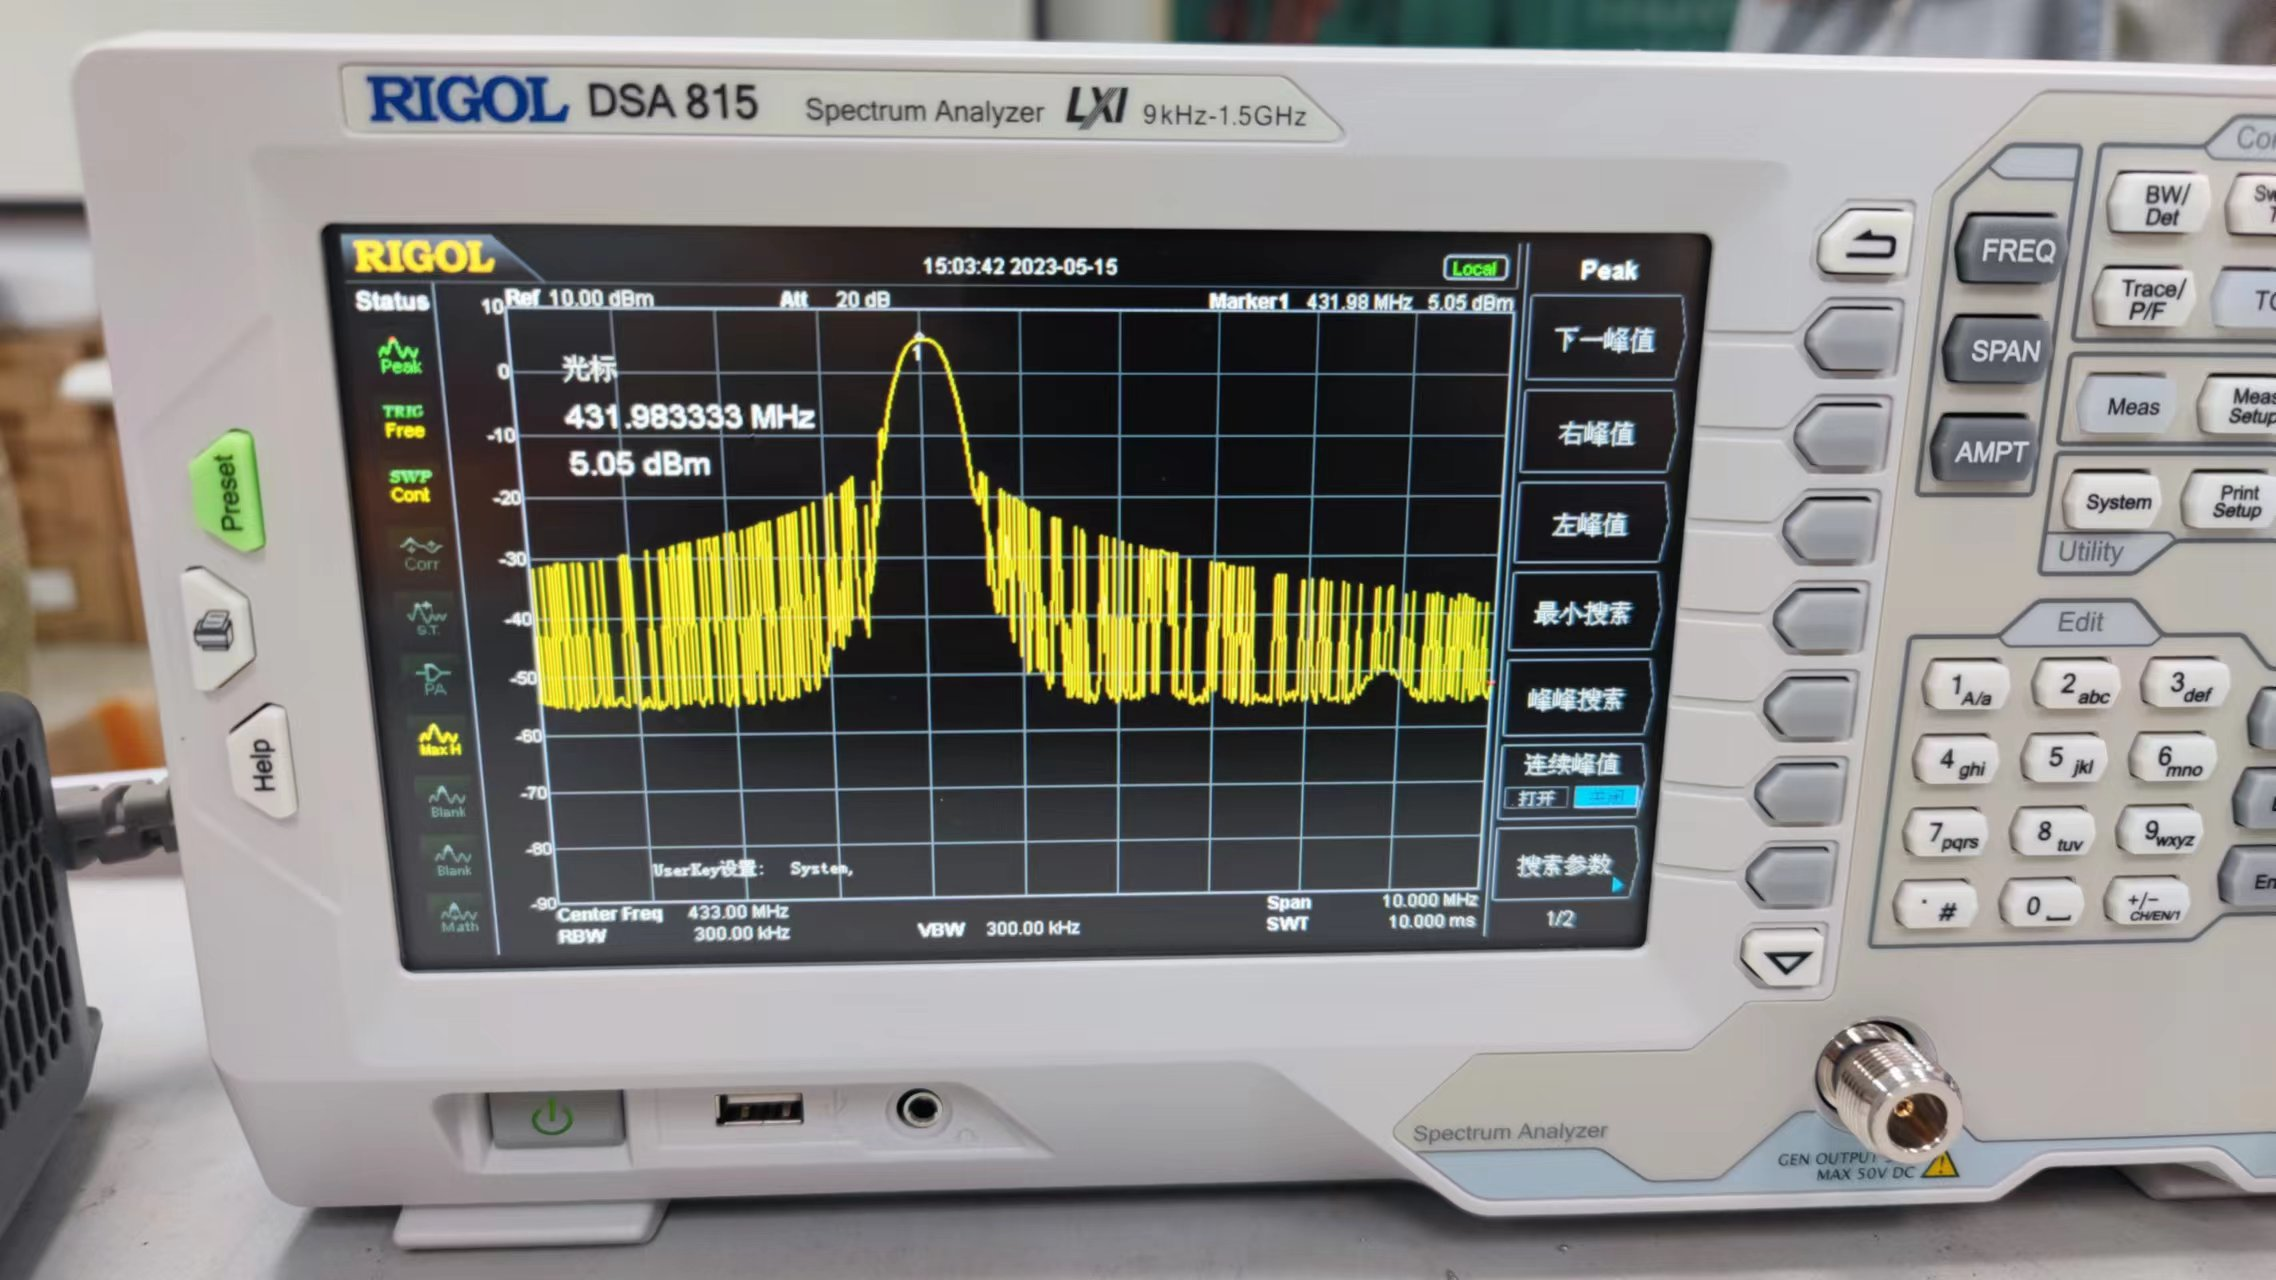
\includegraphics[width=3.5in]{发射信号功率与工作频率}
	\caption{发射信号功率与工作频率}%命名并编号
	\label{发射信号功率与工作频率}%设置标签
\end{figure}

\subsubsection{拉距实验结果分析}

通信距离与系统的发射功率、接收灵敏度和工作频率有以下关系:

\begin{equation}
	[L_{fs}](dB)=32.44+20lg[d(km)]+20lg[f(MHz)]
\end{equation}

式中$L_{fs}$为传输损耗,$d$为传输距离,频率单位为$MHz$。

安装好天线后,将软件发射功率调整到436MHz,利用两台电脑进行拉距实验,最后我们得到的拉距距离为130m,大于设计要求的100m。由于实验时是通过数地砖的方式测量距离,所以测量的数据会有一定的误差。

同时,通过调整射频发送的频率及功率,我们发现:当工作频率降低或发射功率升高时,最终拉距的距离会有增加,这是符合计算理论的。

	
	\subsubsection{硬件电路整体性能分析}
	
	通过之前的各项测试,我们可以大致分析出电路整体的工作性能。
	
	在前端测试部分,系统的共模抑制比符合设计要求,但是共模增益较大,能够得到较为明显的心电信号波形,会导致实际的信号测量时存在一定的杂波,影响心电信号的分析和诊断。
	
	而通过脉冲波测试和实际的生物电测试,可以看出,该系统处理得到峰峰值较大的波形是没有太大问题的,但是在脉冲和脉冲之间的环境噪声也还是较为明显。
	
	最后的发射信号功率测量和拉距实验的实验结果都较为理想,保证了信号在发射端通过射频发射到接受端的过程能够很好地进行。
	
	\subsection{软件设计与调试}
	
	\subsubsection{软件工作流程框图}
	
	\begin{figure}[H]
		\centering%使该部分内容居中
		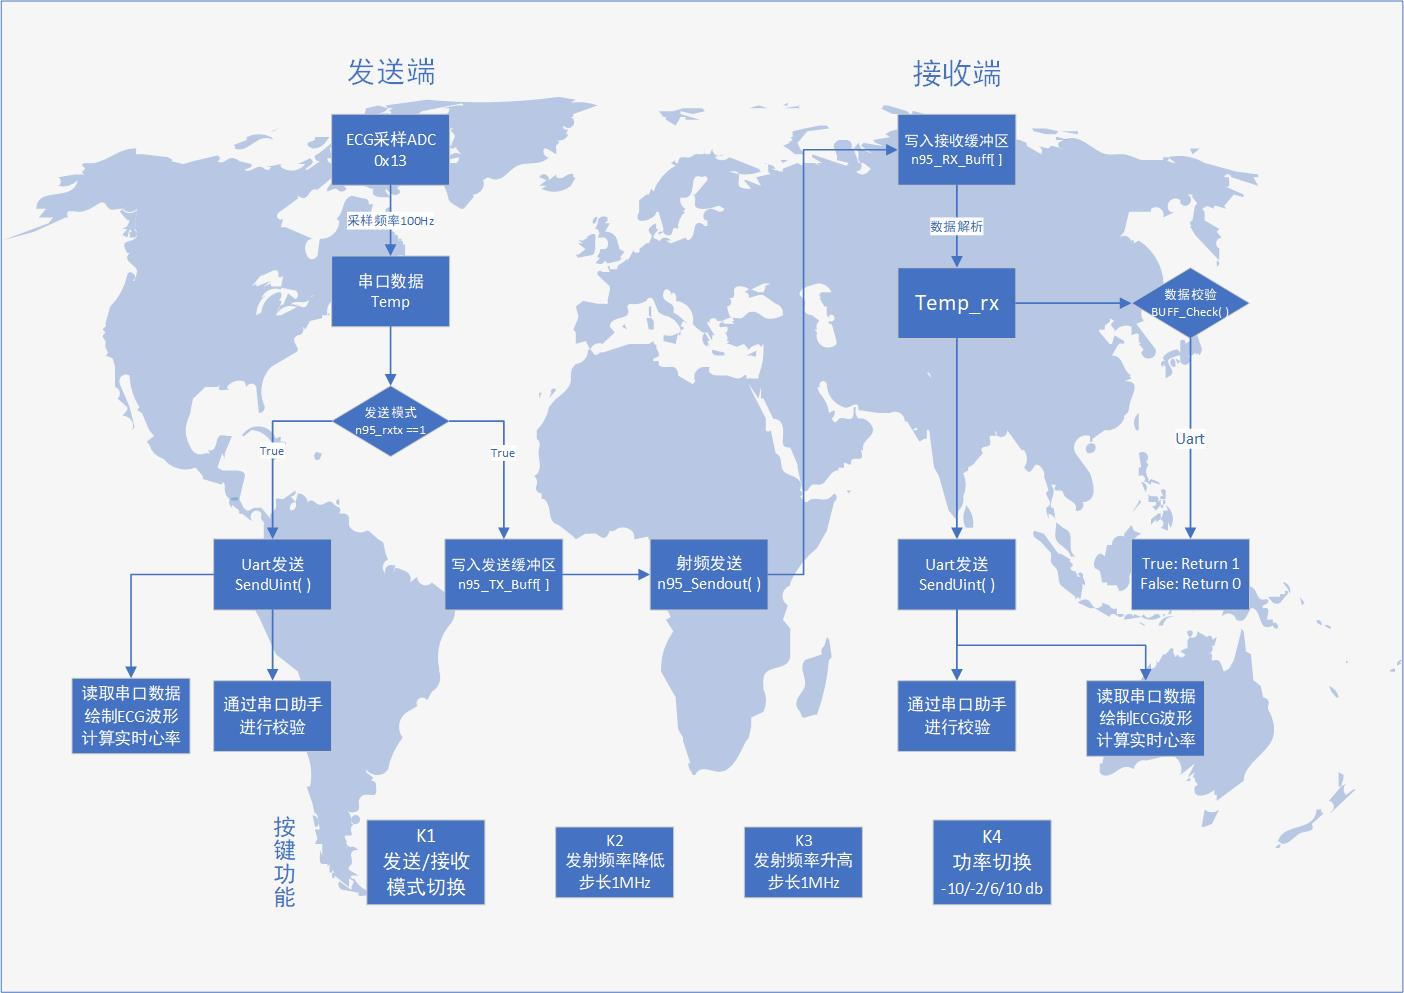
\includegraphics[width=6.5in]{软件工作流程框图}
		\caption{软件工作流程框图}%命名并编号
		\label{软件工作流程框图}%设置标签
	\end{figure}
	
	\subsubsection{软件功能设计}
	
	(1)时序设计  
	    
	    时序设计代码如下,定时器$Timer-Count-1$初始为0,每1ms进1,当其数值达到10之后,开启ECG采样ADC并将定时器归零,从而达到每0.01s进行一次ECG采样(即采样频率为100Hz)
	    
	    \begin{lstlisting}[language=C]
	    	void timer0_int (void) interrupt 1
	    	{
	    		TH0 = 0xfc;
	    		TL0 = 0x18;			//1ms定时中断
	    		
	    		Key_Scan();
	    		//	Run_treat();
	    		++Timer_Count_1;
	    		
	    		if (Timer_Count_1 > 9)  //0.01s开启ECG的采样
	    		{
	    			timer_flag_ECG = 1;
	    			Timer_Count_1 = 0;
	    		}
	    	}
	    \end{lstlisting}
	  
	   ~\\
	    
	(2)AD功能                   
	        
	        ADC初始设置代码如下 
	         \begin{lstlisting}[language=C]
	         	void ADC0_Init_ECG (void) //ECG_ADC
	         	{
	         		ADC0CN = 0x00;                      // ADC0 disabled, normal tracking, 
	         		// conversion triggered on "ADC0BUSY" set
	         		REF0CN = 0x08;                      // disable on-chip VREF and buffer
	         		AMX0P = 0x13;      //ECG传感器开启  // ADC0 positive input = P1.1 
	         		AMX0N = 0x1F;                       // ADC0 negative input = GND
	         		
	         		ADC0CF = ((SYSCLK/3000000)-1)<<3;   // set SAR clock to 3MHz
	         		ADC0CF &= ~0x04;                    // right-justify results 
	         		EIE1 |= 0x08;              // enable ADC0 conversion complete int.
	         		AD0EN = 1;                          // enable ADC0
	         	}
	         \end{lstlisting}
	         
	         读取串口数值并作AD转换处理的代码如下
	          \begin{lstlisting}[language=C]
	         	void ADC0_ISR (void) interrupt 10
	         	{
	         		unsigned long result=0;
	         		// unsigned long mV;                         // Measured voltage in mV
	         		AD0INT = 0;                     // Clear ADC0 conv. complete flag
	         		result = ADC0;
	         		Temp =  result * 3300 / 1023;   
	         		//   printf("P1.1 voltage: %ld mV\n",mV);
	         \end{lstlisting}
	    
	     ~\\
	              
	(3)串口功能  
	            
	       通过Uart发送int型数据/char型数据/字符串数据的代码如下
	       \begin{lstlisting}[language=C]
	       	void SendUint(uint Data)
	       	{
	       		Uart_Send_Buff[0] = (Data / 1000 % 10) +0x30;
	       		Uart_Send_Buff[1] = (Data / 100 % 10) +0x30;
	       		Uart_Send_Buff[2] = (Data / 10 % 10) +0x30;
	       		Uart_Send_Buff[3] = (Data %10) +0x30;
	       		//	Uart1_tx_len = 4;
	       		for (Uart_Send_Count=0;Uart_Send_Count<4;Uart_Send_Count++)
	       		{
	       			SBUF0 = Uart_Send_Buff[Uart_Send_Count];
	       			while(TI0 ==0){}
	       			TI0 = 0;
	       		}
	       	}
	       	\end{lstlisting}
	       
	       \begin{lstlisting}[language=C]
	       	void SendUchar(char Data)
	       	{
	       		Uart_Send_Buff[0] = (Data / 10 % 10) +0x30;
	       		Uart_Send_Buff[1] = (Data %10) +0x30;
	       		//	Uart1_tx_len = 2;
	       		for (Uart_Send_Count=0;Uart_Send_Count<2;Uart_Send_Count++)
	       		{
	       			SBUF0 = Uart_Send_Buff[Uart_Send_Count];
	       			while(TI0 ==0){}
	       			TI0 = 0;
	       		}
	       	}
	       \end{lstlisting}
	       
	        \begin{lstlisting}[language=C]
	       	void SendString(char *s)
	       	{
	       		uchar	i=0;
	       		while (*s)
	       		{
	       			Uart_Send_Buff[i++] = *s++;
	       		}
	       		//Uart1_tx_len = i;
	       		for (Uart_Send_Count=0;Uart_Send_Count<i;Uart_Send_Count++)
	       		{
	       			SBUF0 = Uart_Send_Buff[Uart_Send_Count];
	       			while(TI0 ==0){}
	       			TI0 = 0;
	       		}
	       	}
	       \end{lstlisting}
	       
	       在$main$函数中,我们将ADC输出的数值$Temp$通过$void \quad SendUint(uint \quad Data)$函数发送,并配合字符串函数发送指定格式,我们就能在串口中读取到相应的数值。
	          
	         \newpage
	          	               
	(4)nRF905功能   
	
	nRF905初始化函数入下,通过该函数可以将其转换为接收模式
	\begin{lstlisting}[language=C]
	void n95_Init_Dev(uchar band,uint freq,uchar pwr)
	{
		uchar i = 0;
		
		nPin_PWR_UP = 1;									// PWR_UP置高,nRF905进入上电模式	
		nPin_TRX_CE = 0;									// TRX_CE置低,进入待机和SPI操作模式
		nPin_CSN = 0;										// CSN置低,   进入SPI操作模式
		SPI_Byte_Write_Read(nCMD_W_CONFIG);					// 向nRF905发送"写配置寄存器命令"
		SPI_Byte_Write_Read(freq & 0xFF);					// RF通道bit7:0
		SPI_Byte_Write_Read(nRCD_AUTO_RETRAN_disanble		// 禁用自动重发 
		| nRCD_RX_RED_PWR_disanble			// 禁用低功耗RX模式
		| (pwr<<2)							// 输出功率为10dBm
		| (band<<1)							// 工作频段设置
		| (freq>>8) );						// RF通道bit8
		SPI_Byte_Write_Read(nRCD_TX_AFW_4byte				// TX地址宽度为4byte
		| nRCD_RX_AFW_4byte);					// RX地址宽度为4byte
		SPI_Byte_Write_Read(RF_DATA_WIDTH);					// RX数据宽度
		SPI_Byte_Write_Read(RF_DATA_WIDTH);					// TX数据宽度
		
		for(i=0; i<4; i++){
			SPI_Byte_Write_Read(n95_RF_Addr[i]);			// RX地址 byte0~3
		}
		
		SPI_Byte_Write_Read(nRCD_CRC_MODE_16crc				// 16bitCRC
		| nRCD_CRC_EN_enable					// 启用CRC
		|	nRCD_XOF_16MHz						// 外部晶振频率为16MHz
		|	nRCD_UP_CLK_EN_disanble				// 禁用外部时钟输出
		| nRCD_UP_CLK_FREQ_4MHz);				// 时钟输出为4MHz
		
		nPin_CSN = 1;										// CSN置高,   退出SPI操作模式
		nPin_TX_EN = 0;										// TX_EN置低 ,进入接收模式
		nPin_TRX_CE = 1;									// TRX_CE置高,进入工作模式
	}      
\end{lstlisting}   
	   
	   下面的代码将发送端缓冲区n95-TX-Buffer的数据通过nRF905发送到接收端,调试过程中我们发现最后两行代码中等待进入接收模式的时间过长,严重影响到了串口的数据发送频率,因此我们将这两句省去并在完成优化之后添加在$main$函数中。
	   \begin{lstlisting}[language=C]
	   void n95_Sendout(uchar *p)
	   {
	   	uchar i=0;
	   	nPin_PWR_UP = 1;							// PWR_UP置高,nRF905进入上电模式
	   	nPin_TRX_CE = 0;							// TRX_CE置低,进入待机和SPI操作模式
	   	nPin_TX_EN = 1;								// TX_EN置高 ,进入发送模式
	   	
	   	nPin_CSN = 0;								// CSN置低,   进入SPI操作模式
	   	SPI_Byte_Write_Read(nCMD_W_TX_ADDRESS);		// 向nRF905写入"写TX地址"指令
	   	for(i=0; i<4; i++){
	   		SPI_Byte_Write_Read(n95_RF_Addr[i]);	// 写入TX地址 byte0~3,注意此处应与"nRCD_TX_AFW"的配置一致
	   	}
	   	nPin_CSN = 1;								// CSN置高,   退出SPI操作模式
	   	Delay(1);
	   	nPin_CSN = 0;								// CSN置低,   进入SPI操作模式
	   	SPI_Byte_Write_Read(nCMD_W_TX_PAYLOAD);		// 向nRF905写入"写TX数据"指令
	   	for(i=0; i<RF_DATA_WIDTH; i++){
	   		SPI_Byte_Write_Read(p[i]);				// 写入待发送数据
	   	}
	   	nPin_CSN = 1;								// CSN置高,   退出SPI操作模式
	   	
	   	nPin_TRX_CE = 1;							// TRX_CE置高,进入发送模式
	   	//while(nPin_DR == 0);						// 等待DR置高,发送完成
	   	//nPin_TX_EN = 0;								// TX_EN置低 ,进入接收模式
	   }
	\end{lstlisting} 
	   
	   下面的代码用于检查nRF905是否接收到数据,如接收到数据将数据存入接收缓冲区,并返回成功标志。
	   \begin{lstlisting}[language=C]
	   	uchar n95_Check_DR(uchar *p)
	   	{	uchar i=0;
	   		
	   		if(nPin_DR == 1){
	   			nPin_TRX_CE = 0;						// TRX_CE置低,进入待机模式
	   			nPin_CSN = 0;							// CSN置低,   进入SPI操作模式
	   			
	   			SPI_Byte_Write_Read(nCMD_R_RX_PAYLOAD);	// 向nRF905写入"读取RXFIFO"指令
	   			
	   			for(i=0; i<RF_DATA_WIDTH; i++){
	   				p[i] = 	SPI_Byte_Write_Read(0);		// 读取接收数据
	   			}
	   			
	   			nPin_CSN = 1;							// CSN置高,   退出SPI操作模式
	   			nPin_TRX_CE = 1;						// TRX_CE置高,进入工作模式
	   			return(1);								// 返回接收成功标志
	   		}else{
	   			return(0);								// 返回未接收到数据标志
	   		}
	   	}
	   \end{lstlisting} 
	   
	   在$main$函数中,我们将ADC读取的数值存入发送缓冲区并发送,同时在接收端进行数据解析,将接收缓冲区的数组转换为int型数据,如下。
	   
	    \begin{lstlisting}[language=C]
	   // 发送端
	   //取数字部分(只传输数值部分,便于接收部分重新读取)
	   n95_TX_Buff[index] = Temp/1000+0x30;//取千位
	   index++;
	   n95_TX_Buff[index] = (Temp/100%10)+0x30;//取百位
	   index++;
	   n95_TX_Buff[index] = (Temp/10%10)+0x30;//取十位
	   index++;
	   n95_TX_Buff[index] = (Temp %10)+0x30;//取个位
	   index++;
	   //发送nRF905缓冲区的数据
	   n95_Sendout(n95_TX_Buff);
	   memset(n95_TX_Buff, 0, RF_DATA_WIDTH);
	   
	   // 接收端
	   if(n95_RX_Buff[0]!=NULL){  //表示接收到对应的信号
	   	Temp_rx+=(n95_RX_Buff[index]-0x30)*1000;//取千位
	   	index++;
	   	Temp_rx+=(n95_RX_Buff[index]-0x30)*100;//取百位
	   	index++;
	   	Temp_rx+=(n95_RX_Buff[index]-0x30)*10 ;//取十位
	   	index++;
	   	Temp_rx+=(n95_RX_Buff[index]-0x30);//取个位
	   	index++;
	   	}
	   
	   
	   \end{lstlisting} 
	   
	   
	    ~\\
	             
	(5)按键功能
	
	按键扫描函数如下,通过检测下降沿触发来判断按键是否按下
	\begin{lstlisting}[language=C]
		void	Key_Scan()
		{
			P4_IN = P4;
			
			if (!Key1)			//键扫描1,检测下降沿
			{
				if(Key1_back)
				{
					Key1_press_flag = 1;
				}
			}
			
			if (!Key2)			//键扫描2
			{
				if(Key2_back)
				{
					Key2_press_flag = 1;
				}
			}
			
			if (!Key3)			//键扫描3
			{
				if(Key3_back)
				{
					Key3_press_flag = 1;
				}
			}
			
			if (!Key4)			//键扫描4
			{
				if(Key4_back)
				{
					Key4_press_flag = 1;
				}
			}
			
			Key1_back = Key1;
			Key2_back = Key2;
			Key3_back = Key3;
			Key4_back = Key4;
		}
	\end{lstlisting} 
	
	按键K1至K4的功能设计函数如下,其中K1用于调整收发模式,K2用于降低系统工作频率(步长为1MHz),K3用于提高系统工作频率,K4用于调整射频发送功率
	
	\begin{lstlisting}[language=C]
		// 收发模式控制,LED点亮时处于发送模式
		if (Key1_press_flag)
		{
			Key1_press_flag = 0;
			n95_rxtx++;
			n95_rxtx &= 0x01;
			if (n95_rxtx)
			{
				LED1_ON;//LED1亮表示发送模式
			}
			else
			{
				LED1_OFF;
				//LED1暗表示接收模式
			}
			n95_Init_Dev(n95_band, n95_freq, n95_pwr);
			UartSend_RF_Set();
		}
	\end{lstlisting} 
	
	\begin{lstlisting}[language=C]
		//频率递减,步距是1MHz,频率范围是423-472Mhz,起始频率为436MHz
		if (Key2_press_flag)
		{
			LED2_ON;
			Delay(100);
			LED2_OFF;
			Key2_press_flag = 0;
			if (n95_freq >= 40) {n95_freq -= 10;} //每次改变1MHz,最小频率是423MHz
			n95_Init_Dev(n95_band, n95_freq, n95_pwr);
			UartSend_RF_Set();
		}
	\end{lstlisting} 
	
	\begin{lstlisting}[language=C]
		//频率递增
		if (Key3_press_flag)
		{
			LED3_ON;
			Delay(100);
			LED3_OFF;
			Key3_press_flag = 0;
			if (n95_freq <=510 ) {n95_freq += 10;}//每次改变1MHz,最大频率是472MHz 
			n95_Init_Dev(n95_band, n95_freq, n95_pwr);
			UartSend_RF_Set();
		}
	\end{lstlisting} 
	
	\begin{lstlisting}[language=C]
		//功率调整
		if (Key4_press_flag)
		{
			LED4_ON;
			Delay(100);
			LED4_OFF;
			Key4_press_flag = 0;
			n95_pwr++;
			n95_pwr &= 0x03;
			n95_Init_Dev(n95_band, n95_freq, n95_pwr);
			UartSend_RF_Set();
		}
	\end{lstlisting} 
	
	\newpage
	
	(6)射频工作频率及发射功率显示
	
	当我们通过按键调整nRF905的工作频率及发射功率时,可以通过此函数将目前的工作参数打印至串口,方便我们进行调试。
	
	\begin{lstlisting}[language=C]
		void UartSend_RF_Set(void)
		{
			uint freq=0;
			uchar pwr=0;
			
			SendString("RF905, Freq: ");
			freq = (4200 + n95_freq) * (1 + n95_band);//n95_freq=4320-4200
			SendUint(freq/10);
			SendString(".");
			SendUchar((freq%10)*10);
			SendString("MHz,");
			
			if(n95_rxtx ==0){
				SendString(" Mod: R ,");}
			else	{
				SendString(" Mod: T ,");}
			
			// 发射功率转换
			switch(n95_pwr){
				case 0:{	// -10
					SendString("Power:-10dBm\n");
				}break;
				case 1:{	// -2
					SendString("Power: -2dBm\n");
				}break;
				case 2:{	// 6
					SendString("Power:  6dBm\n");
				}break;
				case 3:{	// 10
					SendString("Power: 10dBm\n");
				}break;
			}
			
		}
	\end{lstlisting} 

	~\\
	
	(6)波形自动绘制及心率实时测量
	
	我们通过$MATLAB$编程制作了一个可以用于自动绘制波形及测量心率的小程序,如图\ref{APP窗口}。该程序可以通过读取串口数值进行实时绘图与计算心率,同时,当心率过高或过低时(大于120、小于40)下方LED会变红进行警告。
	
	\begin{figure}[H]
		\centering%使该部分内容居中
		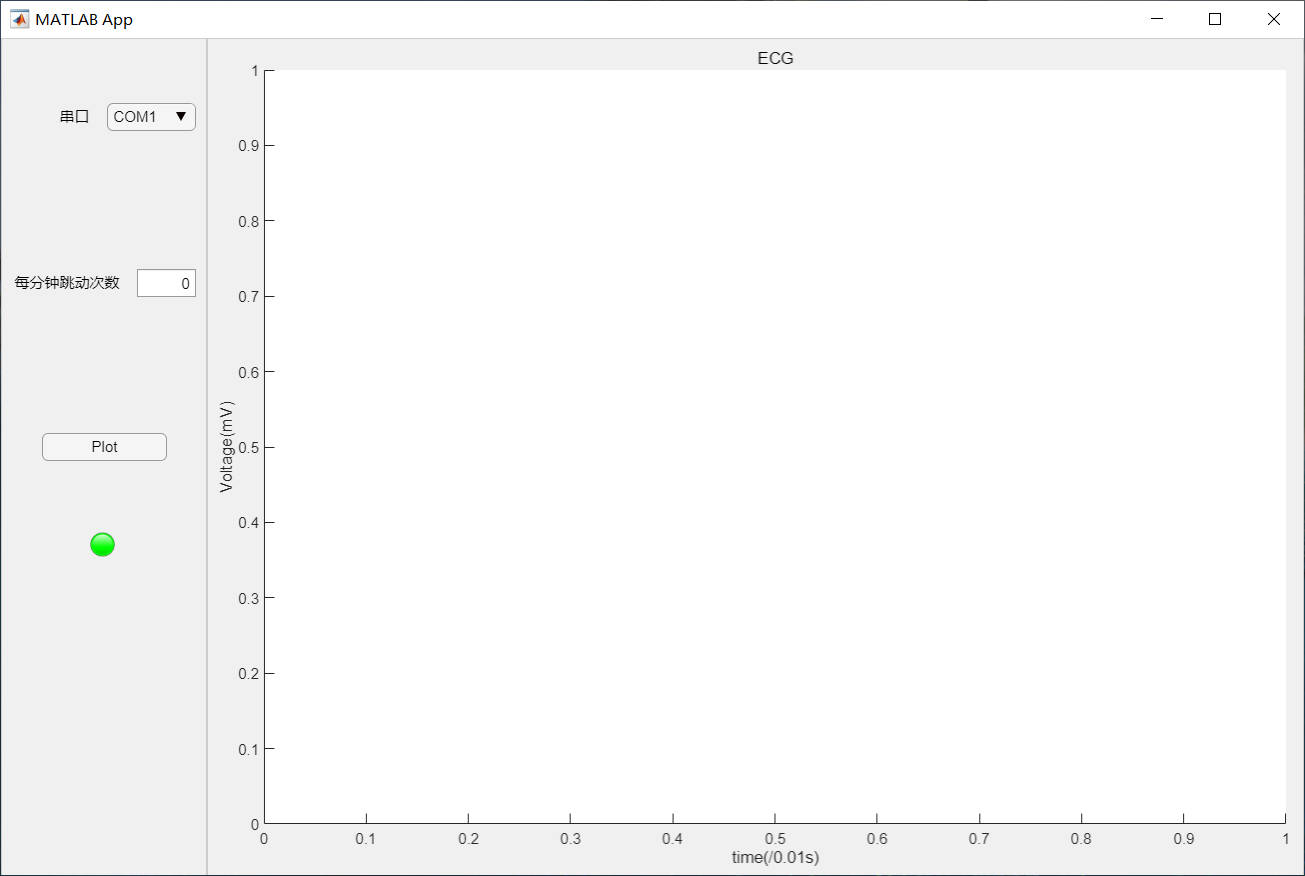
\includegraphics[width=5in]{APP窗口}
		\caption{APP窗口}%命名并编号
		\label{APP窗口}%设置标签
	\end{figure}

\begin{figure}[H]
	\centering%使该部分内容居中
	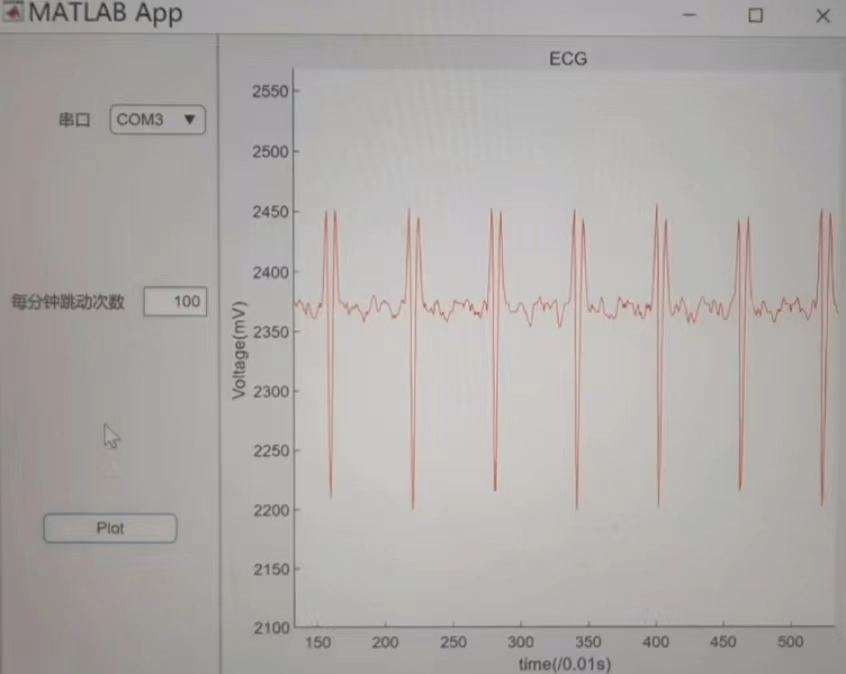
\includegraphics[width=5in]{APP工作演示}
	\caption{APP工作演示}%命名并编号
	\label{APP工作演示}%设置标签
\end{figure}
	
	\newpage
	
	相应代码如下
	\begin{lstlisting}[language=Matlab]
		s=serialport(app.DropDown.Value,115200);
		flush(s);
		configureTerminator(s,"CR");
		
		InputBufferSize = 400;
		margin = 100;
		t = 1:InputBufferSize;
		InputBuffer = zeros(1,InputBufferSize);
		
		for i=1:4000
		while InputBuffer(1)==0
		for n = 2:InputBufferSize
		InputBuffer(n-1) = InputBuffer(n);
		end
		out = readline(s); 
		InputBuffer(InputBufferSize) = out;
		end
		
		t=t+1;
		
		for j = 2:InputBufferSize
		InputBuffer(j-1) = InputBuffer(j);
		end
		out = readline(s); 
		InputBuffer(InputBufferSize) = out;
		plot(app.UIAxes,t,InputBuffer(1,:),'-r');
		axis(app.UIAxes,[t(1) t(InputBufferSize) min(InputBuffer)-margin max(InputBuffer)+margin+10]);
		pause(0.1);
		
		[m,im]=min(InputBuffer(1:200));
		for k=im+10:InputBufferSize
		if(abs(InputBuffer(k)-m)<=50)
		imm=k;
		break;
		else
		imm=im;
		end
		end
		
		T=0.01*(imm-im);
		
		q=60/T;
		
		if(q>=120 || q<=40)
		app.Lamp.Color="1,0,0";
		else
		app.Lamp.Color="0,1,0";
		end
		
		app.EditField.Value=q;
		
		%print(T);
		end
	\end{lstlisting} 
	
	\subsubsection{软件调试}
	
	(1)调试环境和方法
	
	本次实验中我们采用Keil作为开发环境,同时配合Debugger进行程序的定点调试与烧录。
	
	\begin{figure}[H]
		\centering%使该部分内容居中
		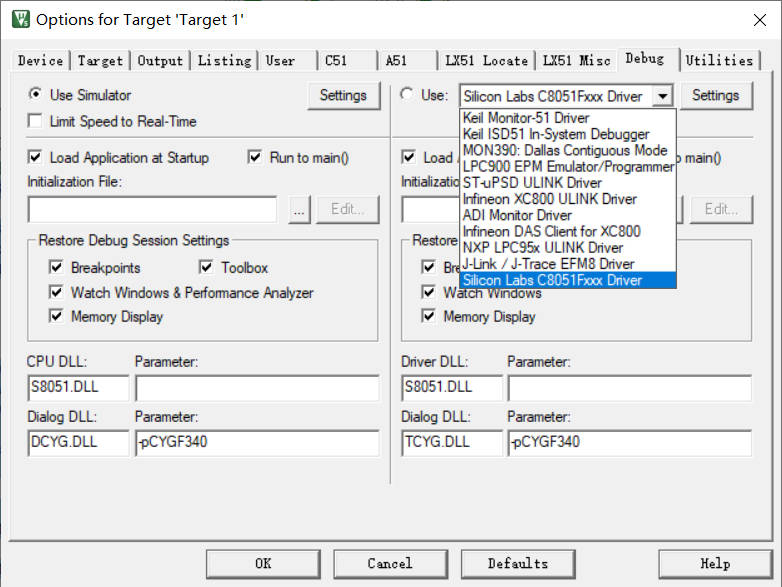
\includegraphics[width=3.5in]{调试环境}
		\caption{调试环境}%命名并编号
	\end{figure}
	
	\newpage
	
	(2)波形采样,串口显示   
	              
	 在调试过程中,我们将模拟ECG信号接发送端的输入,可以通过接收端的串口显示数据,并利用心电GUI显示软件观察采样波形,如下图
	 
	 \begin{figure}[H]
	 	\centering
	 	\begin{minipage}[t]{0.49\linewidth}%%%%%%%%%note2
	 		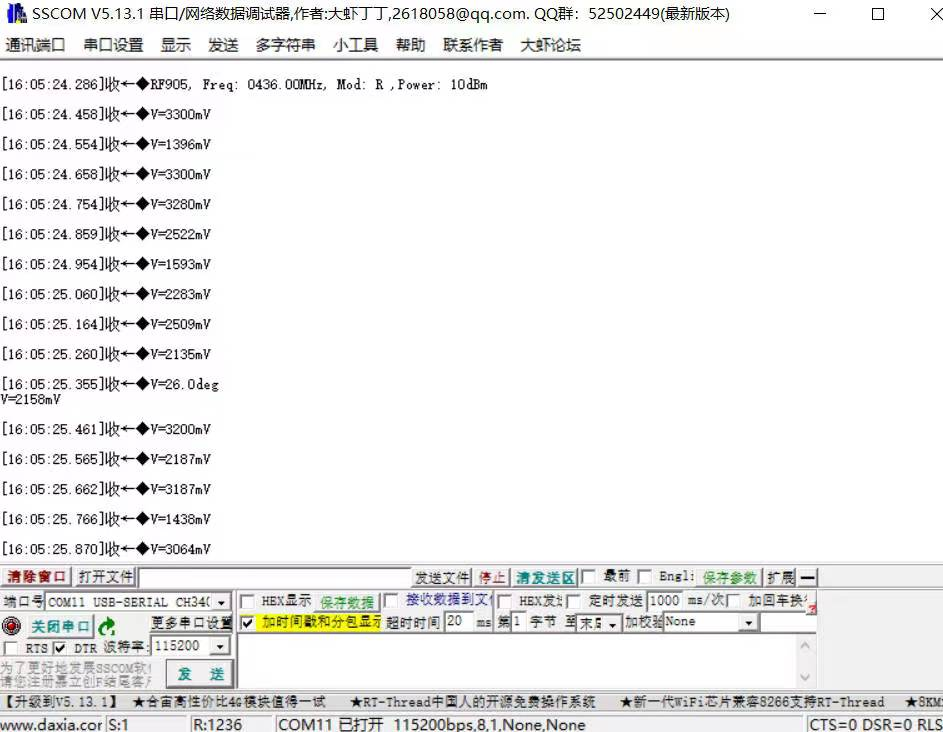
\includegraphics[width=0.9\linewidth]{串口显示}%%%%%%%%%note3
	 		\caption{串口显示}
	 	\end{minipage}%
	 	\begin{minipage}[t]{0.49\linewidth}
	 		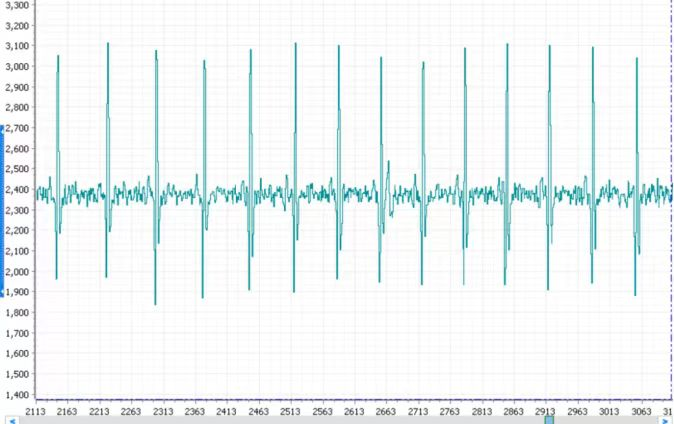
\includegraphics[width=0.9\linewidth]{波形采样}
	 		\caption{采样波形}
	 	\end{minipage}
	 \end{figure}           
	              
	               
	(3)模块之间数据通讯      
	
	在调试过程中,我们将发送格式设置为“Send an ECG signal:xxx”,接收格式设为“Receive an ECG signal:xxx”,下图为一次调试过程中的串口显示结果,可以看出发送与接收模块之间的数据通讯是精确且迅速的。
	
	\begin{figure}[H]
		\centering
		\begin{minipage}[t]{0.49\linewidth}%%%%%%%%%note2
			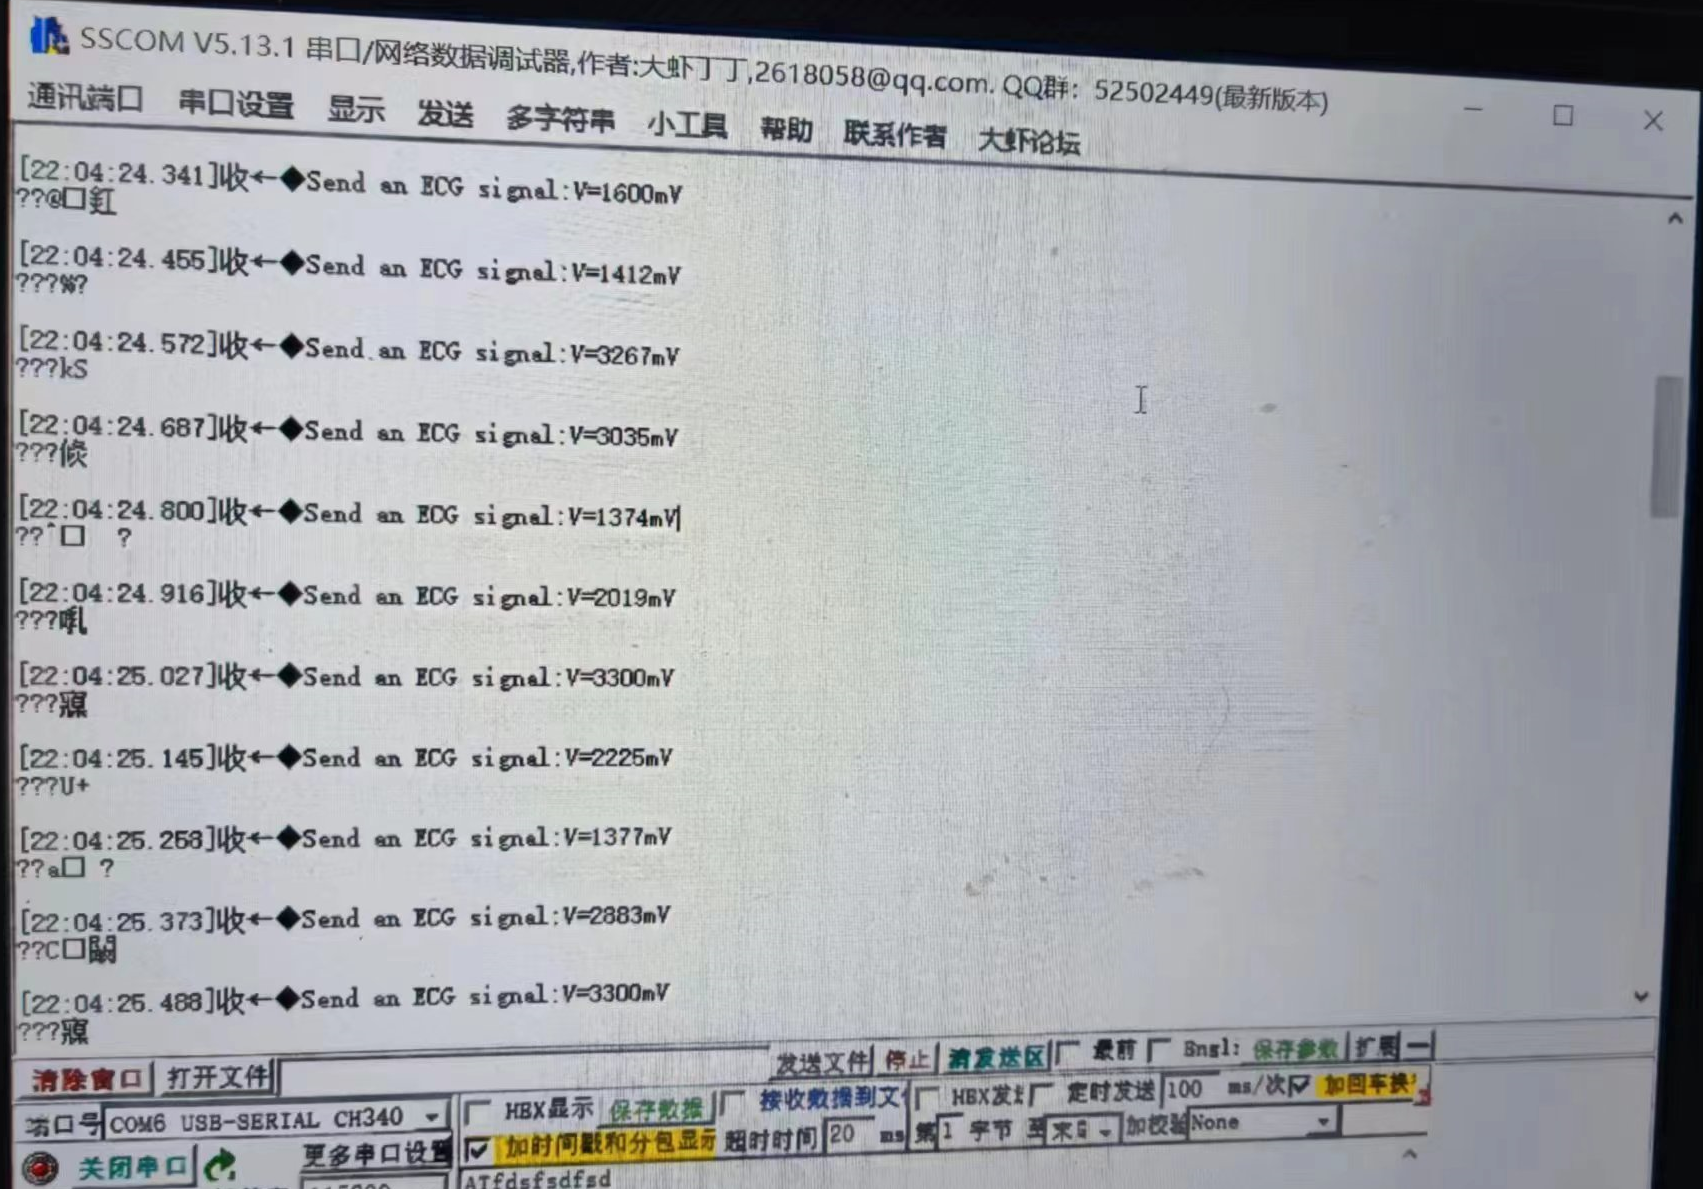
\includegraphics[width=0.9\linewidth]{发送端串口显示}%%%%%%%%%note3
			\caption{发送端串口显示}
		\end{minipage}%
		\begin{minipage}[t]{0.49\linewidth}
			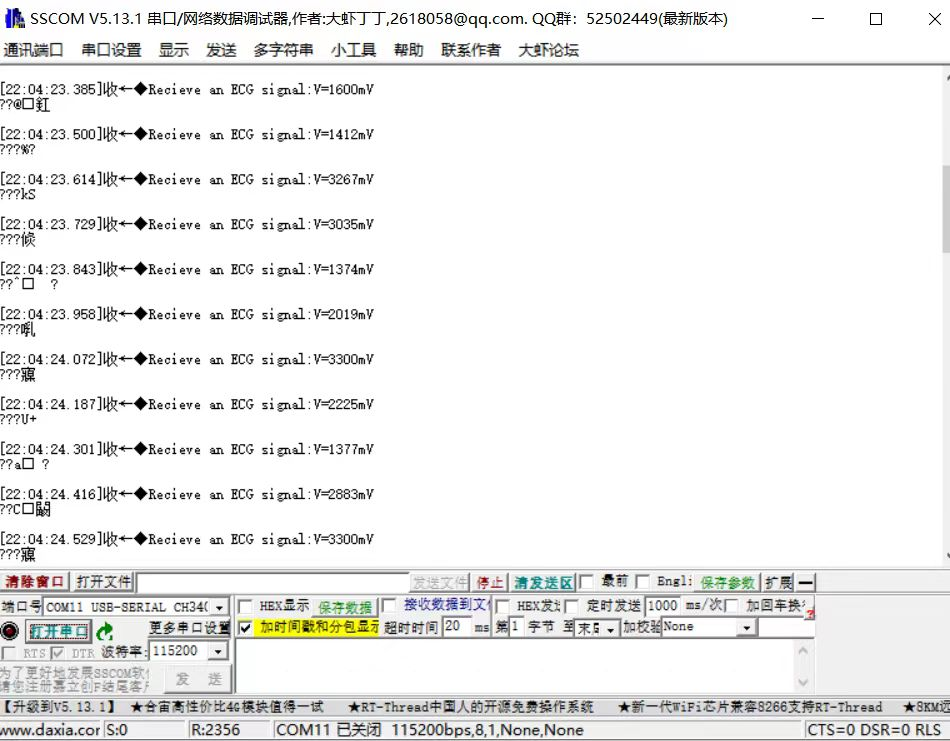
\includegraphics[width=0.9\linewidth]{接收端串口显示}
			\caption{接收端串口显示}
		\end{minipage}
	\end{figure}
	
	\newpage
	
	\section{总结}
	
	\subsection{系统装调过程中遇到的问题和解决情况}
	
	\subsubsection{采样频率与串口接收频率不匹配}
	
	在调试过程中,我们发现设置采样频率为100Hz后,串口端接收数据的频率依然保持10Hz不变。通过检查,我们发现是main函数中出现有delay(100)函数,每次发送数据到串口后会出现0.1s的延迟,导致串口接收频率不正确。
	
	在调整delay函数之后,我们发现串口接收频率提升了,但仍然无法达到采样的100Hz,调试过程中我们又发现:射频发送函数n95-Sendout中最后两行代码等待进入接收模式的时间过长,严重影响到了串口的数据发送频率,因此我们将这两行省去并最后完成了优化,使频率达到所要求的100Hz。
	\begin{lstlisting}[language=C]
		void n95_Sendout(uchar *p)
		{
			...
			
			//while(nPin_DR == 0);						// 等待DR置高,发送完成
			//nPin_TX_EN = 0;								// TX_EN置低 ,进入接收模式
		}
	\end{lstlisting} 
	
	~\\
	
	\subsubsection{心电信号前端处理电路的人体测试波形不正确}
	
	在测试心电信号前端处理电路时,我们将双手手指接触采样电极,但无论怎样调节示波器都无法得到理想的波形。在老师的指导下,我们用鳄鱼夹向电路中接入了右腿屏蔽信号,之后便能测得较良好的生物电波形。
	
	~\\
	
	\subsubsection{心电信号检测调理电路的测试点输出有误}
	
	在调试第一块心电信号检测调理电路时,我们发现从引出TP点输出的信号与预期结果有很大的差异。
	
	首先我们通过使用万用表的通路检测功能排除了虚焊等情况;接着检查带有极性的元器件的安装情况,仍然未出错;最后我们分块进行通电测试,发现有一块运放芯片两端的VCC与输入电压不匹配。于是我们重新调整芯片底座与芯片之间的连接,排除接触不良的影响,最终解决错误,测得正确的结果。
	
	\newpage
	
	\subsection{心得体会}
	
	\subsubsection{韩寒}
	
	在这个学期的电子电路设计实验中,我学到了很多有用的新知识。
	
	首先,我们完成了上个学期绘制的两块PCB的装配与调试,在调试过程中,我发现人体信号的检测很困难,在老师的指导下,我了解到在电路中接入右脚屏蔽端的重要性。同时,在进行两块PCB的小信号性能测试过程中,我又对信号发生器、模拟心电信号发生器等设备的使用掌握的更加熟练。
	
	在软件设计部分,我在之前的学习中已经接触过C51及Keil的开发使用,而一学期的设计下来,我对使用Keil与Debugger联调、以及利用串口调试助手进行检验等技能掌握的更加熟练。同时老师提供的Silicon Lab以及Config2软件也提高了我进行开发的效率。
	
	在软件设计完成后,我们小组反复进行调试,最终实现了按照100hz发送心电数据、借助按键实现射频工作频率及发射功率的调节、以及利用天线进行远距离射频传输等功能。实验课最后,我们还使用$MATLAB$开发了一个读取串口数据并实时绘图、计算心率的小程序。这些工作都很大程度上提高了我的编程水平以及调试能力,对我以后的学习生活有很大的帮助。
	
	总而言之,一个学期的电设实验下来,我对ECG检测、调试等内容都有了更加形象、深刻的认识,也大大提高了硬件调试、软件编程等方面的能力。通过实践结合理论的方式,我对之前电子电路基础课程中的学习内容也有了更加深入的理解,我相信我能将从电设实验课程上学会的知识充分地运用到我之后的学习之中,成为一名更加优秀的信电学子!
	
	\subsubsection{谌梓轩}
	
	在前一个学期,因为疫情,所以只进行了PCB设计的内容,所有的软硬件测试都在这个学期,因此,在这个学期的电子电路设计实验中,我主要学习到了各类软硬件测试的方法和流程。
	
	在硬件的调试、测试部分,我们先将上学期设计的PCB板焊接并保证其能正常工作,接着对硬件的各项指标进行测试,最后进行人体的心电信号测量。在这样的过程中,我对信号处理系统有了更深的认识,强化了对硬件测试的能力,掌握各种测试设备的使用方法。
	
	在进行软件设计的过程中,由于我是第一次接触单片机编程,所以上手时比较生涩,所幸在队友的耐心帮助下,最终也能够熟练使用Keil进行C51的开发,并且完成软件的各项调试。同时通过老师提供的串口助手等工具,我们进行了发送频率、发送功率调节,设计天线进行拉距实验。这些都提升了我软件设计和调试的能力。
	
	之后,我们利用设计了$MATLAB$根据之前设计的软件,自己开发一个能够实时读取串口数据并绘制图像,同时根据缓冲区数据进行心率测量的小程序,并且也为它添加了报警的额外功能。在这一过程中,我熟练掌握了$MATLAB$与串口的数据连接,并和软件数据的发送格式相契合,很好地锻炼了自己编程和设计的能力。
	
	通过一整个学期的电子电流设计实验,我不仅对整个ECG系统的工作原理、处理过程有了详细的了解,也极大地提升了自己的动手能力和编程能力。理论和实践的结合对我之后的学习有着很大的帮助。
	
	
	
	\subsection{组员分工}
	
	\begin{table}[!ht]
		\centering
		\begin{tabular}{|c|c|c|}
			\hline
			姓名 & 主要任务 & 分工占比 \\ \hline
			韩寒 & 硬件:装配与调试,软件:基本收发、模式切换、频率功率调节等 & 50\%  \\ \hline
			谌梓轩 & 硬件:装配与调试,软件:心率自动测量、波形绘制APP & 50\%  \\ \hline
			
		\end{tabular}
	\end{table}
	
\end{document}